\documentclass[10pt,titlepage]{book}
\usepackage{amsmath}
\usepackage{amsfonts}
\usepackage{amssymb}

\usepackage[ruled,vlined,linesnumbered,longend]{algorithm2e}
\SetKwBlock{Begin}{begin}{end}
\SetKwBlock{bBegin}{begin}{}
\SetKwBlock{eBegin}{}{end}
\newcommand\KwTrue[0]{\emph{\textbf{TRUE}}}
\newcommand\KwFalse[0]{\emph{\textbf{FALSE}}}
\newcommand\KwNull[0]{\emph{\textbf{NULL}}}
\newcommand\algcomment[1]{\footnotesize{#1}}
\SetCommentSty{algcomment}

\usepackage{listings} 

\lstdefinestyle{customc}{
  belowcaptionskip=1\baselineskip,
  breaklines=true,
  xleftmargin=\leftmargin,
  language=C,
  showstringspaces=false,
  basicstyle=\footnotesize\ttfamily,
  keywordstyle=\bfseries\color{green!40!black},
  commentstyle=\itshape\color{purple!40!black},
  identifierstyle=\color{blue},
  stringstyle=\color{orange},
}

\usepackage{color}

\usepackage{theorem}

\usepackage{graphicx}
\usepackage{caption}
\usepackage{subcaption}


\usepackage{footnote} % przypisy w tabelach były niepoprawnie obsługiwane

\usepackage{dirtree} % struktury katalogów
\usepackage{xcolor}
\definecolor{lgray}{HTML}{CCCCCC}

\usepackage{multirow}

% ***************************************************************
% Marginesy											*
% ***************************************************************
\usepackage[top=25mm, bottom=25mm, left=25mm, right=25mm]{geometry}

\makeatletter
    \setlength\@fptop{0\p@}
\makeatother

% ***************************************************************
% Ustawienia języka												*
% ***************************************************************

%\usepackage[T1]{fontenc}
\frenchspacing				% polskie formatowanie typograficzne
\usepackage{indentfirst}	% polskie wcięcia akapitów
\usepackage[polish]{babel}
\usepackage[utf8]{inputenc}	
\usepackage{polski}			% polskie łamanie wyrazów
\usepackage{makeidx}
\selectlanguage{polish}

%\vfuzz2pt % Don't report over-full v-boxes if over-edge is small
%\hfuzz2pt % Don't report over-full h-boxes if over-edge is small

%\renewcommand\thechapter{\arabic{chapter}.}
%\renewcommand\thesection{\arabic{chapter}.\arabic{section}.}
%\renewcommand\thesubsection{\arabic{chapter}.\arabic{section}.\arabic{subsection}.}
%\renewcommand\thesubsubsection{\arabic{chapter}.\arabic{section}.\arabic{subsection}.\arabic{subsubsection}.}

\usepackage{icomma}

\lstset{literate=
	{ż}{{\.{z}}}1 {ź}{{\'{z}}}1 {ć}{{\'{c}}}1 {ń}{{\'{n}}}1 {ą}{{\c a}}1
	{ś}{{\'{s}}}1 {ł}{{\l}}1 {ę}{{\c{e}}}1 {ó}{{\'{o}}}1
  {á}{{\'a}}1 {é}{{\'e}}1 {í}{{\'i}}1 {ó}{{\'o}}1 {ú}{{\'u}}1 {ù}{{\`u}}1
  {Á}{{\'A}}1 {É}{{\'E}}1 {Í}{{\'I}}1 {Ó}{{\'O}}1 {Ú}{{\'U}}1
  {à}{{\`a}}1 {è}{{\'e}}1 {ì}{{\`i}}1 {ò}{{\`o}}1 {ò}{{\`o}}1
  {À}{{\`A}}1 {È}{{\'E}}1 {Ì}{{\`I}}1 {Ò}{{\`O}}1 {Ò}{{\`O}}1
  {ä}{{\"a}}1 {ë}{{\"e}}1 {ï}{{\"i}}1 {ö}{{\"o}}1 {ü}{{\"u}}1
  {Ä}{{\"A}}1 {Ë}{{\"E}}1 {Ï}{{\"I}}1 {Ö}{{\"O}}1 {Ü}{{\"U}}1
  {â}{{\^a}}1 {ê}{{\^e}}1 {î}{{\^i}}1 {ô}{{\^o}}1 {û}{{\^u}}1
  {Â}{{\^A}}1 {Ê}{{\^E}}1 {Î}{{\^I}}1 {Ô}{{\^O}}1 {Û}{{\^U}}1
  {œ}{{\oe}}1 {Œ}{{\OE}}1 {æ}{{\ae}}1 {Æ}{{\AE}}1 {ß}{{\ss}}1
  {ç}{{\c c}}1 {Ç}{{\c C}}1 {ø}{{\o}}1 {å}{{\r a}}1 {Å}{{\r A}}1
  {€}{{\EUR}}1 {£}{{\pounds}}1
}	% specjalne znaki nie są obsłógiwane w środowisku listing

% ***************************************************************
% Styl										*
% ***************************************************************

\usepackage{fancyhdr}
\usepackage{titlesec}

\fancyhead{} % clear all header fields
\fancyhead[LO]{\leftmark}
\fancyhead[LE]{\rightmark}
\fancyfoot{} % clear all footer fields
\fancyfoot[RE,LO]{\thepage}
\renewcommand{\footrulewidth}{0.4pt}

\fancypagestyle{plain}{%
\fancyhf{} % clear all header and footer fields
\fancyhead[RE,LO]{\large Rozdział \thechapter \hspace{16pt} \hrulefill}
\fancyfoot[RE,LO]{\thepage}
\renewcommand{\headrulewidth}{0pt}
\renewcommand{\footrulewidth}{0.2pt}}

\titleformat
{\chapter} % command
[hang] % shape
{
	\vspace{-10ex}
	\Huge
	\bfseries
} % format
{} % label
{0pt} % sep
{
	\Huge
	\bfseries
} % before-code
[
	\vspace{2ex}
	\rule{\textwidth}{0.4pt}
	\vspace{-4ex}
] % after-code

\titleformat
{\section} % command
[hang] % shape
{\vspace{2ex}\titlerule\vspace{1ex}\Large\bfseries} % format
{\thesection} % label
{0pt} % sep
{
	\Large
	\bfseries
} % before-code

% ***************************************************************
% Listy											*
% ***************************************************************

\usepackage{enumitem}

\newlist{myitemize}{itemize}{3}
\setlist[myitemize,1]{label=\textbullet,leftmargin=5mm}
\setlist[myitemize,2]{label=$\rightarrow$,leftmargin=15mm}
\setlist[myitemize,3]{label=$\diamond$,,leftmargin=25mm}

% ***************************************************************
% Matematyczne skróty											*
% ***************************************************************

\newcommand{\RR}{\mathbb{R}}
\newcommand{\NN}{\mathbb{N}}
\newcommand{\QQ}{\mathbb{Q}}
\newcommand{\ZZ}{\mathbb{Z}}
\newcommand{\TAB}{\hspace{0.50cm}}
\newcommand{\IFF}{\leftrightarrow}
\newcommand{\IMP}{\rightarrow}

% ***************************************************************
% Środowiska													*
% ***************************************************************

%\newcommand{\myref}[1]{\ref{#1} (p\pageref{#1})} 

\newtheorem{theorem}{Twierdzenie}[section]
\newtheorem{lemma}{Lemat}[section]
\newtheorem{example}{Przykład}[section]
\newtheorem{corollary}{Wniosek}[section]
\newtheorem{definition}{Definicja}[section]


\newenvironment{proof}{\par\noindent {\bf Dowód.}}
{\begin{flushright} \vspace*{-6mm}\mbox{$\blacklozenge$} \end{flushright}}

\newenvironment{remark}{\bigskip \par\noindent\begin{small}{\bf Uwaga.}}
                       {\vspace*{4mm}\end{small}}

% ***************************************************************
% Słownik														*
% ***************************************************************

\hyphenation{wszy-stkich ko-lu-mnę każ-da od-leg-łość
   dzie-dzi-ny dzie-dzi-na rów-nych rów-ny
   pole-ga zmie-nna pa-ra-met-rów wzo-rem po-cho-dzi
   o-trzy-ma wte-dy wa-run-ko-wych lo-gicz-nie
   skreś-la-na skreś-la-ną cał-ko-wi-tych wzo-rów po-rzą-dek po-rząd-kiem
   przy-kład pod-zbio-rów po-mię-dzy re-pre-zen-to-wa-ne
   rów-no-waż-ne bi-blio-te-kach wy-pro-wa-dza ma-te-ria-łów
   prze-ka-za-nym skoń-czo-nym moż-esz na-tu-ral-na cią-gu tab-li-cy
   prze-ka-za-nej od-po-wied-nio}

% ***************************************************************************************************
% Dokument																							*
% ***************************************************************************************************

\pagestyle{plain}

\makeindex

\begin{document}

\begin{titlepage}
\vspace*{\fill}
\begin{center}
\begin{picture}(300,510)
  \put( 10,520){\makebox(0,0)[l]{\large \bf \textsc{Wydział Podstawowych Problemów Techniki}}}
  \put( 10,500){\makebox(0,0)[l]{\large \bf \textsc{Politechniki Wrocławskiej}}}
  \put( 70,360){\Huge  \bf \textsc{Algorytmy}}
  \put( -60,320){\Huge  \bf \textsc{wyznaczania najkrótszych ścieżek}}
  \put( -80,280){\Huge  \bf \textsc{w rzeczywistych sieciach drogowych}}
  \put(100,240){\makebox(0,0)[l]{\large     \textsc{Tomasz Strzałka}}}
  \put(200, 100){\makebox(0,0)[l]{\large  {Praca inżynierska napisana}}}
  \put(200, 80){\makebox(0,0)[l]{\large  {pod kierunkiem}}}
  \put(200, 60){\makebox(0,0)[l]{\large  {dr hab. Pawła Zielińskiego, prof. PWr}}}

\put(120,-70){
\includegraphics[width=0.15\textwidth]{pwr}}
  \put(100,-80){\makebox(0,0)[bl]{\large \bf \textsc{Wrocław 2014}}}
\end{picture}
\end{center}

\vspace*{\fill}
\end{titlepage}

\thispagestyle{empty}

\tableofcontents

\pagestyle{fancy}
% ***************************************************************
% Wstęp															*
% ***************************************************************



\clearpage
\chapter{Przedmowa}

Niniejsza praca porusza zagadnienie nieheurystycznych algorytmów wyszukiwania najkrótszych ścieżek w rzeczywistych sieciach drogowych. Jej celem jest teoretyczne omówienie każdego z przedstawianych algorytmów a następnie, na drodze przeprowadzanych eksperymentów, jednoznaczne udzielenie odpowiedzi na pytanie, które z nich wyróżniają się na tle pozostałych szybkością działania dla badanych sieci. W związku z powyższym praca jest podzielona na dwie części, w których to kolejno skupiamy się na omówieniu algorytmów oraz zbadaniu ich zachowań dla wybranych grafów, reprezentujących sieci drogowe. Pierwsza z nich~--- teoretyczna~--- zawiera opisy wszystkich implementacji, jakie później będą wykorzystane w części drugiej, skupiając się na omówieniu ich podstawowych założeń i idei, mając na celu zaznajomienie Czytelnika z danym algorytmem. Każdy z takich opisów dodatkowo wymienia (obok pseudokodu) uwagi, dotyczące szczegółów implementacyjnych danego algorytmu, sugeruje możliwości jego usprawnienia (jeżeli te są na tyle istotne, by o nich wspominać), przeprowadza analizę najgorszego przypadku oraz zawiera ilustracje, mające na celu przedstawienie działania omawianego algorytmu na konkretnym przykładzie, ułatwiając tym samym jego zrozumienie. Pierwsza część, w rozdziale ,,Podstawy'', dodatkowo skupia się na innych aspektach, mających wpływ na działanie oraz sposób implementacji poszczególnych algorytmów, formułując przy okazji wszystkie podstawowe definicje i zwroty, jakie są wymagane do zrozumienia zawartości następnych rozdziałów. Część eksperymentalna zawiera wyniki przedstawiające zależności, jakie zachodzą pomiędzy poszczególnymi algorytmami a rodzajami sieci, do jakich je zastosowano, zestawia ze sobą ich czasy działania i wskazuje te, których efektywność jest największa. Przeprowadzone eksperymenty opierają się na implementacjach algorytmów, które zostały wykonane w ramach tej pracy inżynierskiej i umieszczone w bibliotece języka \textsc{C}, o której szerzej można się dowiedzieć w dodatku jej poświęconej, który dodatkowo zawiera opis wszystkich narzędzi i skryptów, które zostały w niniejszej pracy wykorzystane.

Część implementacyjna pracy inżynierskiej została napisana w języku \textsf{C} zgodnie ze standardami, ustalonymi przez \textit{\textsc{ISO 9899:1999}} z wykorzystaniem środowiska programistycznego \textsc{Eclipse} w wersji \textsc{$4.4.0$}, debuggerów \textsc{GDB} oraz \textsc{Valgrind} (w wersji \textsc{$3.10.1$}). Tekst pracy inżynierskiej został złożony w systemie \LaTeX z wykorzystaniem podstawowych pakietów do reprezentacji kodu programistycznego: \textsc{listings} oraz \textsc{algorithm2e}. Do składu wszelkich ilustracji użyto aplikacji internetowej \textsc{draw.io} oraz programu \textsc{Inkscape} w wersji \textsc{$0.48.4$}. Do wygenerowania przedstawionych w pracy wykresów dwu- i trójwymiarowych zastosowano programy: \textsc{Octave} (w wersji \textsc{$3.8.1$}) oraz \textsc{croppdf} (do korekty otrzymanych wykresów). Całość została skompilowana pod kontrolą systemu \textsc{Ubuntu 14.04.1 LTS}.

Podziękowania chciałbym skierować do mojego promotora dr hab. Pawła Zielińskiego, prof. nadzw. Politechniki Wrocławskiej za nakład włożonej pracy w korektę tekstu, poświęcony na konsultacjach czas oraz zaangażowanie, płynące z chęci pomocy w przygotowaniu jak najlepszej pracy. Na koniec chciałbym podziękować Ani Centkowskiej, która była dla mnie niewyczerpanym źródłem wsparcia i motywacji w trakcie pisania poniższej pracy, jak i wszystkim, którzy mnie w tym wspierali.

\textsc{Tomasz M. Strzałka}

\textit{Styczeń 2015}
\clearpage

% ***************************************************************
% Rodziały														*
% ***************************************************************

\clearpage
\chapter{Podstawy}

W tym rozdziale zostaną omówione wszystkie ważniejsze pojęcia, którymi będziemy się od tej pory posługiwać. Przedstawimy przede wszystkim pojęcie \textbf{grafu} i sposoby jego reprezentacji w algorytmach, które będziemy omawiać w późniejszej części pracy. Przedyskutujemy postawiony przed nami problem wyszukiwania \textbf{najkrótszych ścieżek} w rzeczywistych sieciach drogowych, a także przyjrzymy się dokładnie własnościom, z jakich przyjdzie nam niejednokrotnie skorzystać podczas analizy kolejnych rozwiązań tego problemu. Na końcu tego rozdziału przedstawimy algorytm Bellmana-Forda jako podstawową ideę rozwiązywania tego typu problemów, zastanowimy się nad tym co można w nim usprawnić, aby uzyskiwać rozwiązania problemu w znacznie krótszym czasie.

\section{Grafy w sieciach drogowych}

\textbf{Grafem} będziemy nazywać taką parę $G = \left( V, E \right) $, gdzie każde $v \in V$ jest \textbf{wierzchołkiem} tego grafu, zaś każdy element $e \in E$ jest jego \textbf{krawędzią}, łączącą dowolne dwa wierzchołki.

W naszym przypadku krawędzie ($E$) grafu będziemy rozumieć jako dowolny odcinek drogi na jezdni między dwoma dowolnie wybranymi punktami $v_{p}$ oraz $v_{k}$, gdzie przez $v_{i}$ dla $i \in \left\{ 1, \ldots, \left| V \right| \right\}$ będziemy od tej pory oznaczać dowolny wierzchołek w grafie $G$ (w odniesieniu do rzeczywistego ruchu drogowego może to być skrzyżowanie, dowolny punkt drogi na wysokości jakiegoś specyficznego budynku, miejsca wystąpienia znaku drogowego itp.). Taką krawędź będziemy zwykle oznaczać przez $e_{pk}$, gdzie kolejność wypisania indeksów określa nam zwrot danego łuku. Stosowanie grafowej reprezentacji w odniesieniu do sieci dróg determinuje w pewnym stopniu właściwości grafu z jakim będziemy mieli do czynienia. Nie będzie w nim na pewno krawędzi, których \textbf{koszt} jest mniejszy lub równy zero. W ogólności nie będziemy także mogli nic powiedzieć o acykliczności grafu, ani rozstrzygnąć, czy będziemy pracować na grafach skierowanych czy nie - zdecydowana większość rozważanych sieci drogowych posiada jednak w swojej topologii liczne cykle, a także wiele dróg jednokierunkowych i właśnie na taki model grafu - skierowany z cyklami - się zdecydujemy.

Każda krawędź w grafie posiada swoją \textbf{wagę}, podobnie jak każda droga z punktu $v_{p}$ do $v_{k}$ ma zdefiniowaną odległość między tymi dwoma punktami, wyrażoną w dowolnych jednostkach długości. Aby uprościć nasz model grafu założymy, że \textbf{koszt} (waga) każdego łuku \footnote{w odniesieniu do połączeń pomiędzy węzłami w grafie $G = \left( V, E \right) $ będziemy wymiennie stosować nazwy: krawędź, łuk, połączenie.} będzie wyrażony przez jedną liczbę naturalną, będącą odzwierciedleniem odległości między punktami, które dana krawędź $e \in E$ łączy. W rzeczywistych warunkach drogowych takie połączenie mogłoby posiadać cały szereg atrybutów takich jak np. intensywność ruchu ulicznego, rodzaj nawierzchni, nachylenie terenu, ograniczenia prędkości na danym odcinku drogi, które miałyby bezpośredni wpływ na wybór najkrótszej ścieżki od punktu $v_{p}$ do $v_{k}$, a które my w swoich rozważaniach, dla zachowania ich prostoty, pominiemy.

\section{Reprezentacje grafu}

W informatyce istnieje kilka sposobów na efektywne przedstawienie struktury grafu. Jak później pokażemy, wybór ten w znaczny sposób może wpłynąć na efektywność algorytmów wyszukiwania najkrótszych ścieżek, zarówno na ich złożoność czasową jak i pamięciową. W niniejszym podrozdziale pokażemy trzy różne podejścia do problemu przedstawienia grafu jako struktury w programie, gdzie pierwsze z nich zakłada tworzenie dla grafu wejściowego \textbf{macierzy incydencji} - jednego z dwóch wariantów reprezentacji macierzowej grafu jakie będziemy rozróżniać.

\subsection{Macierz incydencji}

\textbf{Macierz incydencji} dla grafu $G = \left( V, E \right) $ jest to macierz o wymiarach $\left| V \right| \times \left| E \right|$, gdzie każda komórka jest zdefiniowana następująco:

\begin{equation}
	a_{ij}= \left\{ 
	\begin{array}{ll}
	-1 & \textrm{jeżeli krawędź $j$ wychodzi z wierzchołka $i$,}\\
	1 & \textrm{jeżeli krawędź $j$ wchodzi z wierzchołka $i$,}\\
	0 & \textrm{w przeciwnym wypadku}
	\end{array} \right.
\end{equation}

gdzie:

\begin{equation}
	\begin{array}{lll}
	i & \in & \left\{ 1, \ldots, \left| V \right| \right\} \textrm{,} \\
	j & \in & \left\{ 1, \ldots, \left| E \right| \right\} \textrm{.}
	\end{array}
\end{equation}

Innymi słowy każde połączenie w grafie między dwoma wierzchołkami $v_{p}$ i $v_{k}$ jest traktowane jako takie, które uaktywniamy, pobierając jedną jednostkę ,,energii'' (stąd w macierzy na odpowiednim miejscu wartość $-1$), którą następnie przekazujemy do docelowego wierzchołka $v_{k}$ (co odnotowujemy w macierzy wartością $+1$).

\begin{figure}[!htbp]
	\centering
	\begin{subfigure}[b]{0.45\textwidth}
		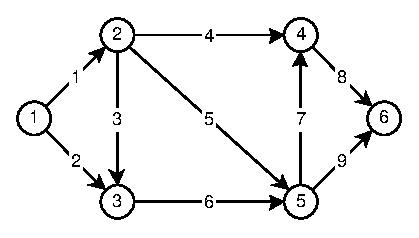
\includegraphics[width=\textwidth]{Chapter_I/1/1_1a.eps}
		\caption{}
	\end{subfigure}%
	%add desired spacing between images, e. g. ~, \quad, \qquad, \hfill etc.
	%(or a blank line to force the subfigure onto a new line)
	\qquad
	\begin{subfigure}[b]{0.45\textwidth}
		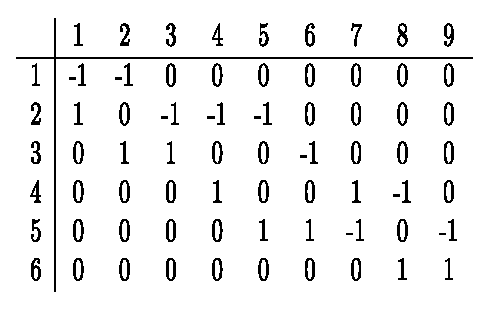
\includegraphics[width=\textwidth]{Chapter_I/1/1_1b.eps}
		\caption{}
	\end{subfigure}
	\caption{\textbf{Macierz incydencji} \textbf{(a)} Graf skierowany $G = \left( V, E \right)$ z identyfikatorami węzłów $1-6$ i łuków $1-9$ (dla znanych identyfikatorów łuków będziemy stosować oznaczenie $e_{i}$ zamiast $e_{pk}$). \textbf{(b)} Macierz incydencji $ \left| V \right| \times \left| E \right| $ grafu $G$.}\label{fig:incidenceMatrix}
\end{figure}

Operacje, jakie będziemy chcieli - jak się później okaże - wykonywać na tak zdefiniowanej macierzy (i na każdej następnej strukturze z tego podrozdziału) to procedury wyszukiwania wszystkich bezpośrednich następników danego węzła $v_{i}$ (oznaczać będziemy taki zbiór za pomocą symbolu $A \left( i \right) $) i odnajdywania każdego takiego łuku, wychodzącego z danego węzła do wszystkich $v_{k} \in A \left( i \right) $. Dla pierwszego podejścia:

\begin{myitemize}
	\item koszt identyfikacji wszystkich łuków jest ściśle powiązany z ilością krawędzi w grafie - wystarczy, że dla wierzchołka $v_{i}$ przejrzymy cały jeden wiersz o indeksie $i$, aby odnaleźć identyfikatory wszystkich krawędzi, bezpośrednio wychodzących z danego wierzchołka (wszystkie komórki o wartości mniejszej od zera). Możemy ograniczyć ilość potrzebnych skanowań poprzez wprowadzenie licznika krawędzi wychodzących, lecz w najgorszym możliwym przypadku takie skanowanie wciąż będzie wymagało $O \left( m \right)$ porównań, gdzie $m$ to oczywiście liczba krawędzi w grafie.
	\item Koszt wyszukiwania wszystkich następników węzła $v_{i}$, obejmuje koszt wyszukania wszystkich łuków, prowadzących do tych wierzchołków oraz odnalezienie ich identyfikatorów - co dla każdego odnalezionego łuku $e_{j}$ zmusza nas do przeszukania wszystkich elementów macierzy, znajdujących się w tej samej, $j$'tej kolumnie. Takich kolumn, jak wspomnieliśmy wcześniej, będzie $ \left| A \left( i \right) \right| $, przeszukanie każdej $j$'tej kolumny wymagać będzie, w najgorszym przypadku, $n-1$ porównań dla każdej z nich tak więc ostatecznie otrzymujemy $O \left( \left| A \left( i \right) \right| \cdot n \right)$ dla wyszukiwania wszystkich następników węzła $v_{i}$ (wraz z wyszukiwaniem łuków $O \left( m + \left| A \left( i \right) \right| \cdot n \right)$).
\end{myitemize}

\subsection{Macierz sąsiedztwa}

Oprócz macierzowej reprezentacji typu wierzchołek-krawędź możliwe jest także reprezentowanie struktury grafu za pomocą macierzy typu wierzchołek-wierzchołek. \textbf{Macierz sąsiedztwa} dla grafu $G = \left( V, E \right) $ jest to macierz o wymiarach $\left| V \right| \times \left| V \right|$, gdzie wartość każdej komórki jest zdefiniowana następująco:

\begin{equation}
	b_{ij}= \left\{ 
	\begin{array}{ll}
	1 & \textrm{jeżeli istnieje ścieżka z wierzchołka $v_{i}$ do $v_{j}$,}\\
	0 & \textrm{w przeciwnym wypadku}
	\end{array} \right.
\end{equation}


O ile, w przypadku takiego przedstawienia grafu, jesteśmy w stanie uzyskać informacje o wszystkich bezpośrednich następnikach dowolnego węzła w czasie liniowym (dla węzła $v_{i}$ wystarczy przeszukać wiersz o indeksie $i$) to macierz w takiej postaci nie niesie ze sobą istotnych informacji o krawędziach grafu - takich, które umożliwiłyby ich szybką identyfikację, nie zmuszając nas do ponownego przeglądania wszystkich krawędzi grafu w poszukiwaniu łuku, który ma swój początek i koniec w - danych nam przez macierz - wierzchołkach. Umiejętność szybkiej identyfikacji takich krawędzi będzie nam w późniejszych rozważaniach nieodzowna, jako że chcemy się skupić na wyszukiwaniu najkrótszych ścieżek, gdzie kluczowych informacji dla tego problemu będziemy szukać właśnie w krawędziach między wierzchołkami. Załóżmy, że każda krawędź będzie określana za pomocą trzech cech: wierzchołka startowego, końcowego oraz odległości między tymi dwoma punktami. Zauważmy, że w takim przypadku wszystkie informacje o krawędzi możemy umieścić bezpośrednio w macierzy sąsiedztwa, zastępując starą definicję nową: 

\begin{equation}
	b_{ij}= \left\{ 
	\begin{array}{ll}
	$ d ( i, j ) $ & \textrm{jeżeli istnieje ścieżka z wierzchołka $v_{i}$ do $v_{j}$,}\\
	0 & \textrm{w przeciwnym wypadku}
	\end{array} \right.
\end{equation}

gdzie przez $ d \left( i,j \right) $ zwykle będziemy oznaczać długość ścieżki (odległość między wierzchołkami, które łączy). Takie podejście pozwala nam na nie tworzyć dodatkowych struktur, przechowujących informacje o krawędziach. Jeżeli chcielibyśmy wzbogacać naszą strukturę krawędzi wygodniej (a także bezpieczniej) zamiast wartości $d \left( i,j \right)$ w danych komórkach $b_{ij}$ będzie wstawić numer identyfikatora danej krawędzi. Zapewni nam to dodatkowo jednoznaczność w przypadku chęci identyfikacji krawędzi (zwróćmy uwagę, że oba łuki, wchodzące do węzła $v_{4}$ mają ten sam koszt $ d \left( 2, 4 \right) = d \left( 5, 4 \right) = 2$, co uniemożliwia nam ich rozróżnienie).

\begin{figure}[!htbp]
	\centering
	\begin{subfigure}[b]{0.45\textwidth}
		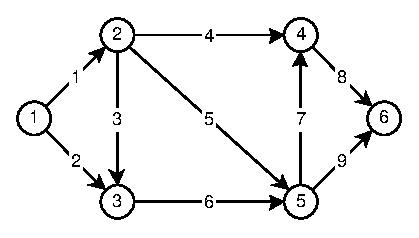
\includegraphics[width=\textwidth]{Chapter_I/2/1_2a.eps}
		\caption{}
	\end{subfigure}
	\qquad
	\begin{subfigure}[b]{0.09\textwidth}
		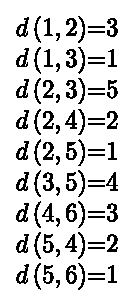
\includegraphics[width=\textwidth]{Chapter_I/2/1_2b.eps}
		\caption{}
	\end{subfigure}
	\qquad
	\begin{subfigure}[b]{0.35\textwidth}
		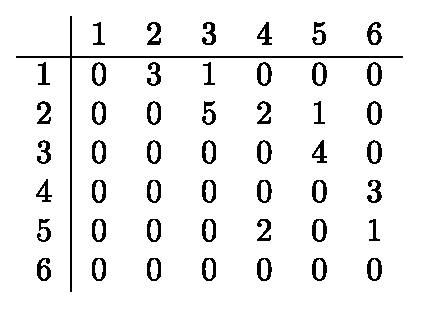
\includegraphics[width=\textwidth]{Chapter_I/2/1_2c.eps}
		\caption{}
	\end{subfigure}
	\caption{\textbf{Macierz sąsiedztwa} \textbf{(a)} Graf skierowany $G = \left( V, E \right)$ z identyfikatorami węzłów $1-6$ i łuków $1-9$. \textbf{(b)} Wagi/koszty łuków grafu $G$. \textbf{(c)} Macierz sąsiedztwa $ \left| V \right| \times \left| V \right| $ grafu $G$. Dla każdej wagi łuku $ d \left( v_{p}^{ID}, v_{k}^{ID} \right) = c$ odpowiednie komórki na przecięciu wiersza o numerze $v_{p}^{ID}$ i kolumny $v_{k}^{ID}$ mają wartość równą $c$, gdzie $v_{k}^{ID}$ oznacza identyfikator węzła $v_{k}$ ( $v_{k}^{ID} = k$).}\label{fig:adjacencyMatrix}
\end{figure}

Zatem ostatecznie otrzymamy:

\begin{myitemize}
	\item koszt identyfikacji wszystkich łuków o złożoności liniowej $O \left( n \right)$, gdzie $ n = \left| V \right| $,
	\item koszt wyszukiwania wszystkich następników węzła $v_{i}$ w tym przypadku jest tożsamy z odnalezieniem wszystkich łuków wychodzących z danego węzła, co zajmuje $O \left( n \right)$.
\end{myitemize}

\subsection{Listy incydencji}

Wprowadzone wcześniej przez nas oznaczenie $A \left( i \right) $, oznaczające wszystkich bezpośrednich następników danego węzła $v_{i}$ od teraz będzie dla nas oznaczało jednokierunkową listę łuków, wychodzących z węzła $v_{i}$ oraz wchodzących do każdego węzła $v_{k} \in A \left( i \right)$ (ang. \textit{Adjacency list}), a operacja wyszukania takich łuków będzie dla nas tożsama ze znalezieniem wszystkich wierzchołków $v_{k}$. Słowem - połączymy poprzednio rozdzielane operacje identyfikacji łuków i węzłów w jedną. Da to nam w najgorszym przypadku liniowy czas dostępu do dowolnego wierzchołka, będącego bezpośrednim następnikiem badanego elementu (gdy będziemy musieli przejść przez całą listę $A \left( i \right) $). 

\begin{figure}[!htbp]
	\centering
	\begin{subfigure}[b]{0.57\textwidth}
		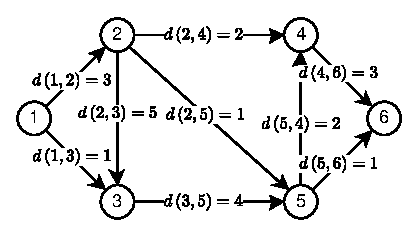
\includegraphics[width=\textwidth]{Chapter_I/3/1_3a.eps}
		\caption{}
	\end{subfigure}%
	%add desired spacing between images, e. g. ~, \quad, \qquad, \hfill etc.
	%(or a blank line to force the subfigure onto a new line)
	\qquad
	\begin{subfigure}[b]{0.33\textwidth}
		
\includegraphics[width=\textwidth]{Chapter_I/3/1_3b.eps}
		\caption{}
	\end{subfigure}
	\caption{\textbf{Lista sąsiedztwa} \textbf{(a)} Graf skierowany $G = \left( V, E \right)$ z identyfikatorami węzłów $1-6$. Zamiast identyfikatorów łuków na krawędziach zostały naniesione wagi każdego z nich. \textbf{(b)} Listy sąsiedztw grafu $G$. Dla każdego węzła $v_{i} : i \in \left\{ 1, \ldots, 6 \right\}$ jest stworzona lista jednokierunkowa, której każdy element zawiera informację o pojedynczym łuku $e_{ij}$.}\label{fig:adjacencyList}
\end{figure}

Każdy taki łuk, oprócz swojej długości (dalej zwanej ogólniej: \textbf{kosztem}) będzie zatem posiadał dodatkowy atrybut, jednoznacznie wskazujący na węzeł, do którego prowadzi. Formalnie:

$v_{k} \in A \left ( i \right ) \Leftrightarrow \exists e_{ik} = \left( v_{i}, v_{k} \right) \in E $

Taką strukturę będziemy dalej nazywać zamiennie listą sąsiedztwa lub \textbf{incydencji} \footnote{Mówimy, że dwa wierzchołki są incydentne, jeżeli istnieje łącząca je krawędź.}.

\subsection{Pęki}

Na podobnym pomyśle, co listy sąsiedztwa, bazuje rozwiązanie z użyciem tzw. pęków. Tutaj także dla każdego węzła tworzyć będziemy ,,listę'' węzłów, które są jego bezpośrednimi następnikami z tą różnicą, że te informacje będziemy zapisywać w jednej tablicy, nie na osobnych listach.

W niniejszym podrozdziale omówimy najbogatszą wersję reprezentacji z jednoczesnym wykorzystaniem \textbf{pęków wyjściowych} jak i \textbf{ wejściowych} (ang. \textit{Forward and Reverse Star Representation}), koncentrując się po kolei na pierwsze i drugiej części, które równie dobrze mogą stanowić samodzielne reprezentacje grafów.

\subsubsection{Pęki wyjściowe}

Załóżmy, że nasza reprezentacja grafu zawiera tablicę indeksowaną od $1$ do $ \left| V \right| $ - nazwijmy ją $vtab$. Stwórzmy drugą tablicę, która będzie konstruowana następująco:

dla każdego elementu tablicy $vtab$ o indeksie $vIdx$ (indeksy tej tablicy odpowiadają identyfikatorom wszystkich węzłów w grafie) będziemy chcieli, aby wartość, przechowywana w tej komórce, była równa minimalnemu indeksowi $aIdx$ w tablicy $atab$, dla którego element $atab \left[ aIdx \right] $ będzie zawierał informacje o łuku, wychodzącym z wierzchołka o identyfikatorze $vIdx$, zaś wartość $vtab \left[ vIdx+1 \right] $ będzie zawierała ostatni taki indeks, powiększony o jeden. Innymi słowy będziemy chcieli aby każdy element z tablicy $vtab$ zawierał informację o tym, od którego miejsca w tablicy $atab$ są przechowywane kolejno wszystkie informacje o łukach, wychodzących z węzła, przechowywanego w badanym elemencie pierwszej tablicy (rys. \ref{fig:forwardStarRepresentation}).

\begin{figure}[!htbp]
	\centering
	\begin{subfigure}[b]{0.5\textwidth}
		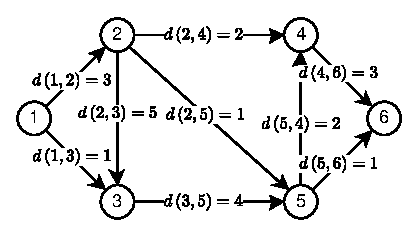
\includegraphics[width=\textwidth]{Chapter_I/4/1_4a.eps}
		\caption{}
	\end{subfigure}%
	\qquad
	\begin{subfigure}[b]{0.4\textwidth}
		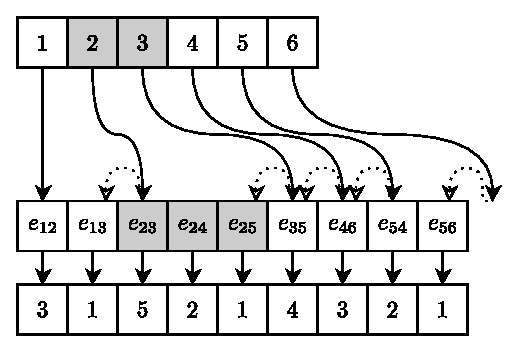
\includegraphics[width=\textwidth]{Chapter_I/4/1_4b.eps}
		\caption{}
	\end{subfigure}
	\caption{\textbf{Pęki wyjściowe} \textbf{(a)} Graf skierowany $G = \left( V, E \right)$ z identyfikatorami węzłów $1-6$. \textbf{(b)} Pęki łuków dla grafu $G$. Dla każdego węzła $v_{i} \in vtab$ element $ vtab \left[ i \right] $ zawiera indeks pierwszej, wychodzącej krawędzi z węzła $v_{i}$ w tablicy $atab$. Elementy w $atab$ są z kolei wskazaniami na odpowiednie krawędzie grafu.}\label{fig:forwardStarRepresentation}
\end{figure}

Na początku musimy stworzyć obie tablice, pierwszą ($vtab$) zainicjować samymi jedynkami (numer pierwszego indeksu łuku), zaś drugą pozostawić pustą - będziemy ją wypełniać w trakcie działania algorytmu. Następnie, iterując po tablicy z wierzchołkami $vtab$ odnajdujemy wszystkie łuki wychodzące z danego wierzchołka i wstawiamy dane takiej krawędzi (zakładamy, że są nimi identyfikatory łuków) do kolejnych elementów tablicy $atab$, jednocześnie zwiększając licznik $aIdx$. Gdy przeglądniemy wszystkie łuki wychodzące z pierwszego wierzchołka $v_{vIdx}$, wstawiamy do następnego elementu z tablicy $vtab$ ($vtab \left[ vIdx+1 \right] $) wartość licznika $aIdx$ - jest to najmniejszy indeks w tablicy $atab$, dla którego element $atab \left[ aIdx \right] $ będzie zawierał identyfikator łuku, wychodzącego z wierzchołka $v_{vIdx+1}$, a tym samym łatwo będziemy mogli policzyć, który element w tablicy zawiera ostatni łuk, wychodzący z wierzchołka poprzedniego (o indeksie $vIdx$). Algorytm kontynuujemy, dopóki nie przeglądniemy wszystkich elementów w tablicy $vtab$. W efekcie otrzymamy tablicę $atab$, której elementy będą posortowane rosnąco względem identyfikatorów wierzchołków, z których wychodzą, a każda para elementów $ \left( vtab \left[ i \right] , vtab \left[ i+1 \right] \right) $ będzie zawierać indeksy, dla których od $atab \left[ vtab \left[ i \right] \right] $ do $atab \left[ vtab \left[ i+1 \right] -1 \right] $ znajdują się łuki wychodzące z wierzchołka o indeksie $i$.

Jeżeli okaże się, że jakiś wierzchołek $v_{i}$ nie ma żadnych krawędzi wychodzących, wtedy $vtab \left[ i \right] = vtab \left[ i+1 \right] $, w szczególności $vtab \left[ 1 \right] = 1$ (pierwszy element, jako że indeksujemy od jedynki).

\begin{algorithm}[!htbp]
\DontPrintSemicolon
\KwData{$G= \left( V, E \right) $}
\KwResult{$atab \left[ 1 \ldots \left| E \right| \right] $}
\Begin{
	$aIdx \longleftarrow 1$\;
	$vtab \left[ 1 \ldots \left| V \right| \right] \longleftarrow aIdx$\;
	\For(\tcc*[f]{Dla każdego węzła w $vtab$}){$vIdx\in 1 \ldots \left| V \right| $}{
		\For{każdy łuk $e$, prowadząca z $v_{vIdx}$ do wierzchołka $\in A \left( vIdx \right) $}{
			$atab[aIdx] = e$\;
			$aIdx \longleftarrow aIdx + 1$\;
		}
	$vtab \left[ vIdx+1 \right] \longleftarrow aIdx$\; 
	}
}
\caption{CREATE-FORWARD-STAR-REPRESENTATION\label{alg:cfsr}}
\end{algorithm}


\subsubsection{Pęki wejściowe}

Mamy sytuację odwrotną: chcemy mieć możliwość szybkiego zidentyfikowania wszystkich wierzchołków wchodzących do danego węzła $v_{k}$. Algorytm jest taki sam jak w poprzednim przypadku z tą różnicą, że kolejność występowania łuków w tablicy $atab$ będzie inna - będą one występować w kolejności rosnących identyfikatorów węzłów, do których prowadzą, a nie mają początek. W obu przypadkach kolejność występowania krawędzi, wychodzących/prowadzących do tych samych wierzchołków nie ma znaczenia - w algorytmach wyszukiwania najkrótszych ścieżek, jeżeli zapytamy o dany węzeł to będziemy chcieli poznać wszystkich jego bezpośrednich następników/poprzedników, a nie tylko wybranego z nich.

\subsubsection{Pęki wejścia-wyjścia}

W pewnych przypadkach warto abyśmy dysponowali możliwością nie tylko szybkiego przeglądania tablic incydencji w poszukiwaniu następników, ale chcielibyśmy także mieć taką możliwość w odniesieniu do wszystkich poprzedników dowolnego węzła w sieci. Aby zrobić to oszczędnie, będziemy wykorzystywać fakt, że we wcześniejszych wersjach w tablicy $atab$ celowo trzymaliśmy tylko identyfikatory łuków, nie zaś ich wszystkie atrybuty (np. dla łuku o identyfikatorze $i$ o atrybutach: węzeł początkowy, końcowy oraz koszt, wartości te trzymalibyśmy w elementach osobnych tablic: $head \left[ i \right] $,  $tail \left[ i \right] $ oraz  $cost \left[ i \right] $). Jako podstawę dla naszego algorytmu weźmiemy pierwszą z omawianych reprezentacji, a więc zakładamy, że mamy tablice:

\begin{myitemize}
	\item $ vtab \left[ 1 \ldots \left| V \right| \right] $ - przechowującą informacje o łukach dla węzłów o identyfikatorach od $1$ do $ \left| V \right| $,
	\item $atab \left[ 1 \ldots \left| E \right| \right] $ - przechowującą krawędzie o identyfikatorach od $1$ do $ \left| E \right| $, posortowane rosnąco według identyfikatorów wierzchołków początkowych, gdzie dla każdego węzła $v_{k}$ wszystkie identyfikatory łuków wychodzących z tego węzła znajdują się w elementach od $atab \left[ vtab \left[ k \right] \right] $ do $atab \left[ vtab \left[ k+1 \right] -1 \right] $ włącznie
\end{myitemize}

i do nich chcemy dodać dwie nowe:

\begin{myitemize}
	\item $rtab \left[ 1 \ldots \left| V \right| \right] $ - analogicznie do $vtab$ przechowującą informacje o łukach dla węzłów o identyfikatorach od $1$ do $ \left| V \right| $ (dla reprezentacji odwróconej - \textit{Reverse Star Representation}),
	\item $mtab \left[ 1 \ldots \left| E \right| \right] $ - mapującą krawędzie o identyfikatorach od $1$ do $ \left| E \right| $.
\end{myitemize}

Druga z nich - $mtab$ - jest tablicą wejściową dla metody, opisanej w sekcji ,,Pęki wejściowe''. Przechowuje ona w swoich kolejnych elementach indeksy tablicy $atab$ w taki sposób, aby ciąg \\ $atab \left[ mtab \left[ 1 \right] \right], atab \left[ mtab \left[ 2 \right] \right], \ldots, atab \left[ mtab \left[ \left| E \right| \right] \right] $ tworzył ciąg identyfikatorów łuków, które są posortowane rosnąco wedle wierzchołków wejściowych. Wówczas tablica $rtab$ razem z tablicą $mtab$ zachowuje się dokładnie tak samo jak druga para tablic.

\begin{figure}[!htbp]
	\centering
	\begin{subfigure}[b]{0.32\textwidth}
		\begin{subfigure}[b]{1\textwidth}
			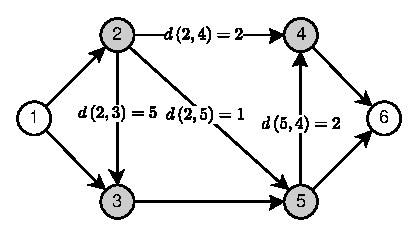
\includegraphics[width=\textwidth]{Chapter_I/5/1_5a.eps}
			\caption{}
		\end{subfigure}
		\begin{subfigure}[b]{1\textwidth}
			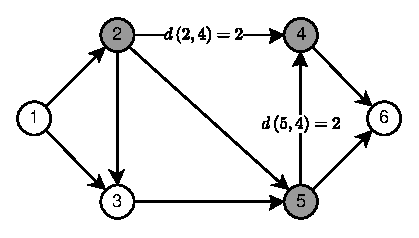
\includegraphics[width=\textwidth]{Chapter_I/5/1_5b.eps}
			\caption{}
		\end{subfigure}
	\end{subfigure}
	\qquad
	\begin{subfigure}[b]{0.50\textwidth}
		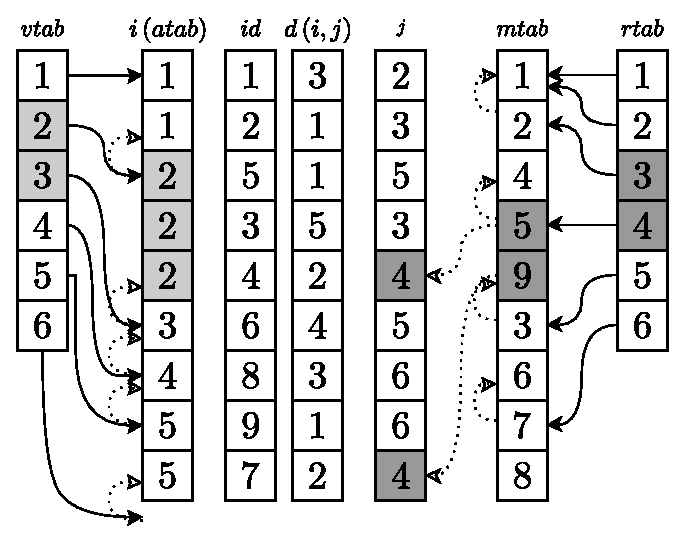
\includegraphics[width=\textwidth]{Chapter_I/5/1_5c.eps}
		\caption{}
	\end{subfigure}
	\caption{\textbf{Pęki wejścia-wyjścia} \textbf{(a)} Reprezentacja grafu $G = \left( V, E \right)$ z oznaczonymi następnikami węzła $v_{2}$. \textbf{(b)} Ten sam graf skierowany z oznaczonymi poprzednikami węzła $v_{2}$. \textbf{(c)} Graf przedstawiony w formie tablic.}\label{fig:forwardReverseStarRepresentation}
\end{figure}

Oczywiście taki sposób reprezentacji danych jest bardzo wrażliwy na wszelkie zmiany w strukturze sieci - każde usunięcie czy dodanie krawędzi powoduje konieczność aktualizacji wszystkich tablic, co jest bardzo pracochłonne, w porównaniu z reprezentacjami macierzowymi (gdzie taka operacja mogła być wykonana w czasie stałym) czy przy wykorzystaniu list sąsiedztwa (gdzie koszt dodawania krawędzi jest także stały, zaś koszt jej usunięcia to czas rzędu $ O \left( \left| E \right| \right) $). Taka reprezentacja natomiast pozwala nam na błyskawiczne - bo polegające na odjęciu wartości $vtab \left[ i \right] $ od $vtab \left[ i+1 \right] $ - policzenie \textbf{stopnia} wierzchołka $v_{i}$, a także uzyskać dostęp do wszystkich elementów $ v \in A \left( i \right) $ dla dowolnego wierzchołka $v_{i}$ w tym samym, liniowym, zależnym od ilości elementów w $A \left( i \right) $, czasie, jednocześnie przy zachowaniu stosunkowo małego - bo także liniowego - zapotrzebowania na pamięć (rys. \ref{fig:forwardReverseStarRepresentation}).

\subsection{Złożoność pamięciowa i czasowa}

Innym kryterium wyboru najodpowiedniejszego sposobu przedstawienia grafu jest ilość pamięci, jakiej wymagają implementacje poszczególnych rozwiązań. Dla obu implementacji macierzowych będą to wymagania rzędu $O \left( \left| V \right| \ldots \left| E \right| \right)$ lub $O \left( \left| V \right| \ldots \left| V \right| \right)$, odpowiednio dla macierzy incydencji i sąsiedztwa. Ile tak naprawdę z tej pamięci jest przez nas marnowanej najlepiej widać w przypadku, gdy mamy do czynienia z \textbf{grafem rzadkim} \footnote{graf, którego stosunek posiadanych krawędzi do ilości węzłów w danym grafie jest niewielki}, gdzie w takiej sytuacji większość macierzy jest wypełniona zerami (macierz rzadka). Stosując odpowiednie kodowanie, możemy wpłynąć na tą niepożądaną własność np. macierz incydencji, której elementy $a_{ij}$ posiadają tylko trzy wartości: $-1, 0, 1$ możemy przedstawić za pomocą dwóch macierzy, z której jedna - nazwijmy ją macierzą wyjścia - będzie zawierać jedynki na tych samych pozycjach, co poprzednia macierz, lecz w miejscach wystąpienia wartości ujemnej będzie miała wartość równą zero. Dla macierzy wejścia z kolei będziemy wstawiać jedynki w miejscach, gdzie uprzednio znajdowały się wartości przeciwne.

\begin{equation}
	a^{IN}_{ij}= \left\{ 
	\begin{array}{ll}
	1 & \textrm{jeżeli $a_{ij} = -1$,}\\
	0 & \textrm{w przeciwnym wypadku}
	\end{array} \right.
\end{equation}

\begin{equation}
	a^{OUT}_{ij}= \left\{ 
	\begin{array}{ll}
	1 & \textrm{jeżeli $a_{ij} = 1$,}\\
	0 & \textrm{w przeciwnym wypadku}
	\end{array} \right.
\end{equation}

Następnie zamieniamy każdą macierz na ciągi binarne długości $ \left| V \right| \ldots \left| E \right| $ każdy. Jest to prosta metoda na zgromadzenie potrzebnych nam informacji na jak najmniejszym fragmencie pamięci (jedna informacja - 1 bit), dodatkowo umożliwiająca nam bardzo szybkie przeszukiwanie takiej macierzy za pomocą operacji bitowych, a wykonanie kopii tak zgromadzonych danych to już nie koszt skopiowania wartości każdego elementu macierzy, a przepisanie jednej, potencjalnie olbrzymiej, liczby. Jednakże taka metoda wpływa tylko na obniżenie stałej i asymptotycznie nie daje żadnych widocznych różnic, jeżeli mówimy o złożoności pamięciowej, gdyż nadal pamiętamy $\left| V \right| \cdot \left| E \right|$ elementów.

W przypadku macierzy sąsiedztwa złożoność pamięciowa wynosi $O \left( \left| V \right| ^{2} \right) $, co nie powinno być dla nas zaskoczeniem, gdyż na obu osiach macierzy znajdują się wszystkie wierzchołki grafu. Oczywistym także jest, że zapotrzebowanie na pamięć będzie wzrastać im więcej informacji będziemy chcieć przechowywać w komórkach macierzy.

Dla samych list sąsiedztwa będziemy potrzebowali $O \left( \left| E \right| \right) $ pamięci, gdzie stała znowu może się różnić, w zależności od tego ile danych będziemy chcieli przechowywać w elementach list. Podczas tworzenia $ \left| V \right| $ list incydencji mamy zagwarantowane, że żadnego łuku nie dodamy dwa razy oraz, że wszystkie łuki w grafie zostaną do nich dodane (łuk z definicji ma tylko jeden początek i koniec, więc jeśli dany łuk $e \in A \left( i \right)$ dla węzła $v_{i}$ to na pewno nie należy do żadnego $A \left( j \right)$, gdzie $j \neq i$). Stąd elementów na wszystkich $ \left| V \right| $ listach sąsiedztwa jest dokładnie $ \left| E \right| $ elementów. Łącznie zatem, aby zaimplementować rozwiązania oparte na listach sąsiedztwa, potrzebujemy $ O \left( \left| V \right| + \left| E \right| \right)$ pamięci.

Mamy zatem:

~

\begin{savenotes}
	\begin{center}
		\begin{tabular}{ccccc}
			\hline
			& \multicolumn{2}{c}{Macierze} & \multicolumn{1}{c}{Listy} & \multicolumn{1}{c}{Pęki} \\
			& Incydencji & Sąsiedztwa & Sąsiedztwa & Wejścia-wyjścia \\
			\hline
			Potrzebna pamięć & $ O \left( \left| V \right| \cdot \left| E \right| \right) $  & $ O \left( \left| V \right| ^{2} \right)$ & $ O \left( \left| V \right| + \left| E \right| \right)$ & $ O \left( \left| V \right| + \left| E \right| \right)$ \\
			\hline
			Przegląd $v \in A \left( i \right) $ & $O \left( \left| E \right| + \left| A \left( i \right) \right| \cdot \left| V \right| \right)$ & $O \left( \left| V \right| \right) $ & $O \left( \left| A \left( i \right) \right| \right) $ & $O \left( \left| A \left( i \right) \right| \right) $ \\
			\hline
			Dodawanie krawędzi \footnote{W przypadku dodawania krawędzi znamy identyfikatory obu węzłów, z którymi połączony ma być dodawany łuk.} & $O \left( 1 \right)$ & $O \left( 1 \right) $ & $O \left( 1 \right) $ & $O \left( \left| V \right| + \left| E \right| \right) $ \\
			Dodawanie nowej krawędzi & $ O \left( \left| V \right| \cdot \left| E \right| \right) $ & $ O \left( 1 \right) $ & $O \left( 1 \right) $ & $O \left( \left| V \right| + \left| E \right| \right) $ \\
			Usuwanie krawędzi \footnote{Poza ostatnim przypadkiem, znany jest tylko identyfikator łuku i węzła, do którego dana krawędź prowadzi. Nie dotyczy to reprezentacji opartej na pękach wejścia-wyjścia, gdzie znajomość identyfikatora, jaki posiada łuk, daje nam dostęp do identyfikatorów obu węzłów, które ta krawędź łączy.} & $O \left( \left| V \right| \right)$ & $O \left( \left| V \right| \right) $ & $O \left( \left| E \right| \right) $ & $O \left( \left| V \right| + \left| E \right| \right)$ \\
			Trwałe usuwanie krawędzi & $ O \left( \left| V \right| \cdot \left| E \right| \right) $ & $ O \left( \left| V \right| \cdot \left| E \right| \right) $ & $O \left( \left| E \right| \right) $ & $O \left( \left| V \right| + \left| E \right| \right)$ \\
			Stopień wierzchołka & $O \left( \left| E \right| \right)$ & $O \left( \left| V \right| \right) $ & $O \left( \left| A \left( i \right) \right| \right) $ & $O \left( 1 \right) $ \\
		\end{tabular}
	\end{center}
\end{savenotes}

~

Jak widać rozdzieliliśmy operacje dodawania i usuwania elementów grafu, wyróżniając takie, które mają na celu tylko ,,zakryć'' obecność danego elementu, bądź z powrotem przywrócić jego widoczność oraz na takie, których celem jest permanentna modyfikacja, przechowywanego w pamięci, grafu. Różnicę między tymi operacjami bardzo wyraźnie widać w przypadku korzystania z reprezentacji macierzowych grafu, gdzie ,,usunięcie'' krawędzi możemy przeprowadzić w czasie zdecydowanie krótszym, niż byśmy mieli zmieniać rozmiar samych macierzy poprzez usuwanie/dodawanie elementów na którejkolwiek z ich osi. Chcąc ,,usunąć'' z grafu daną krawędź wystarczy abyśmy zlokalizowali węzły, z którymi ma ona połączenie i w odpowiednich komórkach macierzy zamazali zapis o istniejącym połączeniu (założyliśmy, że w nasze grafy są skierowane tak więc znając łuk, który chcemy usunąć, mamy informację tylko o węźle, do którego dany łuk prowadzi - w obu przypadkach reprezentacji macierzowych zmusza nas to do dodatkowego przeszukania jednej z wybranych kolumn, w celu odszukania węzła, z którego łuk, który chcemy usunąć, wychodzi). Krawędź w grafie nadal będzie istnieć, lecz stanie się ona bezużyteczna, a dla algorytmów niezauważalna. Należy jednak tutaj podkreślić, że za takie traktowanie danych przyjdzie nam zapłacić, utrzymującym się na stałym poziomie, kosztem przeglądania macierzy w poszukiwaniu następników interesujących nas węzłów, zaś poza macierzowymi reprezentacjami różnice pomiędzy trwałym, a tymczasowym usuwaniem elementów nie ma żadnego wpływu na złożoność obliczeniową bez dodatkowych modyfikacji przedstawionych struktur.

~
\begin{center}
	\begin{tabular}{ccccc}
		\hline
		& \multicolumn{2}{c}{Macierze} & \multicolumn{1}{c}{Listy} & \multicolumn{1}{c}{Pęki} \\
		& Incydencji & Sąsiedztwa & Sąsiedztwa & Wejścia-wyjścia \\
		\hline
		Dodawanie węzła & $ O \left( \left| V \right| \cdot \left| E \right| \right) $ & $ O \left( 1 \right) $ & $O \left( 1 \right) $ & $O \left( \left| V \right| + \left| E \right| \right) $ \\
		Dodanie nowego  węzła & $ O \left( \left| V \right| \cdot \left| E \right| \right) $  & $ O \left( \left| V \right| ^{2} \right)$ & $ O \left( 1 \right)$ & $ O \left( \left| V \right| \right)$ \\
		Przysłonięcie węzła & $ O \left( \left| V \right| \cdot \left| E \right| \right) $  & $ O \left( \left| V \right| \right)$ & $ O \left( \left| E \right| \right)$ & $ O \left( \left| V \right| + \left| E \right| \right)$ \\
		Trwałe usunięcie węzła & $ O \left( \left| V \right| \cdot \left| E \right| \right) $  & $ O \left( \left| V \right| ^{2} \right)$ & $ O \left( \left| E \right| \right)$ & $ O \left( \left| V \right| + \left| E \right| \right)$ \\
	\end{tabular}
\end{center}

~

Poza takimi operacjami jak: dodawanie, usuwanie krawędzi grafu, wyznaczanie stopnia wierzchołka, jego następników możemy także chcieć na bieżąco modyfikować ilość węzłów, jakie znajdują się w grafie. Poniżej przedstawiono zestawienie czasów trwania wymienionych operacji dla wszystkich omówionych sposobów reprezentacji grafu. Podobnie jak w poprzednim przypadku, dla macierzy incydencji potrafimy wykonać operację ,,usuwania'' węzła bez faktycznej zmiany rozmiarów tych macierzy, jednak w tym wypadku zysk z takiego postępowania jest niewielki, by wręcz nie powiedzieć: asymptotycznie żaden - podstawowym pomysłem na wymazanie informacji o danym węźle jest usunięcie wszystkich danych o łukach, które do niego prowadzą tak, aby węzeł przestał być osiągalny, lecz (jak pokazaliśmy wyżej) każdorazowa operacja samego wymazania informacji o pojedynczej krawędzi już kosztuje nas $O \left( \left| V \right| \right) $. W najgorszym przypadku musielibyśmy usunąć wszystkie krawędzie w grafie, co daje nam łącznie złożoność operacji tymczasowego usuwania węzła $O \left( \left| V \right| \cdot  \left| E \right| \right) $. 

Nieco lepsze rezultaty jesteśmy w stanie osiągnąć z macierzami sąsiedztw, gdyż w tym przypadku odnalezienie wiersza/kolumny z danym węzłem, który chcemy usunąć, jest równoznaczne z odnalezieniem wszystkich łuków, które do niego prowadzą i, gdybyśmy zignorowali konieczność zmiany rozmiaru całej macierzy (chcieli tylko ukryć jej elementy), to otrzymalibyśmy górne ograniczenie na złożoność tej operacji na poziomie $ O \left( \left| V \right| \right)$.

\begin{figure}[!htbp]
	\centering
	\begin{subfigure}[b]{0.5\textwidth}
		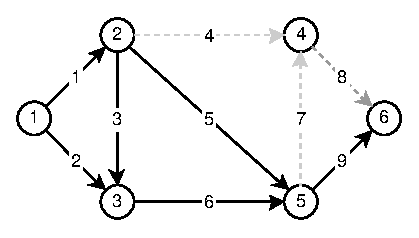
\includegraphics[width=\textwidth]{Chapter_I/6/1_6a.eps}
		\caption{}
	\end{subfigure}%
	\qquad
	\begin{subfigure}[b]{0.4\textwidth}
		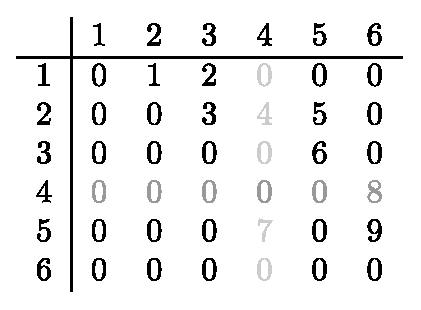
\includegraphics[width=\textwidth]{Chapter_I/6/1_6b.eps}
		\caption{}
	\end{subfigure}
	\caption{\textbf{Ukrycie węzła w macierzy sąsiedztwa} \textbf{(a)} Graf skierowany $G = \left( V, E \right)$. \textbf{(b)} Macierz sąsiedztwa dla grafu $G$. Chcemy ukryć w niej informację o $v_{4}$ tak, aby nie był on osiągalny z żadnego innego węzła w grafie. }\label{fig:adjacencyMatrixHideNode}
\end{figure}

Dla takiej koncepcji, dodanie na powrót węzła do grafu jest tylko kwestią dodania jakiegokolwiek łuku, który będzie łączył istniejący w sieci węzeł z tym, który chcemy dodać, więc koszty tej operacji będą identyczne, do dla dodawania krawędzi z poprzedniej tabeli.

W przypadku pozostałych dwóch struktur znowu nie odnotujemy żadnej zmiany - aby usunąć dany węzeł z list sąsiedztwa będziemy musieli odnaleźć wszystkie łuki, które prowadzą do usuwanego węzła, a na koniec usunąć całą listę jego sąsiedztwa, wraz z łukami, które się na niej znajdują. W najgorszym przypadku będzie od nas to wymagało przeglądnięcia wszystkich krawędzi, występujących w grafie, co uczynimy w czasie $ O \left( \left| E \right| \right) $. Dla pęków operacja usunięcia węzła jest jeszcze bardziej skomplikowana, gdyż nie istnieje w niej możliwość zaznaczenia konkretnego węzła, który chcielibyśmy ukryć, zaś jego usunięcie wymaga od nas odnalezienia obu zbiorów krawędzi (wychodzących z usuwanego węzła oraz do niego wchodzących), usunięcie ich z tablic, przechowujących o nich informacje (co uczynimy w czasie $ O \left( A \left( i \right) + A^{R} \left( i \right) \right) $ \footnote{Poprzez $A^{R} \left( i \right) $ oznaczać będziemy zbiór sąsiadów węzła $v_{i}$, lecz będą to węzły bezpośrednio ten węzeł poprzedzające, z których krawędzie prowadzą do tego węzła.}, zmiany ich rozmiarów ($ O \left( \left| E \right| \right) $), usunięcia danego węzła z dwóch pozostałych tablic, indeksowanych od $ 1 \ldots \left| V \right| $ (oraz zmiana ich rozmiarów - $ O \left( \left| V \right| \right) $)) oraz na końcu aktualizacji tych ostatnich ($ O \left( \left| V \right| \right) $) wraz z pomocniczą tablicą $mtab$, której rozmiar także trzeba zaktualizować ($ O \left( \left| E \right| \right) $).

\begin{figure}[!htbp]
	\centering
	\begin{subfigure}[b]{0.55\textwidth}
		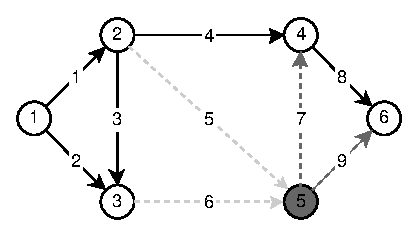
\includegraphics[width=\textwidth]{Chapter_I/7/1_7a.eps}
		\caption{}
	\end{subfigure}%
	\qquad
	\begin{subfigure}[b]{0.4\textwidth}
		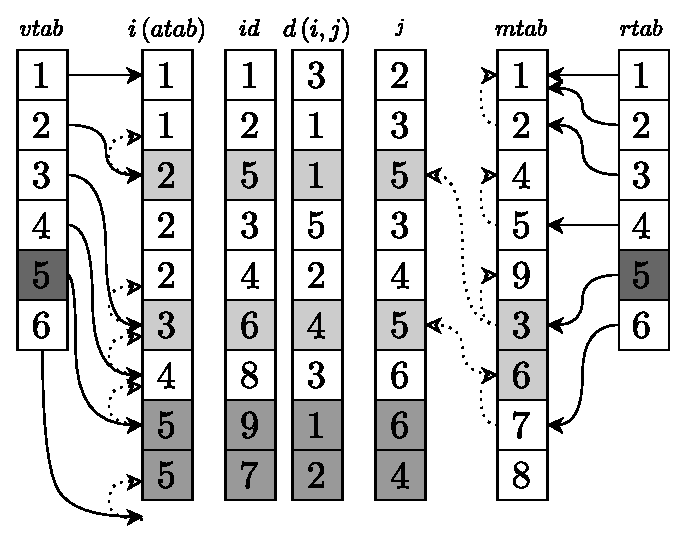
\includegraphics[width=\textwidth]{Chapter_I/7/1_7b.eps}
		\caption{}
	\end{subfigure}
	\caption{\textbf{Usunięcie węzła dla pęków wejścia-wyjścia} \textbf{(a)} Graf skierowany $G = \left( V, E \right)$. Usuwamy węzeł $v_{5}$ oraz wszystkie łuki wychodzące ($e_{7}, e_{9}$) i wchodzące do danego węzła ($e_{5}, e_{6}$). \textbf{(b)} Pęki z oznaczonymi łukami do usunięcia, wyznaczonymi odpowiednio w czasie $ O \left( A \left( 5 \right) \right)$ dla krawędzi wychodzących oraz $ O \left( A^{R} \left( 5 \right) \right)$ dla przychodzących. Węzeł, który należy usunąć wyznaczamy w czasie $ O \left( 1 \right)$. }
	\label{fig:forwardReverseStarRepresentationDeleteNode}
\end{figure}

\begin{figure}[!htbp]
	\ContinuedFloat
	\centering
	\begin{subfigure}[b]{0.4\textwidth}
		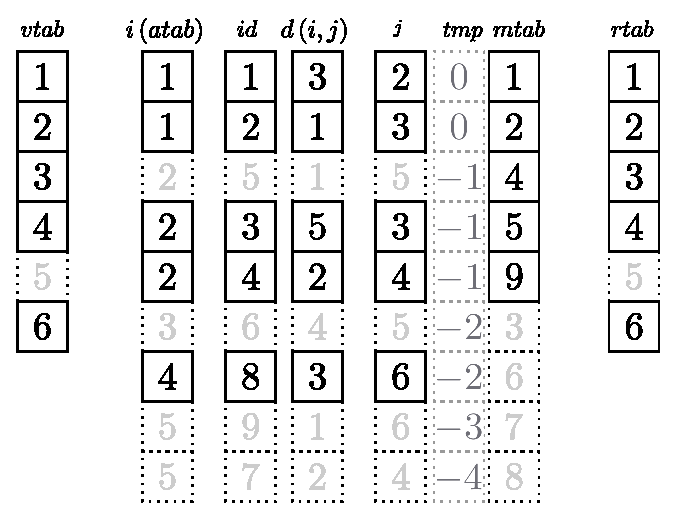
\includegraphics[width=\textwidth]{Chapter_I/7/1_7c.eps}
		\caption{}
	\end{subfigure}%
	\qquad
	\begin{subfigure}[b]{0.55\textwidth}
		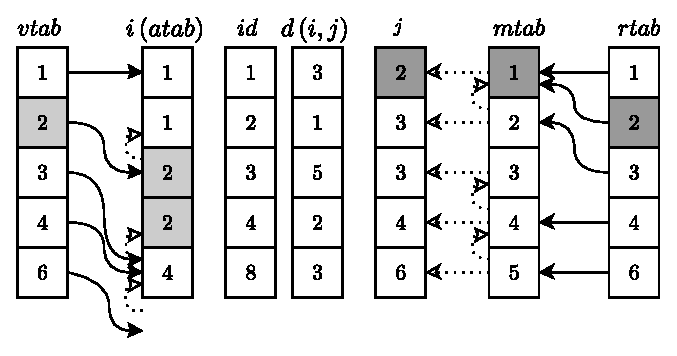
\includegraphics[width=\textwidth]{Chapter_I/7/1_7d.eps}
		\caption{}
	\end{subfigure}
	\caption{\textbf{(c)} Tablice z usuniętymi powiązaniami - po usunięciu chcianych elementów odtworzymy je w czasie liniowym. Rekonstrukcja związków, zachodzących między tablicami $vtab$, a $atab$ wymagać będzie przejścia przez ich wszystkie elementy, wyjąwszy krawędzie, wychodzące z ostatniego węzła, gdyż jego lista następników naturalnie kończy się wraz z końcem tablicy (po usunięciu wszystkich elementów tablice $vtab$ i $atab$ nadal będą prawidłowo posortowane). \textbf{(d)} Stan tablic po usunięciu węzła wraz z wszystkimi łukami. Odtworzenia własności tablicy $rtab$ oraz $mtab$ wymaga od nas większego nakładu pracy (ciąg wartości  \\ $j \left[ mtab \left[ 1 \right] \right], \ldots, j \left[ mtab \left[ \left| E \right| \right] \right] $ musi tworzyć ciąg niemalejący). W tym celu wprowadzamy pomocniczą tablicę, w której zapiszemy różnice indeksów elementów, jakie nastąpią w tablicy $j$ w trakcie usuwania krawędzi, a następnie aktualizujemy wszystkie elementy tablicy $mtab$ tak, aby $mtab \left[i \right] = mtab \left[i \right] + tmp \left[ mtab \left[ i \right] \right]$ (poza tymi, które wskazują na łuki, które będziemy usuwać - tutaj cztery ostatnie). \textbf{(d)} Sytuacja po usunięciu węzła $v_{5}$ i zaktualizowaniu wartości w tablicach. Szarym kolorem zaznaczono węzeł $v_{2}$ i powiązane z nim łuki.  }\label{fig:forwardReverseStarRepresentationDeleteNode1}
\end{figure}

W następnych rozdziałach spojrzymy już na sam problem najkrótszej ścieżki od strony zarówno formalnej jak i praktycznej - omówimy podstawowe własności problemu, zdecydujemy się na jeden ze, omówionych w powyższych rozdziałach, sposobów reprezentacji grafu, przedstawimy dodatkowe założenia, które ułatwią nam rozwiązanie problemu, jaki przed sobą postawiliśmy. Na koniec rozdziału - tak jak pisaliśmy na samym jego początku - przedstawimy krótko praktyczne zastosowanie zdobytej przez nas wiedzy w postaci algorytmu Bellmana-Forda.

\section{Problem najkrótszych ścieżek}
\label{sec:shortestPathProblem}

Omówiliśmy sposoby w jaki efektywnie możemy reprezentować dane, potrzebne nam do wyznaczenia najkrótszej ścieżki z punktu $v_{p}$ do węzła $v_{k}$ w skierowanym grafie z cyklami $G = \left( V, E \right)$, nie definiując przy tym formalnie samego problemu najkrótszej ścieżki, gdyż do tej pory, do opisu wszystkich reprezentacji grafu $G$, wystarczały nam intuicje, podparte prostą logiką. W dalszych rozważaniach będziemy opierać się o następujące oznaczenia i definicje:

\begin{myitemize}

\item \textbf{Ścieżką} od węzła $v_{p}$ do węzła $v_{k}$ będziemy nazywać każdą krawędź $e \in E$ w grafie $G = \left( V, E \right)$ taką, że ma ona swój początek w wierzchołku $v_{p} \in V$ i jest skierowana w stronę wierzchołka $v_{k} \in V$, gdzie ścieżka ta ma swój koniec. Z każdą ścieżką powiązana jest jej \textbf{waga} - dalej zwana również \textbf{kosztem} - $c_{pk}$, gdzie indeksy $p$ i $k$ odpowiadają indeksom węzłów: początkowego $v_{p}$ oraz końcowego $v{k}$, a którego wartość jest obliczana na podstawie, poniżej zdefiniowanej, \textbf{funkcji wagi}.

\item \textbf{Funkcja wagi} - jest funkcją, na podstawie której jest obliczany \textbf{koszt} danej ścieżki $e_{ij}$. W pseudokodach będziemy ją zwykle oznaczali przez $ d \left( v, u, \ldots \right) $, gdzie ostatni argument (,,$\ldots$'') oznacza, że \textbf{koszt} danej ścieżki może być zależny od wielu dodatkowych parametrów. My będziemy koszt każdej ścieżki $e_{ij}$ utożsamiać po prostu z jej długością i będziemy się do takiego kosztu odwoływać poprzez $c_{ij}$ (ang. \textit{cost}). Parametry funkcji $ d \left( v, u, c \right) $ będą kolejno oznaczały:

\begin{myitemize}

\item[v] - węzeł początkowy o indeksie $i$,
\item[u] - węzeł początkowy o indeksie $j$,
\item[c] - koszt $c_{ij}$ związany z łukiem $e_{ij}$, łączącym węzły $v$ i $u$.

\end{myitemize}


\item \textbf{Najkrótszą ścieżką} ze \textbf{źródła} $v_{p}$ do węzła $v_{k}$ nazywać będziemy takim zbiorem $P = \left \langle v_{0}, v_{1}, \ldots, v_{k} \right \rangle $, że suma kosztów $c_{ij}$ ścieżek jest najmniejsza:

\begin{equation}
\sum_{e_{ij} \in P^{'}} c_{ij} = minimum : e_{ij} \in P^{'} \Leftrightarrow v_{i},v_{j} \in P \: \wedge \: v_{i} \leadsto v_{j} = e_{ij} \ni E.
\end{equation}

gdzie przez $v_{i} \leadsto v_{j}$ będziemy oznaczać pojedynczą ścieżkę z węzła $v_{i}$ do węzła $v_{j}$. Wprowadzimy także zapis $v_{i} \overset{k}\leadsto v_{k}$, przez który będziemy rozumieć drogę złożoną z $k$ ścieżek, prowadzących od punktu $v_{i}$ do $v_{k}$ (użyty symbol ,,$*$''~ zamiast liczby ścieżek oznacza, że nie interesuje nas konkretna ich ilość, tylko fakt istnienia ścieżki o zadanych właściwościach - z danym punktem początkowym i końcowym). 

\item \textbf{Źródłem} $v_{S}$ będziemy nazywać węzeł, z którego rozpoczynamy wyszukiwanie najkrótszych ścieżek do wszystkich pozostałych węzłów w grafie i będzie to nasz podstawowy cel przy konstruowaniu wszystkich algorytmów, rozwiązujących problem najkrótszych ścieżek.

\end{myitemize}

\subsection{Reprezentacja problemu}
\label{sub:problemRepresentation}

Oprócz, omawianych już, własności naszej struktury oraz jej elementów składowych, takich jak koszt ścieżek $c_{ij}$, wspomnianych list sąsiedztwa, wprowadzimy także dodatkowe parametry dla węzłów, którymi będą:

\begin{myitemize}

\item \textbf{identyfikator węzła (ID)} jednoznacznie określa dany węzeł.

\item \textbf{poprzednik węzła (pred/$\Pi$)}, dalej zwany również jego \textbf{rodzicem}, który będzie determinował poprzedni węzeł na najkrótszej ścieżce (dla węzła $v_{i}$ będzie wyznaczał $v_{i-1}$ w $P = \left \langle v_{0}, v_{1}, \ldots, v_{i-1}, v_{i}, \ldots v_{k} \right \rangle $),

\item \textbf{waga najkrótszej ścieżki do węzła ($d \left( i \right) $)}, który dla węzła $v_{i}$ będzie przyjmował zawsze wartość najmniejszego znanego, kosztu przejścia ze źródła do tego węzła - dalej będziemy mówić o górnym ograniczeniu na koszt najkrótszej ścieżki, co okaże się równoważne (jeśli węzeł $v_{i}$ za wartość $ d \left( i \right) $ przyjmie $k$ to znaczy, że każda ścieżka $v_{S} \overset{*}\leadsto v_{i}$, aby być tą najkrótszą musi mieć łączny koszt nie większy niż $ d \left( i \right) $, czyli mniejszy lub równy $k$). Ponad to założymy, że dla każdego węzła $j$, do którego nie istnieje żadna ścieżka (w tym najkrótsza), bądź nie jest ona jeszcze znana, wartość $d \left( j \right) = \infty$ - wtedy dowolna ścieżka, która będzie nam pozwalała osiągnąć węzeł $j$ natychmiastowo stanie się najkrótszą ścieżką, do niego prowadzącą. Formalnie:

\begin{equation}
	d \left( i \right) \geqslant \delta \left ( s, i \right ) = \delta \left ( v_{s}, v_{i} \right ) = 
	\begin{cases}
	 \min \left\{ c \left( s,i \right ) : v_{s} \overset{*}\leadsto v_{i} \right\} & \text{ jeśli } \exists v_{s} \overset{*}\leadsto v_{i} \\ 
	 \infty & \text{ w przeciwnym przypadku }
	\end{cases}
\end{equation}

gdzie:

\begin{equation}\label{eq:sumCost}
c \left( p,k \right ) = c \left( v_{p}, v_{k} \right ) = \sum_{e_{ij} \in P} c_{ij} \; : \; P = \left \langle v_{p}, v_{1}, \ldots, v_{k} \right \rangle 
\end{equation}

\end{myitemize}

Do wszystkich atrybutów węzłów będziemy odwoływać się w dalszej części albo umieszczając jego nazwę w górnym indeksie, jak to robiliśmy do tej pory (np. $v{i}^{ID}$ oznaczał identyfikator węzła $i$ ), albo pisząc ją za operatorem kropki w przypadku, gdy górny indeks będzie potrzebny nam do czego innego (np. zapis $v_{i}^{ \left( k \right) }.\Pi$ będzie oznaczał $k$'tego rodzica \footnote{W sensie takim, że dla $k=1$ (domyślnie) wyrażenie $v_{i}^{ \left( k \right) }.\Pi$ oznacza rodzica podanego węzła, dla $k=2$ dziadka, dla $k=3$ pradziadka itd.} węzła $v_{i}$).

Aby efektywnie móc rozwiązywać problem najkrótszych ścieżek musimy przyjąć kilka założeń, które wynikają zarówno ze specyfikacji samego problemu, z przyjętego modelu (rzeczywistych sieci drogowych) oraz ograniczeń, jakie nakłada na nas konieczność reprezentacji wszystkich danych w sposób zrozumiały dla komputera.

Na samym początku należy wspomnieć o sposobie numerowania podstawowych elementów grafu $G = \left( V, E \right)$. Do tej pory milcząco zakładaliśmy, że każdy wierzchołek $v \in V$ w grafie $G$ ma przypisany swój własny, unikalny identyfikator, będący dodatnią liczbą całkowitą. Co więcej, identyfikatory te były przypisywane do tych wierzchołków w kolejności rosnącej ze skokiem o 1 tak, aby identyfikator ostatniego węzła równocześnie był liczbą wszystkich węzłów w grafie. Podobnie numerowaliśmy wszystkie krawędzie $e \in E$ - pozostaniemy przy tych oznaczeniach dla prostoty omawianego problemu, lecz nic nie stoi na przeszkodzie, by zamiast zwykłych tablic (bo temu właśnie ma służyć taka numeracja elementów grafu) wykorzystać bardziej złożone struktury, bądź \textit{tablice z haszowaniem}, które pozwoliłyby nam nazywać węzły dowolnie (mapując ich nazwy na liczby naturalne od $1$ do $ \left| V \right| $).

Bardziej restrykcyjnym założeniem o podobnym charakterze jest ograniczenie wartości wag wszystkich krawędzi (a co za tym idzie wag najkrótszych ścieżek w węzłach) do liczb całkowitych dodatnich. O ile jego obejście także nie stanowi większego problemu (wystarczy podnieść rząd wielkości wszystkich wartości tak, aby otrzymać liczby całkowite) to brak spełnienia tego warunku uniemożliwi nam efektywną konstrukcję pewnych wariantów algorytmów Dijkstry, które w dużej mierze opierają swoje działanie o te właśnie wartości (wspomniane algorytmy omówimy w rozdziale \ref{sec:dijkstraBuckets}). Dodatkowo w międzyczasie przemyciliśmy kolejne bardzo ważne założenie, które poczynimy - żadna z wag krawędzi w naszym grafie nie będzie mogła przybrać wartości ujemnej. Założenie to nie tylko jest słuszne z siecią drogową jako modelem, który sobie obraliśmy, lecz także bezpośrednio z niego wypływa inna własność, którą chcielibyśmy, aby miała nasza sieć - brak cykli o ujemnej długości tj. brak takich zamkniętych ścieżek, którymi da się przejść, a których koszt całkowity jest niedodatni ($ c \left( i, i \right) < 0 $, gdzie $v_{i}$ to odpowiednio ,,początek''~ i ,,koniec''~ cyklu). 

\begin{figure}[!htbp]
	\centering
	\begin{subfigure}[b]{0.45\textwidth}
		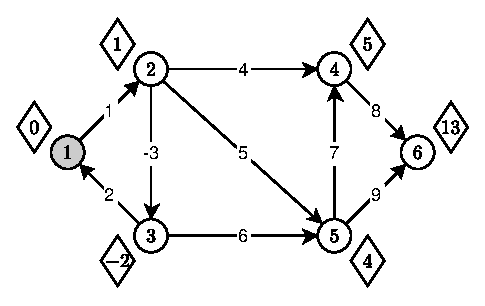
\includegraphics[width=\textwidth]{Chapter_I/8/1_8a.eps}
		\caption{}
	\end{subfigure}%
	\qquad
	\begin{subfigure}[b]{0.45\textwidth}
		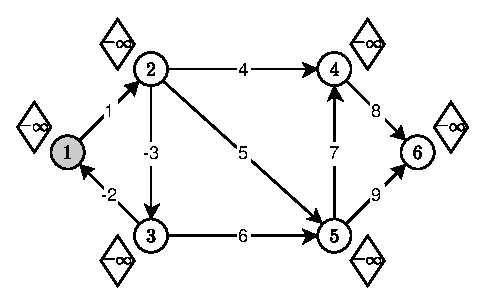
\includegraphics[width=\textwidth]{Chapter_I/8/1_8b.eps}
		\caption{}
	\end{subfigure}
	\caption{\textbf{Graf skierowany z ujemnymi wagami na krawędziach} \textbf{(a)} Węzeł $v_{1}$ jest źródłem, na krawędziach umieszczono ich wagi, a w rombach przy węzłach, do których prowadzą odpowiednio koszty najkrótszych ścieżek do tych węzłów ($d \left( 1 \right) = 0$). W samych węzłach umieszczono ich identyfikatory. Pomimo wystąpienia krawędzi $e_{23}$ o wadze $c_{23} < 0$ to długości najkrótszych ścieżek dla każdego z węzłów nadal są poprawnie wyliczone i przedstawiają faktyczny koszt najkrótszych ścieżek. \textbf{(b)} Wraz z pojawieniem się cyklu o ujemnej wadze ($v_{1} \leadsto v_{2} \leadsto v_{3} \leadsto v_{1} \leadsto \ldots$) wszystkie koszty w wierzchołkach stają się nieskończenie małe (z każdym kolejnym cyklem koszt dotarcia do węzłów w tym cyklu maleje, jednocześnie wpływając na koszt we wszystkich wierzchołkach, które są z tych węzłów osiągalne - dalej proces przebiega lawinowo, gdyż $- \infty + n = - \infty$). Oczywistym jest, że takie wyniki są dla nas bezwartościowe, gdyż informują co najwyżej o wystąpieniu w grafie ujemnego cyklu oraz o wierzchołkach, do których możemy dojść z jego wykorzystaniem.}\label{fig:negativeCycle}
\end{figure}

Jak pokazano na rysunku \ref{fig:negativeCycle}, za poprawną ścieżkę będziemy traktować tylko takie ścieżki, które nie zawierają w sobie cykli o ujemnej długości. Dodatkowo też za takie ścieżki będziemy uważać wszystkie, które zawierają cykl także o koszcie dodatnim (z analogicznego powodu). Załóżmy, że istnieje najkrótsza ścieżka $P = \left \langle v_{0}, v_{1}, \ldots, v_{k} \right \rangle $ taka, że $c \left( 0, k \right) = D$ i zawiera ona cykl dowolnej, niezerowej długości (powiedzmy $c = \left \langle v_{i}, v_{i+1}, \ldots, v_{j} \right \rangle $, gdzie $v_{i} = v_{j} $ oraz $c \left( i, j \right) \neq 0$). Nasza ścieżka zatem wygląda tak: $P = \left \langle v_{0}, v_{1}, \ldots, v_{i}, v_{i+1}, \ldots, v_{j}, \ldots, v_{k} \right \rangle $ (bez straty ogólności załóżmy, że cykl nie znajduje się na żadnym z końców ścieżki) i ma ona koszt $c \left( 0, k \right) = D$. Jeżeli chcielibyśmy usunąć teraz węzły cyklu od $v_{i+1}$ do $v_{j}$ to otrzymamy następującą ścieżkę: $P^{'} = \left \langle v_{0}, v_{1}, \ldots, v_{i}, v_{j+1}, \ldots, v_{k} \right \rangle $ o tym samym węźle początkowym i końcowym \footnote{Nie usuwamy pierwszego węzła cyklu, więc jeżeli cykl znajdowałby się na początku ścieżki to w oczywisty sposób węzeł $v_{p}$ na ścieżce $v_{p} \overset{*}\leadsto v_{k}$ nie uległby zmianie. Analogicznie w przypadku, gdyby cykl znajdował się na końcu tj. $P = \left \langle v_{0}, v_{1}, \ldots, v_{i}, v_{i+1}, \ldots, v_{j} \right \rangle $ i $v_{j}=v_{k}$, gdzie usunięcie cyklu spowodowałoby powstanie ścieżki  $P^{'} = \left \langle v_{0}, v_{1}, \ldots, v_{i} \right \rangle $. Pamiętając, że węzły $v_{i}$ oraz $v_{j}$ były odpowiednio początkiem i końcem cyklu $c$, a co za tym idzie: $v_{i} = v_{j} = v_{k} $.}, co poprzednia ścieżka (a więc ,,tą samą''~ ścieżkę), tyle że o zmienionym koszcie. Jeżeli usunęliśmy cykl o długości dodatniej, to nowa ścieżka będzie miała mniejszą wagę od ścieżki $P$, co czyni tą drugą dłuższą od $P^{'}$ - czyli ścieżka $P$ nie mogła być tą najkrótszą. Analogicznie możemy postępować dla cyklu o ujemnej długości, tyle że w tym przypadku zamiast usuwać cykle, będziemy je dodawać, by dojść do tej samej sprzeczności, co w poprzednio.

Z tego faktu dodatkowo wynika, że każda najkrótsza ścieżka może posiadać maksymalnie $\left| V \right| - 1$ składowych krawędzi - gdyby posiadała ich więcej, znaczyłoby to, że na ścieżce występuje cykl, a wykluczyliśmy już taką możliwość (nie zajmowaliśmy się cyklami długości zero, gdyż takie zawsze możemy eliminować z najkrótszych ścieżek).

Ostatnimi założeniami, jakie przyjmiemy, będą te związane z poprawną reprezentacją obliczeń, jakie będziemy wykonywać podczas wykonywania algorytmów (a które jedno już przedstawiliśmy). Jako, że dopuszczać będziemy sytuacje, w których dla danego węzła $v_{i}$ jego $v_{i}.d$ \footnote{$v_{i}.d \equiv v_{i}^{d} \equiv d \left( i\right)$} będzie się równać $- \infty$ albo $\infty$, konieczne jest zdefiniowanie operacji przy wykorzystaniu tych symboli nieoznaczonych. W związku z tym, będziemy przyjmować, że dla dowolnej liczby $n \neq \pm \infty$ zachodzić będą równości: $ a + \left( \mp \infty \right) = \left( \mp \infty \right) + a = \mp \infty$.

W dalszej części, przy omawianiu algorytmów, będziemy posługiwać się jedną z, przedstawionych wcześniej, reprezentacji grafu - w naszym przypadku będą to listy sąsiedztwa, gdyż w najbardziej naturalny (a zarazem najprostszy) sposób wyrażają one wszystkie własności, z jakich przyjdzie nam korzystać podczas konstruowania algorytmów wyszukiwania najkrótszych ścieżek.

\subsection{Podstawowe operacje}

Omówimy teraz podstawowe operacje, z których będziemy bardzo często korzystać w trakcie budowania kolejnych algorytmów wyszukujących najkrótsze ścieżki.

Jedną z takich operacji jest niewątpliwie procedura inicjalizująca graf, na którym dany algorytm będzie pracować. Jak wspomnieliśmy w poprzednich rozdziałach, w przypadkach, gdy nie istnieje najkrótsza ścieżka, bądź nie mamy informacji o takowej, która by prowadziła do danego węzła $i$, wtedy wartość parametru tego węzła $d \left( i \right) = \infty$ - przed rozpoczęciem działania algorytmu o ścieżkach nie wiemy nic, zatem każdy wierzchołek inicjalizujemy w ten sposób, dodatkowo upewniając się, że żaden z nich nie posiada informacji o swoim rodzicu (jako, że takie informacje posłużą nam później do odtworzenia znalezionych, najkrótszych ścieżek). Źródło $v_{S}$ - wierzchołek w grafie, od którego zaczniemy poszukiwania najkrótszych ścieżek - będzie miało ustawiony dystans ($d \left( S \right)$) na wartość równą zeru (,,najkrótszą ścieżką'' do węzła $v_{S}$ z węzła $v_{S}$ jest ścieżka długości zero - założyliśmy brak ujemnych cykli oraz brak jakichkolwiek krawędzi o takim koszcie).

\begin{algorithm}[!htbp]
\DontPrintSemicolon
\Begin{
	\For(\tcc*[f]{Dla każdego węzła w $vtab$}){$vIdx\in 1 \ldots \left| V \right| $}{
		$vtab \left[ vIdx \right].d \longleftarrow \infty$\; 
		$vtab \left[ vIdx \right].\Pi \longleftarrow \KwNull$\; 
	}
	$vtab \left[ s \right].d \longleftarrow 0$\; 
}
\caption{INIT-GRAPH $\left( G, s \right)$\label{alg:init-graph}}
\end{algorithm}

Dwa rozdziały temu wprowadziliśmy kilka nowych oznaczeń dla atrybutów węzłów, z których od tamtej pory mieliśmy korzystać. Mówiliśmy, że dla każdego węzła $v_{i}$ jego wartość $d \left( i \right) $ przyjmuje zawsze koszt równy najmniejszemu, znanemu kosztowi ścieżki, prowadzącej ze źródła do danego węzła , co formalnie możemy w skróconej formie wyrazić:

\begin{equation}
d \left( i \right) = \sum_{e_{jk} \in P} c_{jk} \rightarrow min\; : \; P = \left \langle e_{Sj^{ \left( 1 \right) }}, e_{j^{ \left( 1 \right) } j^{ \left( 2 \right) }}, \ldots, e_{j^{ \left( m \right) } i } \right \rangle
\end{equation}

gdzie $P$ jest zbiorem krawędzi dla istniejącej ścieżki $v_{S} \overset{m+1}\leadsto v_{i}$.

W czasie działania wszystkich algorytmów wyszukiwania najkrótszych ścieżek będziemy chcieli zachować tę własność, by w momencie zakończenia ich działania otrzymywać poprawne wyniki (czyli by $\forall v \in V \; d \left( i \right) = \delta \left( s, i \right)$). Aby to było możliwe, musimy wprowadzić kolejną operację, którą będziemy nazywać operacją relaksacji krawędzi. Przyjrzyjmy się sytuacji, która zobrazuje jej działanie.

\begin{figure}[!htbp]
	\centering
	\begin{subfigure}[b]{0.45\textwidth}
		
\includegraphics[width=\textwidth]{Chapter_I/9/1_9a.eps}
		\caption{}
		\label{fig:relaxEdges:a}
	\end{subfigure}%
	\qquad
	\begin{subfigure}[b]{0.45\textwidth}
		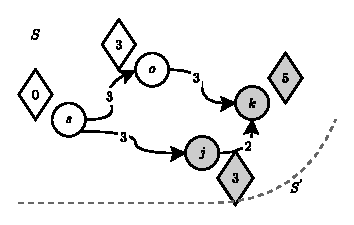
\includegraphics[width=\textwidth]{Chapter_I/9/1_9b.eps}
		\caption{}
		\label{fig:relaxEdges:b}
	\end{subfigure}
	\caption{\textbf{Relaksacja krawędzi} \textbf{(a)} Sytuacja przed dodaniem wierzchołka $v_{j}$ do zbioru wierzchołków o optymalnych wartościach $d \left( i \right) $, gdzie $i \in \left\{ i^{'} : v_{i^{'}} \in S \right\} $. \textbf{(b)} Dodanie do zbioru $S$ wierzchołka $v_{j}$ spowodowało powstanie nowej ścieżki $v_{s} \overset{*}\leadsto v_{k}$, której koszt jest mniejszy od dotychczasowej $v_{s} \leadsto v_{o} \leadsto v_{k}$ i w efekcie reorganizację najkrótszej ścieżki węzła $v_{k}$. Etykieta $ d \left( k \right)$ uległa zmniejszeniu, a $v_{k}.\Pi$ wskazuje teraz na węzeł $v_{j}$ (poprzednio $v_{o}$).}\label{fig:relaxEdges}
\end{figure}

Na rysunku \ref{fig:relaxEdges} przedstawiona jest sytuacja w trakcie działania pewnego algorytmu wyszukiwania najkrótszych ścieżek, gdzie wyszarzono wszystkie wierzchołki (oraz powiązane z nimi krawędzie), o których algorytm jeszcze nic nie wie (przyjmijmy, że zbiór tych wierzchołków będziemy oznaczać krótko jako $S^{'}$ - rys. \ref{fig:relaxEdges:a}), gdyż zaczął je przeglądać od danego węzła $v{S}$ - źródła. W tej chwili wszystkie atrybuty $d \left( i \right)$ węzłów nie należących do zbioru $S^{'}$ (nazwijmy go zbiorem $S$) mają wartości, odpowiadające kosztom najkrótszych ścieżek od źródła do każdego z nich (są optymalne) i jest to sytuacja, którą chcemy utrzymać. Przyjmijmy teraz, że do zbioru wierzchołków $S$ dołączamy wierzchołek $v_{j} \in S^{'}$ (jednocześnie go stamtąd usuwając - rys. \ref{fig:relaxEdges:b}). Po dodaniu wierzchołka $v_{j}$ widzimy, że do $v_{k}$ da się dojść krótszą ścieżką, niż to było przedstawione na rysunku \ref{fig:relaxEdges:a}, a zatem $d \left( k \right)$ nie jest już długością najkrótszej ścieżki dla tego węzła. Podobnie węzeł $v_{o} = v_{k}^{\Pi}$ nie należy już do zbioru węzłów, leżących na najkrótszej ścieżce $v_{S} \overset{*}\leadsto v_{k}$. Łatwo zauważyć, że jedyną możliwą alternatywą dla najkrótszej ścieżki do węzła $v_{k}$ jest przed chwilą powstała ścieżka, tak więc nowa wartość parametru $d \left( k \right) = min \left\{ d \left( o \right) + c_{ok}, d \left( k \right) \right\} $ \footnote{O tym, że tak jest w istcie przekonamy się w następnym rozdziale.}.

\begin{algorithm}[!htbp]
\DontPrintSemicolon
\Begin(\tcc*[f]{Oznaczenia węzłów zachowane z rysunku \ref{fig:relaxEdges}}){
	\If(\tcc*[f]{$d \left( j, k, \ldots \right)$ - funkcja wagi}){$ k.d > j.d + d \left( j, k \right)$} {
		$ k.d \longleftarrow j.d + d \left( u, k \right)$ \;
		$ k.\Pi \longleftarrow j$ \;
	}
}
\caption{RELAX $\left( j, k, d \right)$ \label{alg:relax}}
\end{algorithm}

Algorytm relaksacji wierzchołków sprawdza, czy nowo dodany wierzchołek zaburza, interesującą nas, własność grafu. Jeżeli nie to następne kroki są pomijane. W przeciwnym przypadku aktualizowane jest wskazanie na rodzica $d$ oraz wartość $d \left( i \right)$  dla wierzchołka, który tego wymaga. Metoda relaksacji przyjmuje trzy parametry, z którego dwa są wierzchołkami, a trzeci funkcją wagową krawędzi, którą zdefiniowaliśmy w podrozdziale \ref{sec:shortestPathProblem}.

Ostatnią operacją, którą chcielibyśmy móc wykonywać jest operacja przeglądania wierzchołków, które znajdują się na dowolnej najkrótszej ścieżce w grafie $G = \left( V, E \right)$, jako że sama informacja o długości takiej ścieżki nie zawsze okazuje się wystarczająca. Przy omawianiu dwóch poprzednich algorytmów na równi z operowaniem na atrybutach węzłów $d \left( i \right)$ pozwalaliśmy sobie zmieniać także atrybut, odpowiadający wskazaniu na rodzica danego węzła ($\Pi$), doprowadzając zawsze do sytuacji, w której rodzicem danego węzła, leżącego na najkrótszej ścieżce, zawsze był węzeł, który także na niej się znajdował, będąc jednocześnie o jedną krawędź bliżej źródła, od którego dana ścieżka się rozpoczynała. Innymi słowy dbaliśmy o to, by dla każdej najkrótszej ścieżki $ P = \left \langle v_{0}, v_{1}, \ldots, v{k} \right \rangle$ dla każdego $v_{i} : i \in \left\{ 1, \ldots, k \right\}$ zachodziła prawidłowość: $v_{i}.\Pi = v_{i-1}$ (dla $i = 0$ w oczywisty sposób $v_{0}.\Pi = \KwNull$), a zatem nasz algorytm, pozwalający nam na wypisanie po kolei węzłów na danej, najkrótszej ścieżce $v_{0} \overset{k} \leadsto v_{k}$, wyglądać mógłby dla przykładu tak:

\begin{algorithm}[!htbp]
\DontPrintSemicolon
\KwResult{Ścieżka, wypisane w kolejności od węzła docelowego do źródła.}
\Begin{
	\While{$ v.\Pi \neq \KwNull $} {
		Wypisz $v$ \;
		$  v \longleftarrow v.\Pi$ \;
	}
	Wypisz $v$ \;
}
\caption{WRITE-PATH $\left( v \right)$ \label{alg:writePAth}}
\end{algorithm}

gdzie na wejściu musielibyśmy podać węzeł, do którego ścieżkę chcemy wypisać, pamiętając, że będzie to ścieżka wypisana w odwrotnej kolejności i że nie jesteśmy w stanie wypisać najkrótszych ścieżek innych, niż te, które swój początek mają w źródle (zbiór wszystkich takich ścieżek tworzy swego rodzaju drzewo, którego korzeniem jest właśnie ten węzeł - rys. \ref{fig:shortestPathTree}).

\begin{figure}[!htbp]
	\centering
	\begin{subfigure}[b]{0.45\textwidth}
		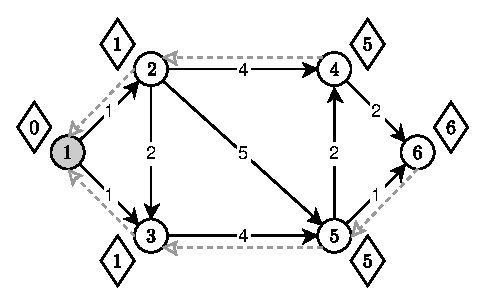
\includegraphics[width=\textwidth]{Chapter_I/10/1_10a.eps}
		\caption{}
	\end{subfigure}%
	\qquad
	\begin{subfigure}[b]{0.45\textwidth}
		
\includegraphics[width=\textwidth]{Chapter_I/10/1_10b.eps}
		\caption{}
	\end{subfigure}
	\caption{\textbf{Poddrzewo najkrótszych ścieżek} \textbf{(a)} Graf $G = \left( V, E \right)$ z obliczonymi odległościami najkrótszych ścieżek dla wszystkich węzłów, gdzie przerywanymi liniami zaznaczone są wskazania na poprzedników każdego z nich. W przypadku braku takiej krawędzi dla danego węzła $v$ zakładamy, że $v.\Pi = \KwNull$. \textbf{(b)} Poddrzewo grafu, zawierające najkrótsze ścieżki od źródła do wszystkich pozostałych węzłów w grafie $G$, w raz z ich kosztami.}\label{fig:shortestPathTree}
\end{figure}

Oczywiście nic nie stoi na przeszkodzie, byśmy zastosowali jedną z technik, by odwrócić kolejność takiego wypisywania (np. wpisać wyniki do kolejki FIFO, by później z niej odczytać wartości w kolejności od $v_{0}$ do $v_{k}$ czy też zastosować rekursję).

\subsection{Właściwości najkrótszych ścieżek}
\label{sub:shortestPathProperties}

Algorytmy, które będziemy omawiać w następnych rozdziałach, poza czerpaniem pomysłów na ich implementacje z wielu innych zagadnień informatycznych (jak się przekonamy), w głównej mierze oparte będą na właściwościach najkrótszych ścieżek, które przytoczymy w tym podrozdziale bez dowodów (Czytelnik może je wszystkie odnaleźć w dodatku TODO), wierząc, że pomoże się to skupić Czytelnikowi na samych algorytmach i dowodach ich poprawności, zwłaszcza, że zdecydowana większość właściwości najkrótszych ścieżek jest naturalna i łatwa do zrozumienia.

\begin{lemma}[Własność trójkąta]\label{lem:triangleInequality}
Dla każdej krawędzi $e_{ij} \in E$ w zachodzi $ \delta \left( v_{k}, v_{j} \right) \leqslant \delta \left( v_{k}, v_{i} \right) + c_{ij}$.
\end{lemma}

\begin{lemma}[Własność optymalnej podstruktury]\label{lem:optimalSubstructure}
Jeśli w ważonym grafie skierowanym $ G = \left( V, E \right)$ z funkcją wagową $w: E \leftarrow \RR$ (w naszym przypadku wagi są utożsamiane z kosztem przejścia między jednym węzłem, a drugim, wyrażonym - bez straty ogólności - w liczbach naturalnych, gdyż zajmujemy się rzeczywistymi sieciami drogowymi, w których odległości między dowolnymi dwoma punktami mierzymy w całkowitych wielokrotnościach przyjętej jednostki długości) najkrótszą ścieżką z wierzchołka $v_{p}$ do $v_{k}$ jest ścieżka $P = \left \langle v_{p}, v_{p+1}, \ldots, v_{k} \right \rangle $ to dla każdych $i,j$ takich, że $p \leqslant i \leqslant j \leqslant k$ podścieżka $P_{ij} = \left \langle v_{i}, v_{i+1}, \ldots, v_{j} \right \rangle $ jest najkrótszą ścieżką z $v_{i}$ do $v_{j}$.
\end{lemma}

\begin{lemma}[Własność braku ścieżki]\label{lem:noPath}
Jeśli nie istnieje ścieżka z $s$ do $v_{i}$ to zawsze $v_{i}.d = \delta \left( s, i \right) = \infty$
\end{lemma}

\begin{lemma}[Własność ścieżki z ujemnym cyklem]\label{lem:pathWithNegativeCycle}
Jeśli istnieje ścieżka $P = \left \langle v_{p}, v_{p+1}, \ldots, v_{k} \right \rangle $ z $v_{p}$ do $v_{i}$, na której znajduje się cykl o ujemnej wadze $P = \left \langle v_{i}, v_{i+1}, \ldots, v_{j} \right \rangle $, gdzie $p \leqslant i \leqslant j \leqslant k$ to zawsze $v_{k}.d = \delta \left( p, k \right) = - \infty$
\end{lemma}

\begin{lemma}[Własność górnego ograniczenia]\label{lem:costUpperBound}
Dla każdego wierzchołka $v_{i} \in V$ zachodzi $ v_{i}.d \geqslant \delta \left( s , v_{i} \right)$, gdzie wartość $v_{i}.d$ monotonicznie maleje i w momencie osiągnięcia swojego dolnego ograniczenia $\delta \left( s , v_{i} \right)$ przestaje ulegać zmianie.
\end{lemma}

\begin{lemma}[Własność zbieżności]\label{lem:convergenceProperty}
Jeśli w grafie ważonym $G = \left( V, E \right)$ istnieje najkrótsza ścieżka $P = \left \langle v_{p}, v_{p+1}, \ldots, v_{k-1}, v_{k} \right \rangle $ i w dowolnym momencie przed relaksacją krawędzi $e_{kk-1}$ zachodzi $ v_{k-1}.d = \delta \left( v_{p}, v_{k-1} \right)$ to po tej relaksacji $ v_{k}.d = \delta \left( v_{p}, v_{k} \right)$.
\end{lemma}

\begin{lemma}[Własność relaksacji dla ścieżki]\label{lem:pathRelaxation}
Jeśli $P = \left \langle v_{p}, v_{p+1}, \ldots, v_{k} \right \rangle $ jest najkrótszą ścieżką z $s = v_{p}$ do $v_{k}$ i wykonamy szereg relaksacji jej krawędzi w kolejności od $e_{pp+1}$ do $e_{k-1k}$ to $v_{k}.d$ będzie równe $ \delta \left( s, v_{k}\right)$ niezależnie od kolejności wykonywania pozostałych relaksacji.
\end{lemma}

\begin{lemma}[Własność podgrafu poprzedników]\label{lem:parentSubgraph}
Jeśli dla każdego węzła $v_{i}$ w grafie $G = \left( V, E \right)$ zachodzi $v_{i}.d = \delta \left( s, v_{i} \right)$ to podgrafem poprzedników grafu $G$ jest drzewo o korzeniu w węźle $s$ i krawędziach, będących odwzorowaniem wszystkich najkrótszych ścieżek w tym grafie.
\end{lemma}

\subsection{Algorytm Bellmana-Forda}

Ostatnim naszym krokiem w tym rozdziale będzie przedstawienie prostego algorytmu, wykorzystującego całą naszą, dotychczas zdobytą, wiedzę, do wyznaczenia najkrótszych ścieżek w zadanym, skierowanym grafie acyklicznym $G = \left( V, E \right)$ z nieujemnymi wagami na krawędziach. Algorytm, o którym będziemy mówić w tym rozdziale, jest oparty na właściwościach najkrótszych ścieżek, które omówiliśmy powyżej i bezpośrednio z nich wynika dowód jego poprawności, który także przytoczymy. Bardzo prostą ideą omawianego algorytmu jest wykonanie operacji relaksacji krawędzi w rundach aż ,,do skutku''. Pod pojęciem rundy będziemy rozumieli przeprowadzenie takiej operacji dla każdej krawędzi w grafie dokładnie jeden raz, zaś wykonywanie rund będziemy powtarzać do momentu, w którym wartości $ d \left( i \right) $ każdego wierzchołka $V_{i}$ w grafie osiągną wartości równych rzeczywistym wagom najkrótszych ścieżek $v_{s} \overset{*}\leadsto v_{i}$ - dalej, dla zachowania prostoty, będziemy te wartości zapisywać w skrócie jako: $ \delta \left( s, i \right)$. Naszym celem zatem staje się już tylko znalezienie takiej minimalnej ilości rund, po których dla każdego wierzchołka $ v_{i} \in G $ zachodzi równość $ d \left( i \right) = \delta \left( s, i \right) $ (dla źródła $ s $). W tym momencie warto przypomnieć sobie, że w naszym modelu rzeczywistych sieci drogowych przyjęliśmy brak krawędzi, których koszt byłby mniejszy lub równy $ 0 $, a co za tym idzie najkrótsze ścieżki, które będziemy chcieli odnaleźć, nie będą składać się z więcej niż $ \left| V \right| - 1 $ elementów i przechodzić przez więcej niż  $ \left| V \right| -2 $ wierzchołków, nie wliczając to wierzchołka początkowego i końcowego - zwróciliśmy już uwagę na tę własność najkrótszych ścieżek pod koniec podrozdziału \ref{sub:problemRepresentation}.

\begin{algorithm}[!htbp]
\DontPrintSemicolon
\Begin{
	\For{$i = 1$ \emph{\KwTo} $ \left| V \right| - 1$}{
		\ForAll{$ \left( u, v \right) \in E$}{
		$RELAX \left( u, v \right)$ \;
		}
	}
	\ForAll{$ \left( u, v \right) \in E$}{
		\If{$ v.d > u.d + c_{uv}$}{
			\Return \KwFalse \;
		}
	}
	\Return \KwTrue \;
}
\caption{ BELLMAN-FORD $\left( G, s \right)$\label{alg:BellmanFord}}
\end{algorithm}

Powyżej została przedstawiona podstawowa wersja algorytmu Bellmana-Forda, której pesymistyczna złożoność, jeżeli chodzi o ilość wykonywanych operacji, da się w oczywisty sposób oszacować przez $ O \left( \left| V \right| \cdot \left| E \right| \right) $ - wykonujemy $ O \left( \left| V \right| \right) $ razy instrukcje $ \left( 3 \right) = \left( 4 \right) $, gdzie każda z nich wykonuje dokładnie $ \left| V \right| $ operacji \textsf{RELAX}. Druga pętla, którą widzimy, przegląda raz jeszcze wszystkie krawędzie w grafie, upewniając się, że nie można wykonać na którejkolwiek z nich dodatkowej relaksacji, czyli innymi słowy - czy nasz algorytm zakończył swoje działanie i dał poprawny wynik. Jeżeli po wykonaniu pierwszej z pętli znajdziemy taką krawędź $ \left( u, v \right) \in E $, że spełniony będzie warunek $ v.d > u.d + c_{uv}$ to niechybny znak, że w gafie, w którym szukaliśmy najkrótszych ścieżek od źródła $s$ do wszystkich pozostałych węzłów, występuje cykl o ujemnej długości. Do takiego wniosku dojdziemy, wykonując proste rozumowanie:

Załóżmy, że mamy w grafie cykl $C = \left \langle v_{0}, v_{1}, \ldots, v_{k} \right \rangle $, gdzie $ v_{0} = v_{k}$, a ponadto, że - mimo jego występowania - algorytm po wykonaniu drugiej pętli zwróci nam wartość pozytywną \textsf{\KwTrue} (czyli, że dla każdej krawędzi $ \left( u, v \right) \in E $ zaszła nierówność $ v.d \leqslant u.d + c_{uv}$ w tym i dla wszystkich krawędzi, należących do cyklu). Jak wspomnieliśmy w podrozdziale \ref{sub:problemRepresentation}, cyklem ujemnym nazywamy taką zamkniętą ścieżkę, po której jesteśmy w stanie przejść, a całkowity koszt przejścia po wszystkich krawędziach tego cyklu wynosi $ c \left( v_{0}, v_{k} \right) < 0 $ (nierówność \ref{eq:sumCost}). Dokładniej:

\begin{equation}
\exists C = \left \langle v_{0}, v_{1}, \ldots, v_{k} \right \rangle \; \wedge \; v_{0} = v_{k} \; \wedge \; \sum _{i=1}^{k} c \left( v_{i-1}, v_{i} \right ) = c \left( v_{0} , v_{k} \right) < 0 \Leftrightarrow C - \textrm{cykl o ujemnej długości}
\end{equation}

Kluczową dla naszego rozumowania okaże się nierówność $\sum _{i=0}^{k-1} c \left( v_{i}, v_{i+1} \right ) < 0$ oraz fakt, że z definicji cyklu $v_{0} = v_{k}$ gdzie $v_{0}, v_{k} \in C$. Z założenia, że algorytm Bellmana-Forda zwraca wartość \textsf{\KwTrue} mamy $\forall_{v_{i} \in C} \; v_{i}.d \leqslant v_{i-1}.d + c_{v_{i-1}v_{i}}$, gdzie sumując po $v_{1}, \cdots, v_{k} \in C$ otrzymujemy:

\begin{equation}
\sum _{i=1}^{k} v_{i}.d \; \leqslant \; \sum _{i=1}^{k} \left( v_{i-1}.d + c_{v_{i-1}v_{i}} \right) = \sum _{i=1}^{k} v_{i-1}.d + \sum _{i=1}^{k} c \left( v_{i-1}, v_{i} \right ) = \sum _{i=1}^{k} v_{i-1}.d + c \left( v_{0} , v_{k} \right)
\end{equation}.

Z własności cyklu: $v_{0} = v_{k}$ możemy wyprowadzić taki ciąg równości:

\begin{equation}
\sum _{i=0}^{k} v_{i}.d = v_{0}.d + \sum _{i=1}^{k-1} v_{i}.d + v_{k}.d = \sum _{i=1}^{k} v_{i-1}.d + v_{k}.d = v_{0}.d + \sum _{i=1}^{k} v_{i}.d
\end{equation}

zaś z obu wyprowadzeń w ostateczności otrzymujemy:

\begin{gather*}
\sum _{i=1}^{k} v_{i}.d \; \leqslant \; \sum _{i=1}^{k} v_{i-1}.d + c \left( v_{0} , v_{k} \right) \\
\sum _{i=1}^{k} v_{i}.d = \sum _{i=1}^{k} v_{i-1}.d \\
0 \; \leqslant \; c \left( v_{0} , v_{k} \right)
\end{gather*}

co stoi w sprzeczności z tym, że na naszej ścieżce znajduje się cykl o ujemnej długości ($ c \left( v_{0}, v_{k} \right) < 0 $). Widzimy więc, że algorytm Bellmana-Forda, podobnie zresztą jak wszystkie, omawiane w tej pracy algorytmy, nie radzi sobie z wyszukiwaniem najkrótszych ścieżek w grafach, gdzie występują cykle o długości ujemnej (jak pokazaliśmy na przykładzie \ref{fig:negativeCycle}).

Sam zaś algorytm można nieco usprawnić, by nie wykonywał niepotrzebnych operacji i przez to działał szybciej od swojego pierwowzoru. Nie są to jednak zmiany na tyle duże, by miały jakikolwiek wpływ na pesymistyczną złożoność algorytmu.

\begin{figure}[!htbp]
	\centering
	\begin{subfigure}[b]{0.24\textwidth}
		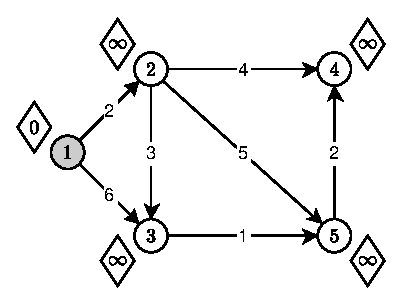
\includegraphics[width=\textwidth]{Chapter_I/11/1_11a.eps}
		\caption{}
	\end{subfigure}%
	\begin{subfigure}[b]{0.24\textwidth}
		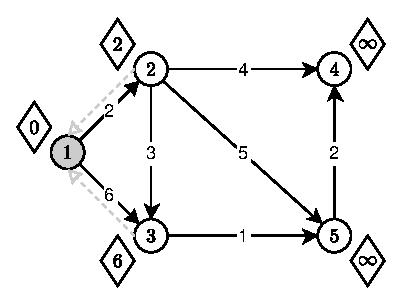
\includegraphics[width=\textwidth]{Chapter_I/11/1_11b.eps}
		\caption{}
	\end{subfigure}
	\begin{subfigure}[b]{0.24\textwidth}
		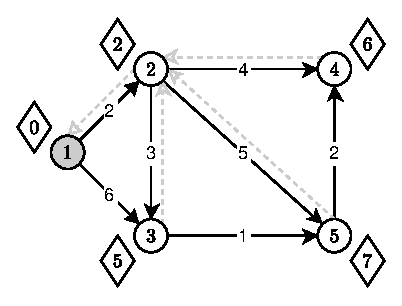
\includegraphics[width=\textwidth]{Chapter_I/11/1_11c.eps}
		\caption{}
	\end{subfigure}%
	\begin{subfigure}[b]{0.24\textwidth}
		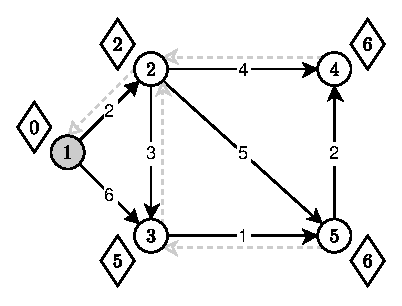
\includegraphics[width=\textwidth]{Chapter_I/11/1_11d.eps}
		\caption{}
		\label{fig:exampleBellmanFord:d}
	\end{subfigure}
	\caption{\textbf{Działanie algorytmu Bellmana-Forda} \textbf{(a)} Sytuacja po zainicjowaniu grafu $G = \left( V, E \right)$ przez \textsf{INIT-GRAPH} ze źródłem $v_{s}.id = 1$. \textbf{(b)} Warunek $ v.d > u.d + c_{uv} $ dla krawędzi $ \left( u, v \right) $ spełniony jest tylko dla krawędzi: $ \left( 1, 2 \right) $ i $ \left( 1, 3 \right) $ i dla tych węzłów ( $v_{2}$ i $v_{3}$ ) zostały zaktualizowani ich poprzednicy (zaznaczeni szarymi strzałkami) oraz etykiety $d$. Dla pozostałych algorytm nie wprowadził żadnych zmian w trakcie iterowania po wszystkich $ A \left( i \right) : i \in \left\{ 1, \ldots, 5\right\}$. \textbf{(c)} Przyjęliśmy kolejność iterowania po wszystkich łukach (pętla $3-4$) zgodną z kolejnością ponumerowania węzłów na rysunkach. Przyjmijmy ponadto rosnącą kolejność identyfikatorów węzłów, do której łuki prowadzą tj. podczas drugiej iteracji algorytm wykonuje operację \textsf{RELAX} na krawędziach w kolejności: $ \left( 1, 2 \right) $, $ \left( 1, 3 \right) $ (dla których relaksacja nie wprowadzi żadnych zmian), $ \left( 2, 3 \right) $ (zostaje zaktualizowany węzeł $v_{3}$ - jego wartość $d$ przyjmie długość odnalezionej, krótszej ścieżki oraz otrzyma nowego rodzica), $ \left( 2, 4 \right) $, $ \left( 2, 5 \right) $, \textbf{(d)} $ \left( 3, 5 \right) $ i $ \left( 5, 2 \right) $. Dla normalnej wersji algorytmu powinniśmy wykonać jeszcze 3 iteracje (z $ \left| V \right| - 1 $) po wszystkich krawędziach, jednak wprowadziliśmy modyfikację, która przerywa działanie algorytmu, jeżeli podczas pełnej iteracji nie nastąpi w grafie $G$ żadna zmiana.} \label{fig:exampleBellmanFord}
\end{figure}

\subsubsection{Usprawnienie algorytmu}

Pierwsze co możemy zauważyć to fakt, że jeśli uporządkujemy wszystkie krawędzie $e_{ij}$ względem pierwszego indeksu (czyli tak, aby kolejność przeglądania łuków w wierszach 3-4 była podyktowana przeglądanymi węzłami, z których dane łuki wychodzą) to możemy pomijać relaksacje tych wszystkich krawędzi, które wychodzą z węzła $v$, do którego jeszcze nie ma wyznaczonej ścieżki ($v.d = \infty$), gdyż warunek na jej wykonanie nigdy nie zajdzie ($ k.d > \infty + d \left( j, k \right)$). W wybranym przez nas sposobie prezentowania danych grafu (jako listy sąsiedztwa) taka kolejność przeglądania krawędzi jest naturalna (chcąc przejść przez wszystkie krawędzie w grafie będziemy kolejno przeglądać zawartość list $ A \left( i \right) : v_{i} \in G$). Dodatkowo - jak już zaznaczono na rysunku \ref{fig:exampleBellmanFord:d} - jeżeli w czasie wykonywania relaksacji wszystkich krawędzi w grafie nie nastąpi żadna zmiana to nie wystąpią one także podczas następnych iteracji głównej pętli algorytmu, a zatem możemy jej wykonanie przerwać, nie czekając aż wykona się ona dokładnie $ \left| V \right| - 1$ razy.

\subsubsection{Poprawność działania}

Dowód poprawności działania takiego algorytmu dla grafu $G = \left( V, E \right)$, który nie zawiera ujemnych cykli (dla których pokazaliśmy już, że omawiany algorytm nie działa) jest natychmiastowy, jeżeli powołamy się na odpowiednie własności najkrótszych ścieżek.

Z lematu \ref{lem:pathRelaxation} wiemy, że jeśli w grafie istnieje najkrótsza ścieżka $P = \left \langle v_{p}, v_{p+1}, \ldots, v_{k} \right \rangle $ i wykonamy dla jej krawędzi relaksację w odpowiedniej kolejności to $v_{k}.d$ będzie się równać $ \delta \left( s, v_{k} \right)$. Wiemy także, że każda najkrótsza ścieżka w grafie składać się może maksymalnie z $ \left| V \right| - 1 $ krawędzi. Z każdym nawrotem pętli głównej algorytmu Bellmana-Forda wykonywana jest relaksacja wszystkich krawędzi w grafie $G$, zaś pętla ta jest powtarzana dokładnie $ \left| V \right| - 1 $ razy. Podczas każdej $i$-tej iteracji w szczególności wykonamy relaksację dla wszystkich krawędzi na ścieżce $P$, a zwłaszcza dla $e_{pp+1}$ (w pierwszej iteracji), dla $e_{p+1p+2}$ i dla każdej następnej. W najgorszym przypadku, zależnym od faktycznej kolejności przeglądania krawędzi, ostatnią z nich na ścieżce $P$ będziemy relaksować w iteracji $k-p+1$ (w przypadku, gdy dla $k$ pierwszych $i$-tych iteracji $i = 1, 2, \cdots \left| V \right| - 1$ będziemy wykonywali relaksację tylko jednej krawędzi ze ścieżki $P$: łączącej węzeł $v_{p+ \left( i-1 \right)}$ z następnym węzłem $v_{p+ \left( i-1 \right) + 1}$), gdzie po ich wykonaniu $v_{k}.d = \delta \left( s, v_{k} \right)$. Analogiczne rozumowanie możemy przeprowadzić dla każdej najkrótszej ścieżki w grafie.

\section{Uwagi do rozdziału}

W tym rozdziale zapoznaliśmy Czytelnika z wszystkimi, podstawowymi pojęciami, które mają, przynajmniej taką mamy nadzieję, pomóc mu w pełniejszym zrozumieniu dalszej części, gdzie skupimy się na omawianiu kilkunastu algorytmów wyszukiwania najkrótszej ścieżki wraz z ich modyfikacjami, które pozwolą im na jeszcze szybsze działanie. Większą częścią z nich będą algorytmy oparte na podstawowym pomyśle holenderskiego informatyka Edsgera Dijkstry, którym poświęcimy cały następny dział. Podobnie jak algorytm Bellmana-Forda, będą one także służyły do znajdowania najkrótszej ścieżki z pojedynczego źródła w grafie bez ujemnych cykli, lecz tym razem nie będą mogły w nim występować krawędzie o takim koszcie ze względu na sposób realizacji algorytmu.
\clearpage

\clearpage
\chapter{Najkrótsze ścieżki z~jednym źródłem}

W~poprzednim rozdziale omówiliśmy prosty algorytm wyszukiwania najkrótszych ścieżek w~charakterze przykładu na wykorzystanie w~praktyce wcześniej omówionych zagadnień. Doszliśmy do wniosku, że algorytm wykonuje ogromną liczbę operacji, w~tym większość z~nich niepotrzebnie (jak na przykład próby relaksacji krawędzi, wychodzących z~wierzchołków, do których algorytm jeszcze nie potrafił dojść, wykorzystując wcześniej obliczone ścieżki), starając się zminimalizować ilość tych ostatnich, poprzez wprowadzenie dodatkowych warunków do naszej implementacji. Ich obecność pozwalała mieć nadzieję na efektywniejsze działanie algorytmu, jednak asymptotycznie nie uzyskaliśmy żadnej poprawy, nadal oszacowując czas działania algorytmu na ograniczony przez $O \left( V \cdot E \right)$. Nie umknął też naszej uwadze fakt, iż od kolejności wykonywanych relaksacji głównie zależy ilość operacji, jakie algorytm musi wykonać, aby zwrócić poprawny wynik i~zakończyć pracę. Nic więc dziwnego, że rozwój algorytmiki zaowocował zaproponowaniem wielu innych rozwiązań tego samego problemu, skupiając się przede wszystkim na wymuszeniu takiej kolejności operacji, aby algorytm wykonywał ich jak najmniej.

\section{Sortowanie topologiczne}

Aby przekonać się o~skuteczności takiego podejścia, przedstawimy prosty algorytm \textbf{sortowania topologicznego}, z~którego pomocą będziemy mogli odnaleźć wszystkie najkrótsze ścieżki w~skierowanym grafie ważonym $G = \left( V, E \right)$ w~czasie liniowym (co jest ogromnym skokiem wydajnościowym jeżeli chodzi o~kwadratową złożoność algorytmu Bellmana-Forda)! Niestety, jak się będziemy mieli okazję przekonać, algorytm \textbf{sortowania topologicznego} narzuci nam bardzo silne ograniczenie na postać grafu, dla którego będziemy chcieli dokonywać obliczeń, przez co algorytm ten nie będzie już taki atrakcyjny, jakim wydawał się na początku, by nie powiedzieć~--- bezużyteczny. Warto poświęcić mu jednak trochę uwagi, gdyż stanowi dogodne tło do dalszych rozważań.

\textbf{Sortowanie topologiczne} polega na takim posortowaniu wierzchołków, aby dla każdej pary $ \left( v_{i}, v_{j} \right)$, w~przypadku istnienia krawędzi pomiędzy tymi wierzchołkami, prowadzącej z~$v_{i}$ do $v_{j}$, w~już posortowanym ciągu $v_{i}$ znajdował się przed wierzchołkiem, do którego dana krawędź prowadzi. Innymi słowy sortowanie topologiczne prowadzi do ustalenia możliwej kolejności odwiedzeń wszystkich wierzchołków w~grafie. Jako przykład w~literaturze najczęściej można spotkać problem stworzenia listy kolejno wykonywanych czynności na podstawie posiadanego grafu, przedstawiającego zależności między poszczególnymi czynnościami (na przykładzie pieczenia ciasta, bądź kolejności zakładania ubrań)~\cite[$22.4$]{Cormen}. 

Mówiąc o~kolejności w~grafie oczywistym więc jest, że nie uda nam się ustalić odpowiedniego porządku dla grafów, które będą zawierały cykle. Poniżej przedstawimy dwie popularne metody wyznaczania takiego porządku, gdzie pierwsza z~nich okaże całkowicie bezradna w~obliczu wystąpienia cyklu, zaś druga będzie je po prostu ignorować. Należy wyraźnie podkreślić, że w~tym drugim przypadku dla grafu zawierającego cykle jako wynik nie otrzymamy porządku topologicznego, tak więc będzie on~--- z naszego punktu widzenia~--- bezwartościowy.

\subsection{Algorytm Khana}

Jednym z~naturalnych sposobów na wyznaczenie, opisanej przez nas, kolejności wierzchołków jest rozpoczęcie ich spisywania od tych, do których nie prowadzą żadne krawędzie~--- powiedzmy, że takie wierzchołki nie mają żadnych ,,wymagań'' by mogły być odwiedzone. Skoro odwiedziliśmy już wszystkie takie wierzchołki, możemy założyć, że pewne ,,wymagania'', które te wierzchołki sobą reprezentują, zostały spełnione i~posiadamy nieco większe ,,możliwości'', by czynić zadość ,,wymaganiom'' pozostałych wierzchołków. Takie rozumowanie, przeprowadzone dla wszystkich wierzchołków w~grafie bez cykli da nam listę, na którą zostały spisane wierzchołki w~porządku topologicznym. Łatwo sobie wyobrazić analogiczne rozumowanie w~przypadku wystąpienia cyklu: gdy wierzchołek $v_{A}$ na swojej ,,liście wymagań'' posiada takie, by przed jego odwiedzeniem był odwiedzony węzeł $v_{B}$ (co przedstawilibyśmy na grafie w~postaci krawędzi z~$v_{B}$ do $v_{A}$) a~wierzchołek $v_{B}$~--- by przed jego odwiedzeniem był odwiedzony węzeł $v_{A}$. Widzimy, że żadnego z~tych warunków nie da się spełnić. Algorytm, opisujący takie działanie, wyglądać mógłby następująco:

\begin{algorithm}[!htbp]
\DontPrintSemicolon
\KwIn{Graf $G = \left( V, E\right)$.}
\KwResult{Lista $O$ z~posortowanymi topologicznie wierzchołkami.}
\Begin{
	$ S \longleftarrow $ zbiór wszystkich wierzchołków, do których nie prowadzą żadne krawędzie \;
	$ O \longleftarrow \emptyset $ \;
	\While{$S$ nie jest pusta}{
		Przepnij wierzchołek $v_{i}$ z~$S$ na koniec listy $O$ \;
		\ForEach{$e_{ij} : v_{i} \overset{1} \leadsto v_{j}$}{
			Usuń krawędź $e_{ij}$ z~grafu $G$ \;
			\If{ do $v_{j}$ nie wchodzą już żadne krawędzie } {
				Wstaw wierzchołek $v_{j}$ do $S$ \;
			}
		}
	}
	\eIf{ w~grafie $G$ nadal są wierzchołki }{
		\Return \KwNull \;
	}{
		\Return $O$ \;
	}
}
\caption{ KHAN-TOPOLOGICAL-SORT $\left( G \right)$\label{alg:KhanTopologicalSort}}
\end{algorithm}

Algorytm działa niemal identycznie jak w~przeprowadzonym przez nas rozumowaniu. Za punkt wejścia obieramy listę wierzchołków, do których nie prowadzą żadne krawędzie, zaś przez cały czas trwania algorytmu usuwamy wszystkie te, które wychodzą od wierzchołków już odwiedzonych. W~momencie, gdy do jakiegoś węzła przestają prowadzić krawędzie w~grafie, dodajemy go do listy węzłów, które sekwencyjnie odwiedzamy. Jest to sytuacja równoważna ze spełnieniem wszystkich ,,wymagań'', by dany wierzchołek móc odwiedzić. Co może okazać się problematyczne, to zdobycie informacji na temat ilości krawędzi, wchodzących do każdego pojedynczego wierzchołka, gdyż~--- jak pamiętamy~--- zdecydowaliśmy się na przedstawienie struktury połączeń w~grafie za pomocą list sąsiedztwa, które nam takiej wiedzy nie dają. Problem jest jednak bardzo prosty do rozwiązania~--  aby takie informacje zdobyć, musimy przejść po wszystkich krawędziach w~grafie, gromadząc w~osobnej tablicy $deg \left[1 \cdots \left| V \right| \right]$ informację o~liczbie łuków, wchodzących do poszczególnych węzłów, o~identyfikatorach z~zakresu od $1$ do $\left| V \right|$ (przy czym nie interesuje nas nic poza ich liczebnością, zaś czas, jaki potrzebujemy na jednorazowe przejście po wszystkich krawędziach grafu $G$, jest oczywiście liniowy w odniesieniu do ich liczby). Następnie ta tablica posłuży nam do symulowania takich wydarzeń jak: usunięcie krawędzi z~grafu, sprawdzenie czy do danego wierzchołka przestały prowadzić jakiekolwiek łuki. Nie usuwając krawędzi z~grafu zaraz po przejściu przez nie a~jedynie symulując ich usunięcia, narażamy się na sytuacje, w~których algorytm zacznie nieprzerwanie krążyć pomiędzy węzłami w~grafie, które tworzą cykl~--- sprawdzenie, czy taki występuje, następuje dopiero pod sam koniec algorytmu w~wierszach $9$--$12$. Możemy sobie jednak z~tym problemem poradzić równie łatwo, co z~wyznaczaniem ilości węzłów wchodzących do grafu. Jedyne, co musimy zauważyć to fakt, że z~każdym powtórzeniem instrukcji $3$--$8$ dodajemy do zbioru $S$ kolejny wierzchołek grafu. W~przypadku natrafienia na cykl i~nieusuwania krawędzi, każde wejście do węzła $v_{i}$ po ścieżce, należącej do cyklu, spowoduje, że zmniejszymy wartość licznika $deg \left[ i \right]$ o~jeden (symulując tym samym usunięcie krawędzi). Jeżeli okaże się, że po pierwszym przejściu taką ścieżką $deg \left[ i \right] = 0 $ (co odpowiada braku krawędzi wchodzących do $v_{i}$) dla każdego węzła, należącego do cyklu, to wpadniemy w~nieskończoną pętlę, dodając do zbioru $S$ kolejne węzły, usuwając je z powrotem nieco dalej (w~kroku $4$). Jednym z~wielu pomysłów na rozwiązanie tego problemu jest wprowadzenie ograniczenia na ilość elementów listy $O$~--- dla poprawnie wykonanego algorytmu będzie ona zawsze długości $ \left| V \right| $, podczas gdy dla omawianego przypadku złego zachowania się algorytmu bardzo szybko liczba tych elementów przekroczy ich oczekiwaną ilość.

\begin{figure}[!htbp]
	\centering
	\begin{subfigure}[b]{0.25\textwidth}
		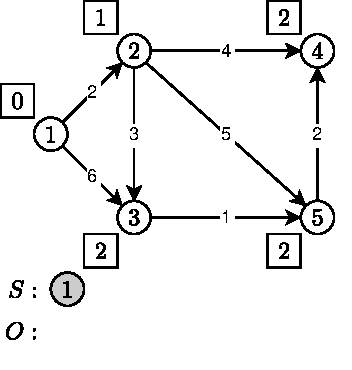
\includegraphics[width=\textwidth]{Chapter_II/KHAN-TOPOLOGICAL-SORT-Example/a.pdf}
		\caption{}
	\end{subfigure}%
	\qquad
	\begin{subfigure}[b]{0.25\textwidth}
		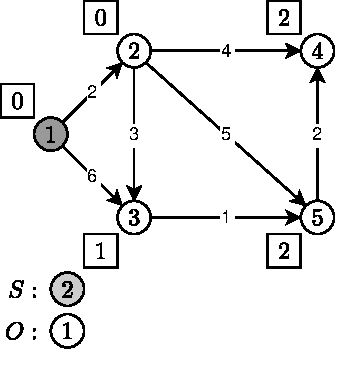
\includegraphics[width=\textwidth]{Chapter_II/KHAN-TOPOLOGICAL-SORT-Example/b.pdf}
		\caption{}
	\end{subfigure}
	\qquad
	\begin{subfigure}[b]{0.25\textwidth}
		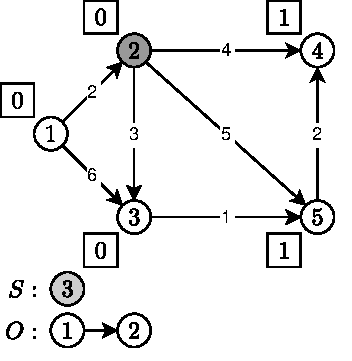
\includegraphics[width=\textwidth]{Chapter_II/KHAN-TOPOLOGICAL-SORT-Example/c.pdf}
		\caption{}
	\end{subfigure}
	\begin{subfigure}[b]{0.25\textwidth}
		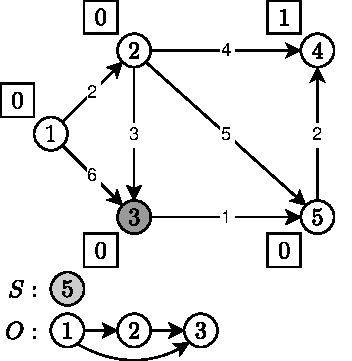
\includegraphics[width=\textwidth]{Chapter_II/KHAN-TOPOLOGICAL-SORT-Example/d.pdf}
		\caption{}
	\end{subfigure}%
	\qquad
	\begin{subfigure}[b]{0.25\textwidth}
		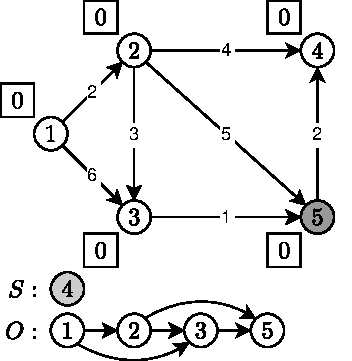
\includegraphics[width=\textwidth]{Chapter_II/KHAN-TOPOLOGICAL-SORT-Example/e.pdf}
		\caption{}
	\end{subfigure}
	\qquad
	\begin{subfigure}[b]{0.25\textwidth}
		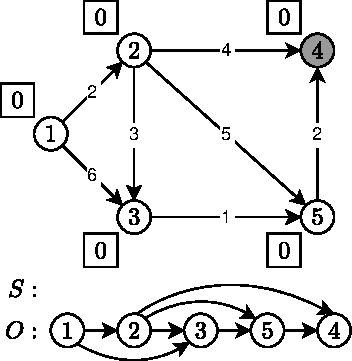
\includegraphics[width=\textwidth]{Chapter_II/KHAN-TOPOLOGICAL-SORT-Example/f.pdf}
		\caption{}
	\end{subfigure}
	\caption{\textbf{Działanie algorytmu Khana} \textbf{(a)} Sytuacja początkowa algorytmu. Na liście $S$ znajdują się wszystkie węzły, do których~--- przed rozpoczęciem działania algorytmu~--- nie wchodziły żadne krawędzie. Przy każdym z~węzłów (w kwadratach) znajduje się liczba takich krawędzi $e \in E$, które wchodzą do danego wierzchołka~--- reprezentują one elementy tablicy $deg \left[ i \right]$, gdzie $i$ to identyfikator węzła, przy którym znajduje się dany element. \textbf{(b)} Algorytm wybiera z~listy $S$ jedyny możliwy element i~usuwa z~grafu wszystkie krawędzie, wychodzące z~wybranego węzła, dodając jednocześnie do listy $O$ każdy węzeł, do którego, w~wyniku usunięcia tych krawędzi, nie prowadzi już żaden łuk. Usuwanie połączenia $v_{i} \overset{1} \leadsto v_{j}$ symbolizujemy zmniejszeniem wartości elementu $deg \left[ j \right]$. \textbf{(c)} Usunięcie krawędzi wychodzących z~następnego, pobranego z~listy $S$ elementu, spowodowało dodanie do niej wierzchołka $v_{3}$. Badany element $v_{2}$~--- podobnie jak w~poprzednim przypadku~--- po wyciągnięciu z~listy $S$, przepinamy do listy $O$. \textbf{(d)} Dodanie do listy $S$ węzła $v_{5}$ w wyniku usunięcia wszystkich krawędzi $e \in \left\{ e_{ij} : i~= 3 \right\}$. Przepięcie badanego elementu $v_{3}$ na listę $O$. \textbf{(e)} Wykonanie kolejnej pętli algorytmu i~dodanie skanowanego elementu $v_{5}$ do listy wynikowej.  \textbf{(f)} Ostatni krok algorytmu. Zauważmy, że w~grafie nie ma już żadnych łuków (wszystkie elementy z~tablicy $deg$ zostały wyzerowane), więc algorytm zakończył się poprawnie~--- badana sieć nie miała cykli.} \label{fig:exampleKhan}
\end{figure}

Czas działania takiej metody jest oczywiście liniowy, zależny od ilości zarówno węzłów, jak i~krawędzi w~grafie. Zależnie od tego, czy w~węzłach przechowujemy informację o~liczbie wchodzących do nich krawędzi, te pierwsze będziemy musieli przejrzeć w~czasie $O \left( \left| V \right| \right)$ w~poszukiwaniu takich węzłów, które takowych krawędzi nie mają, zaś jeżeli takich informacji nie mamy~--- wówczas będziemy musieli je sami wygenerować, skanując wszystkie krawędzie w~grafie (co zajmie nam $O \left( \left| E \right| \right)$ czasu). Bez względu na wcześniej wykonany krok, właściwa część algorytmu polega na usunięciu wszystkich krawędzi z~grafu (gdyż taki chcemy uzyskać rezultat dla prawidłowej sieci) w~czasie $O \left( \left| E \right| \right)$.

\subsection{Przeszukiwanie w~głąb}

Alternatywnym sposobem na topologiczne uporządkowanie grafów w~sieci jest wykorzystanie właściwości, posiadanych przez prosty algorytm przeszukiwania w~głąb, w~skrócie \textsf{DFS} (ang. \textit{Depth-First Search}). Aby posortować topologicznie wszystkie węzły w~gafie $G = \left( V, E \right)$, wykorzystujemy fakt, że wspomniany algorytm oznacza dany węzeł $v$ jako przetworzony dopiero w~momencie, gdy wszystkie węzły, do których jest w~stanie dojść z~badanego węzła, są oznaczone. Innymi słowy nie jest możliwa sytuacja, by w~grafie został oznaczony węzeł, którego wszystkie dzieci (a także jego dalsi potomkowie) nie zostały oznaczone. Zapisując kolejność takich operacji (oznaczania węzłów jako przetworzone) a~następnie odtwarzając ją w~kolejności odwrotnej, uzyskujemy listę z~poprawnie posortowanymi topologicznie węzłami (odwrotna sytuacja do przedstawionej wcześniej ma następującą interpretacje: żaden węzeł $v_{i}$ nie zostanie zaznaczony, gdy istnieje jakikolwiek węzeł $v_{j}$, który jest jeszcze nie zaznaczony, a~który posiada krawędź $v_{j} \overset{1} \leadsto v_{i}$).

\begin{algorithm}[!htbp]
\DontPrintSemicolon
\KwIn{Graf $G = \left( V, E\right)$.}
\KwResult{Lista $O$ z~posortowanymi topologicznie wierzchołkami.}
\Begin{
	Wykonaj \textsf{DFS} dla grafu wejściowego $G$ \;
	Wstaw na początek listy $O$ każdy wierzchołek $v$, kiedy ten tylko zostanie oznaczony jako przetworzony. \;
	\Return $O$ \;
}
\caption{ BFS-TOPOLOGICAL-SORT $\left( G \right)$\label{alg:BFSTopologicalSort}}
\end{algorithm}

W algorytmie niejawnie dokonujemy odwrócenia elementów, które znajdują się na liście $O$, poprzez wstawianie każdego wierzchołka na początek tej listy, nie na jej koniec. Algorytm oczywiście działa w~czasie liniowym, podobnie jak sam \textsf{DFS} ($ \Theta \left( \left| V \right| + \left| E \right| \right)$). Wspomnieliśmy na początku rozdziału, że drugi z~omawianych algorytmów posiada nad pierwszym tę przewagę, że nie przerywa pracy nawet w~momencie napotkania cyklu. Nie jest to do końca prawdą, gdyż zachowanie się algorytmu \textsf{DFS} głównie zależy od intencji jego autora, lecz możemy napisać go w~taki sposób, aby podczas przeglądania grafu wgłąb, po natrafieniu na wierzchołek, który został już odwiedzony, algorytm kontynuował swoją pracę (to jest albo wycofał się z~aktualnie badanego wierzchołka, zaznaczając go jako przetworzony, albo~--- w~przypadku, gdy pozostałe krawędzie badanego węzła prowadzą do jeszcze nieodwiedzonych węzłów~--- kontynuował przeszukiwanie wgłąb). Innymi słowy~--- możemy go zmusić by ignorował cykle, występujące w~badanym grafie.

\begin{figure}[!htbp]
	\centering
	\begin{subfigure}[b]{0.2\textwidth}
		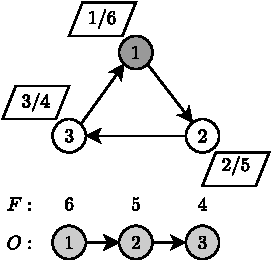
\includegraphics[width=\textwidth]{Chapter_II/BFS-TOPOLOGICAL-SORT-Example/a.pdf}
		\caption{}
	\end{subfigure}%
	\qquad \qquad
	\begin{subfigure}[b]{0.18\textwidth}
		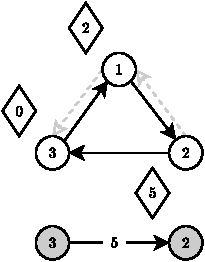
\includegraphics[width=\textwidth]{Chapter_II/BFS-TOPOLOGICAL-SORT-Example/b.pdf}
		\caption{}
	\end{subfigure}
	\qquad \qquad
	\begin{subfigure}[b]{0.18\textwidth}
		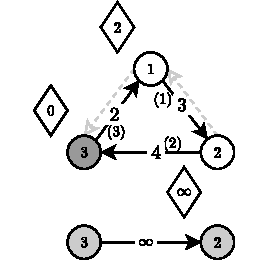
\includegraphics[width=\textwidth]{Chapter_II/BFS-TOPOLOGICAL-SORT-Example/c.pdf}
		\caption{}
	\end{subfigure}
	\caption{\textbf{Przykład złego działania \textsf{DFS} dla grafu z~cyklem} \textbf{(a)} Graf po wykonaniu algorytmu \textsf{DFS}. W~rombach znajdują się charakterystyczne dla grafu wartości w~postaci $x/y$, gdzie $x$ oznacza czas odwiedzenia danego węzła, zaś $y$ to czas jego przetworzenia (po przetworzeniu wszystkich jego dzieci i~ich potomków oraz wycofaniu się z~niego). Lista $O$ zawiera ,,poprawnie'' uporządkowane węzły, w~kolejności malejącej względem czasu przetwarzania węzłów. Algorytm rozpoczyna pracę od pierwszego węzła w~grafie. \textbf{(b)} Poprawnie wykonany algorytm wyszukiwania najkrótszej ścieżki $v_{3} \overset{1} \leadsto v_{2}$~--- $c \left( 3, 2 \right) = \delta \left( 3, 2 \right) = 5$. \textbf{(c)} Błędne rozwiązanie dla algorytmu opartego o~listę $O$ z~rysunku pierwszego. Cyfry w~nawiasach oznaczają kolejność wykonywania relaksacji, wynikającej z~uporządkowania węzłów na liście $O$.} \label{fig:exampleDFS}
\end{figure}

Niestety~---  tak wygenerowany porządek nie nadaje się do wykorzystania w~algorytmie wyszukiwania najkrótszych ścieżek, który działałby w~czasie liniowym. Choć początkowo może się wydawać, że ignorowanie cykli nie szkodzi, a~wręcz jest po naszej myśli (algorytm \textsf{DFS}, napotykając ścieżkę, która zamyka cykl, nie zdecyduje się na pójście tą ścieżką, podobnie jak relaksacja takiej ścieżki nigdy nie przyniesie żadnego rezultatu~--- innymi słowy jest zbędna), lecz prosty przykład wystarcza, by algorytm wyszukiwania najkrótszych ścieżek, który opiera się o~sortowanie topologiczne, zwracał nam niepoprawne wyniki dla tak zadanego grafu.

\subsection{Sortowanie topologiczne}

Jak widzimy z~powyższych przykładów, możliwości wykorzystania sortowania topologicznego w~algorytmach wyszukiwania najkrótszych ścieżek są ograniczone jedynie do małej klasy grafów~--- stanowczo za małej, jeżeli chodzi o~grafy reprezentujące rzeczywiste sieci drogowe. Istnieją jednak pewne problemy (mniej trywialne od pieczenia ciasta, czy kolejności nakładania ubrań), w~których taki algorytm się przydaje i~jest chętnie stosowany głównie ze względu na swoją szybkość działania~--- liniową, proporcjonalnie do ilości krawędzi w~grafie \footnote{Szeregowanie zadań, ustalanie zależności pakietów w systemach operacyjnych, itd.}. Implementacja algorytmu sprowadza się do wykonania relaksacji dla wszystkich krawędzi, wychodzących z~węzłów posortowanych topologicznie, w~której to kolejności powinniśmy postępować.

\begin{algorithm}[!htbp]
\DontPrintSemicolon
\Begin{
	\ForEach{ $v_{i}$ w~porządku topologicznym } {
		\ForEach{$e_{ij} : v_{i} \overset{1} \leadsto v_{j}$}{
			$RELAX \left( v_{i}, v_{j} \right)$ \;
		}
	}
}
\caption{ TOPOLOGICAL-SHORTEST-PATH $\left( G \right)$\label{alg:topologicalShorestPath}}
\end{algorithm}

Aby udowodnić poprawność działania takiego algorytmu, odwołamy się do dwóch wcześniej przedstawionych lematów: o~optymalnej podstrukturze grafu (\ref{lem:optimalSubstructure}) oraz zbieżności najkrótszych ścieżek (\ref{lem:convergenceProperty}).

\begin{proof}
Załóżmy indukcyjnie, że algorytm przeskanował już wierzchołki $v_{i} : i \in \left\{ 1, 2, \cdots, k \right\}$ i~dla każdego z~nich ich waga jest optymalna ($d \left( i \right) = \delta \left( s, v_{i} \right)$). W~oczywisty sposób pierwszy krok indukcyjny jest spełniony: dla $k = 1$ naszym jedynym wierzchołkiem, który został obsłużony, jest wierzchołek początkowy~--- źródło, którego $d \left( s \right) = \delta \left( s, s \right) = 0$. Przyjrzyjmy się teraz sytuacji, w~której algorytm bada węzeł $\left(k+1\right)$'y (nie $v_{k+1}$). Niech najkrótszą ścieżką do tego węzła będzie $P = \left \langle v_{1}, v_{2}, \ldots, v_{h}, k+1 \right \rangle $. Z~lematu \ref{lem:optimalSubstructure} (o optymalnej podstrukturze) wiemy, że każda podścieżka ścieżki $P$ jest najkrótszą ścieżką (w~szczególności jest nią ścieżka $P^{'} = \left \langle v_{1}, v_{2}, \ldots, v_{h} \right \rangle $). Z~faktu, że wszystkie wierzchołki w~grafie są posortowane topologicznie oraz, że krawędź $v_{h} \overset{1}\leadsto k+1 \in E$ (co nam gwarantuje istnienie ścieżki $P$) wynika, że wierzchołek $v_{h}$ jest węzłem, dla którego $h \in \left\{ 1, 2, \cdots, k \right\}$~--- w~związku z~tym, na mocy założenia indukcyjnego, wartość $v_{h}.d = \delta \left( s, v_{h} \right)$. Zgodnie z~lematem \ref{lem:convergenceProperty}, jeżeli w~dowolnym momencie przed relaksacją krawędzi $v_{h} \overset{1}\leadsto k+1$ wartość $v_{h}.d = \delta \left( s, v_{h} \right)$, to po relaksacji tej krawędzi już zawsze $ \left( k+1 \right).d = \delta \left( s, k+1 \right) $ (jest optymalna). Z~faktu istnienia takiej krawędzi oraz z~uporządkowania topologicznego wszystkich węzłów w~grafie wiemy, że waga, jaką posiada wierzchołek $v_{h}$, zawsze będzie optymalna przed przystąpieniem do przechodzenia po krawędzi $v_{h} \overset{1}\leadsto k+1$, co kończy dowód.
\end{proof}


\begin{figure}[!htbp]
	\centering
	\begin{subfigure}[b]{0.18\textwidth}
		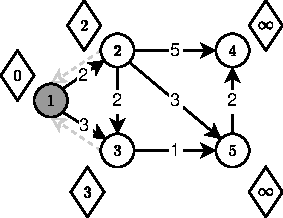
\includegraphics[width=\textwidth]{Chapter_II/TOPOLOGIC-SHORTEST-PATH-Example/a.pdf}
		\caption{}
	\end{subfigure}
	\begin{subfigure}[b]{0.18\textwidth}
		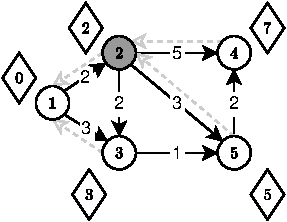
\includegraphics[width=\textwidth]{Chapter_II/TOPOLOGIC-SHORTEST-PATH-Example/b.pdf}
		\caption{}
	\end{subfigure}
	\begin{subfigure}[b]{0.18\textwidth}
		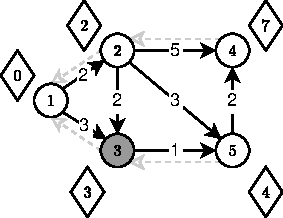
\includegraphics[width=\textwidth]{Chapter_II/TOPOLOGIC-SHORTEST-PATH-Example/c.pdf}
		\caption{}
	\end{subfigure}
	\begin{subfigure}[b]{0.18\textwidth}
		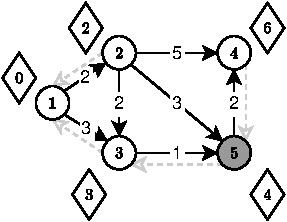
\includegraphics[width=\textwidth]{Chapter_II/TOPOLOGIC-SHORTEST-PATH-Example/d.pdf}
		\caption{}
	\end{subfigure}
	\begin{subfigure}[b]{0.18\textwidth}
		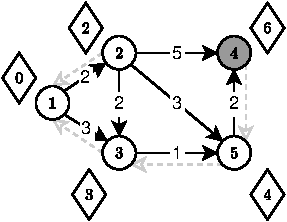
\includegraphics[width=\textwidth]{Chapter_II/TOPOLOGIC-SHORTEST-PATH-Example/e.pdf}
		\caption{}
	\end{subfigure}
	\caption{\textbf{Przykład dla ustalonego porządku topologicznego węzłów: $v_{1}, v_{2}, v_{3}, v_{5}, v_{4}$.}} \label{fig:exampleTopologicalShotrestPath}
\end{figure}

\newpage
\section{Generyczny algorytm Dijkstry}
\label{sec:dijkstraGenericAlgorithm}

Pokazaliśmy w~poprzednich rozdziałach, że kolejność przetwarzania węzłów może mieć ogromny wpływ na szybkość działania algorytmu~--- od przeglądania wierzchołków w~kolejności narzuconej nam przez ich uporządkowanie w~strukturach grafu (w czasie $ O \left( \left| V \right| \cdot \left| E \right| \right)$), aż do badania wierzchołków w~porządku topologicznym ($ O \left( \left| V \right| + \left| E \right| \right)$). Oba te algorytmy miały zasadnicze wady: albo działały w~czasie dużo poniżej naszych oczekiwań, wykonując zatrważającą ilość niepotrzebnych operacji, albo nie nadawały się do użytku w~sieciach, które my chcemy badać (z nieujemnymi cyklami). W~tym rozdziale przedstawimy kolejny sposób przeglądania wierzchołków grafu $G = \left( V, E \right)$, pokażemy generyczny algorytm na nim opartym, a~także udowodnimy jego poprawność. Bazując na kontrprzykładzie, wykażemy także, że nie działa on dla grafów, które zawierają krawędzie o~ujemnych wagach (a co za tym idzie~--- dla grafów z~ujemnymi cyklami). Algorytm, opracowany przez holenderskiego informatyka Edsgera Dijkstrę, okaże się podstawą do powstania szeregu jego modyfikacji, którym niejednokrotnie zawdzięcza asymptotycznie szybsze czasy działania, a~które omówimy w~tym rozdziale, skupiając się na ich własnościach.

\subsection{Algorytm Dijkstry}
\label{sub:dijkstraAlgorithm}

Sama idea algorytmu jest bardzo podobna do poprzedniej tj. zakłada wykonywanie relaksacji dla wszystkich krawędzi aktualnie badanych wierzchołków, których to kolejność jest w~specyficzny sposób ustalana. W~Przypadku algorytmu Dijkstry mamy regułę, która mówi, że wierzchołki są skanowane w~niemalejącej kolejności ich etykiet (atrybutów $d$~--- odległości węzła od źródła $s$), co wiąże się z~wykorzystaniem w~naszym algorytmie \textbf{kolejek priorytetowych}, które zapewniają nam właśnie taki porządek. Jak się później okaże~--- omawiane modyfikacje algorytmu Dijkstry różnią się głównie jej implementacją~\cite[$4.5$]{Ahuja:1993:NFT:137406}.

Przyjmiemy, że mamy dwa zbiory rozłączne: $S$, który na początku działania algorytmu jest pusty~--- do niego trafiać będą przetworzone już wierzchołki~--- oraz $\overline{S}$, w~którym na początku przechowywane są wszystkie węzły. Jak już wspomnieliśmy, algorytm ma za zadanie sekwencyjne pobierać ze zbioru $\overline{S}$ takie wierzchołki $v_{i}$, by $v_{i}.d = \min \left\{ v_{j}.d : v_{j} \in \overline{S} \right\}$, przenosić je do zbioru wierzchołków $S$ oraz wykonywać relaksacje dla każdej krawędzi, która wychodzi z~tego wierzchołka. Oczywiście~--- tak jak w~każdym poprzednim algorytmie~--- na początku inicjalizujemy graf metodą \textsc{INIT-GRAPH} $\left( G, s \right)$. Pseudokod generycznego algorytmu Dijkstry wygląda tak, jak przedstawiono poniżej.

\begin{algorithm}[!htbp]
\DontPrintSemicolon
\Begin{
	$S \longleftarrow \emptyset $ \;
	$\overline{S} \longleftarrow \left\{ v : v \in V \right\} $ \;
	\While{$\overline{S}$ nie jest pusty} {
		$v \longleftarrow  v_{i} : v_{i}.d = \min \left\{ v_{j}.d : v_{j} \in \overline{S} \right\}$ \;
		$S \longleftarrow S \cup \left\{ v \right\}$ \;
		$\overline{S} \longleftarrow \overline{S} - \left\{ v \right\}$ \;
		\ForEach{$e_{ij} : v_{i} \overset{1} \leadsto v_{j}$}{
			$RELAX \left( v_{i}, v_{j} \right)$ \;
		}
	}
}
\caption{ GENERIC-DIJKSTRA $\left( G, s \right)$\label{alg:GenericDijksta}}
\end{algorithm}

W faktycznej implementacji linijki $5$--$7$ zwykle zastępuje się operacją $\textrm{\textsc{EXTRACT-MIN}} \left( Q \right)$, gdzie $Q$ to nasza kolejka priorytetowa. Zbioru $S$ zaś w~ogóle się nie uwzględnia, gdyż służy on tylko do celów przeprowadzenia dowodów poprawności tego algorytmu i~wykazania, że jest on poprawnie skonstruowany (niezmiennikiem pętli $4$--$9$ w~tym przypadku będzie $Q = V - S$). Odnajdywaniem najmniejszego elementu (w sensie dystansu wierzchołka do źródła) i~usuwaniem go ze zbioru $\overline{S}$ zajmuje się, wymieniona wyżej, operacja (wtedy $\overline{S} = Q$). Na przykładzie \ref{fig:exapleDijkstraDLList} jako kolejkę priorytetową wykorzystano podwójnie wiązaną listę (która oczywiście nie jest najfortunniejszym wyborem), której czas potrzebny na wyciągnięcie z~niej najmniejszego elementu, jest zależny od ilości tych elementów na liście (w najgorszym przypadku $ \left| V \right| $).

\begin{figure}[!h]
	\centering
	\begin{subfigure}[b]{0.3\textwidth}
		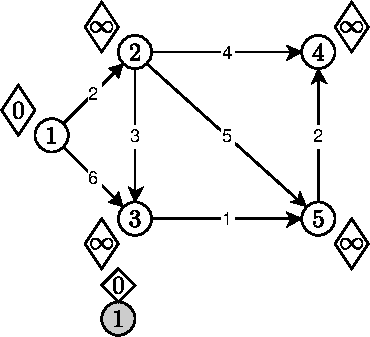
\includegraphics[width=\textwidth]{Chapter_II/DIJKSTRA-DLList/a.pdf}
		\caption{}
	\end{subfigure}%
	\begin{subfigure}[b]{0.3\textwidth}
		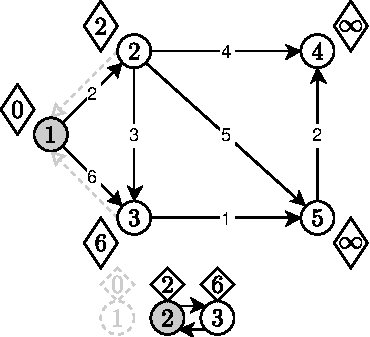
\includegraphics[width=\textwidth]{Chapter_II/DIJKSTRA-DLList/b.pdf}
		\caption{}
	\end{subfigure}
	\begin{subfigure}[b]{0.3\textwidth}
		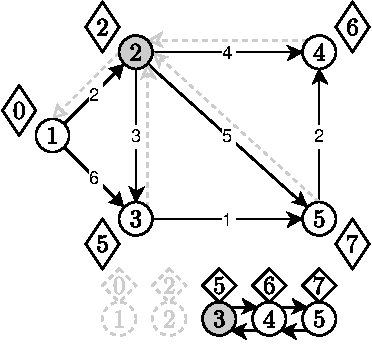
\includegraphics[width=\textwidth]{Chapter_II/DIJKSTRA-DLList/c.pdf}
		\caption{}
	\end{subfigure}
	\begin{subfigure}[b]{0.3\textwidth}
		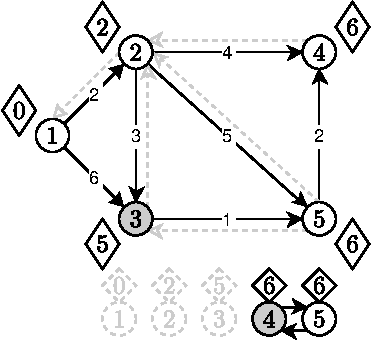
\includegraphics[width=\textwidth]{Chapter_II/DIJKSTRA-DLList/d.pdf}
		\caption{}
	\end{subfigure}%
	\begin{subfigure}[b]{0.3\textwidth}
		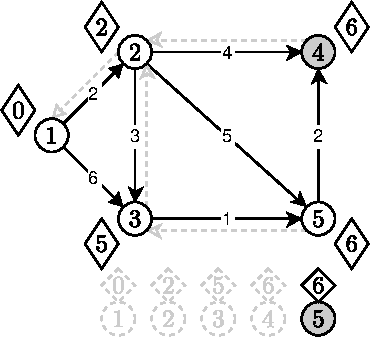
\includegraphics[width=\textwidth]{Chapter_II/DIJKSTRA-DLList/e.pdf}
		\caption{}
	\end{subfigure}
	\begin{subfigure}[b]{0.3\textwidth}
		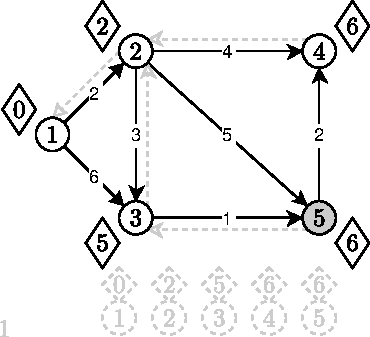
\includegraphics[width=\textwidth]{Chapter_II/DIJKSTRA-DLList/f.pdf}
		\caption{}
	\end{subfigure}
	\caption{\textbf{Działanie algorytmu Dijkstry} \textbf{(a)} Sytuacja po zainicjowaniu grafu $G = \left( V, E \right)$ przez \textsf{INIT-GRAH} ze źródłem $v_{s}.id = 1$. \textbf{(b)} Z~listy dwukierunkowej został wyciągnięty najmniejszy element i~została wykonana operacja \textsc{RELAX} dla krawędzi: $e_{12}$ i~$e_{13}$. Odpowiednio węzły $v_{2}$ i~$v_{3}$ zostały wstawione do kolejki. \textbf{(c)} Najmniejszym elementem na liście był węzeł $v_{2}$. Został usunięty z~kolejki, algorytm wykonał relaksację krawędzi $e_{23}$, $e_{24}$ i~$e_{25}$. Etykieta węzła $v_{3}$ uległa zmniejszeniu. \textbf{(d--f)} Kroki analogiczne jak poprzednie.} \label{fig:exapleDijkstraDLList}
\end{figure}

\subsection{Złożoność obliczeniowa}

Analizując złożoność czasową algorytmu, widzimy że jego główna pętla $4$--$9$ wykonuje się dokładnie $ \left| V \right| $ razy, za każdym razem usuwając z~kolejki priorytetowej dokładnie jeden węzeł, gdzie skanowane węzły nie powtarzają się \footnote{Ilość wykonywanych pętli możemy ograniczyć, kończąc algorytm, gdy z~kolejki zostanie wyjęty taki węzeł $v$, że $v.d = \infty$. Jak wiemy, relaksacja żadnej krawędzi wychodzącej z~takiego węzła nie zmieni nam sytuacji w~grafie, a~z własności kolejki priorytetowej wiemy, że pozostałe elementy $u$ , które w~niej zostały, spełniają $u.d \geqslant v.d = \infty$.}. Następnie, wewnątrz pętli, wyszukiwany jest najmniejszy element w~kolejce~--- czas tej operacji jest naturalnie zależny od wybranego przez nas sposobu jej implementacji i~--- na pożytek naszych rozważań~--- niech zajmuje czas $O \left( \textrm{\textsc{EXTRACT-MIN}} \left( Q \right) \right)$. Takich operacji podczas działania algorytmu wykonamy $ \left| V \right| $. Dla każdego węzła, wyjętego z~kolejki, dla wszystkich łuków, wychodzących z~danych węzłów, wykonywana jest operacja relaksacji~--- łatwo zauważyć, że podczas całej procedury metoda \textsc{RELAX} zostanie wywołana dokładnie $ \left| E \right|$ razy, podczas której może być wymagane zmniejszenie atrybutu $d$ któregoś z~węzłów~--- koszt takiej operacji jest znowu zależny od implementacji kolejki priorytetowej (wraz ze zmniejszeniem się klucza może zajść konieczność przemieszczenia węzła bliżej głowy kolejki) i~dla naszej analizy niech wyniesie $O \left( \textrm{\textsc{DECREASE-KEY}} \left( Q, v, k \right) \right)$, gdzie $k$ to nowy klucz (nowa odległość od źródła $s$~--- $v.d$) węzła $v$. Pozostaje nam jeszcze metoda $\textrm{\textsc{INSERT}} \left( Q, v \right)$, która wstawia nam elementy do kolejki. Czas jej działania jest również zależny od wybranej implementacji kolejki $Q$, zaś miejsce jej wywołania zależne jest już od woli programisty; może on przed rozpoczęciem algorytmu wstawić wszystkie wierzchołki grafu do kolejki (wiersz $3$), bądź też wstawiać je na bieżąco w~chwili, gdy algorytm potrafi już do nich dojść (wtedy podczas relaksacji podejmowana jest decyzja czy wstawić nowy element do kolejki, czy taki już w~kolejce istnieje i~należy tylko zmniejszyć jego klucz oraz~zadbać o~zachowanie prawidłowego porządku w~strukturze danych). Bez względu na preferowane rozwiązanie ilość takich operacji wyniesie dokładnie $ \left| V\right|$, jako że każdy wierzchołek wstawimy do kolejki (i wyjmiemy go z~niej) tylko raz. Reasumując~--- złożoność algorytmu Dijkstry w~uogólnionym przypadku jest ograniczona z~góry przez:

\begin{equation}
O \left( \left| E \right| \cdot O \left( \textrm{\textsc{DECREASE-KEY}} \left( Q, v, k \right) \right) + \left| V \right| \cdot \left[ O \left( \textrm{\textsc{INSERT}} \left( Q, v \right) \right) + O \left( \textrm{\textsc{EXTRACT-MIN}} \left( Q \right) \right) \right] \right)
\end{equation}\label{eq:dijkstraComplexity}.

\textbf{Wąskim gardłem} algorytmu nazywamy taki jego element składowy, który przesądza o~złożoności obliczeniowej całego algorytmu, niejednokrotnie go zwalniając. W~tym przypadku nie ma wątpliwości, że takim elementem w~algorytmie Dijkstry jest zastosowana struktura, odpowiedzialna za wykonywanie tych trzech operacji.

\subsection{Ujemne koszty krawędzi}

Nim udowodnimy poprawność algorytmu Dijkstry, przeanalizujemy jeszcze prosty przykład, w~którym dopuścimy wystąpienie krawędzi o~ujemnym koszcie i~pokażemy, że dla takiego grafu nasz algorytm zwróci błędny wynik.

\begin{figure}[!htbp]
	\centering
	\begin{subfigure}[b]{0.3\textwidth}
		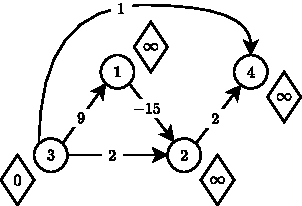
\includegraphics[width=\textwidth]{Chapter_II/DIJKSTRA-NegativeArc/a.pdf}
		\caption{}
	\end{subfigure}%
	\begin{subfigure}[b]{0.3\textwidth}
		\includegraphics[width=\textwidth]{Chapter_II/DIJKSTRA-NegativeArc/b.pdf}
		\caption{}
	\end{subfigure}
	\begin{subfigure}[b]{0.3\textwidth}
		\includegraphics[width=\textwidth]{Chapter_II/DIJKSTRA-NegativeArc/c.pdf}
		\caption{}
	\end{subfigure}
	\begin{subfigure}[b]{0.3\textwidth}
		\includegraphics[width=\textwidth]{Chapter_II/DIJKSTRA-NegativeArc/d.pdf}
		\caption{}
	\end{subfigure}%
	\begin{subfigure}[b]{0.3\textwidth}
		\includegraphics[width=\textwidth]{Chapter_II/DIJKSTRA-NegativeArc/e.pdf}
		\caption{}
	\end{subfigure}
	\caption{\textbf{Działanie algorytmu Dijkstry w~grafie z~ujemnymi kosztami krawędzi}} \label{fig:exapleDijkstraNegativArc}
\end{figure}

Jak powiedzieliśmy, algorytm Dijkstry analizuje wierzchołki grafu $G = \left( V, E \right)$ w~ściśle określonym porządku tj. bada zawsze taki węzeł $v$ , którego $v.d$ jest najmniejsze spośród wszystkich pozostałych, jeszcze nie przeanalizowanych węzłów. Na kolejnych rysunkach zaznaczono kolejność przeglądania węzłów jaka wynika z~tej własności (za węzeł startowy przyjęliśmy $v_{3}$). Widzimy, że algorytm zwrócił błędną ścieżkę dla pary węzłów: $v_{3}$ i~$v_{4}$ (poprawną, najkrótszą ścieżką $v_{3} \overset{*}\leadsto v_{4}$ jest ścieżka $ P = \left \langle v_{3}, v_{1}, v_{2}, v_{4} \right \rangle $ o koszcie $-4$, nie zaś ścieżka $ P^{'} = \left \langle v_{3}, v_{4} \right \rangle $ ) ze względu na wystąpienie w~grafie krawędzi o~ujemnym koszcie. Problemem tutaj jest oczywiście niepoprawna kolejność, w jakiej algorytm otrzymywał informację o wierzchołkach (koszt dotarcia do węzła $v_{2}$ okazuje się w rzeczywistości dużo mniejszy dopiero, gdy algorytm wykona relaksacje dla krawędzi wychodzących z wierzchołka $v_{1}$, który ma najniższy priorytet).
\newpage

\subsection{Poporawność działania}

\begin{figure}[!htbp]
	\includegraphics[width=0.3\textwidth]{Chapter_II/ProofOfDijkstra/a.pdf}
	\caption{\textbf{Dowód poprawności algorytmu Dijkstry}} Tuż przed wstawieniem wierzchołka $v_{j}$ do $S$ ten ostatni nie jest pusty. Przerywanymi strzałkami zaznaczono ścieżki $p_{1}$ oraz $p_{2}$, które mogą mieć dowolnie dużą ilość składowych (w skrajnym przypadku $s = x$ i/lub $y = v_{j}$). Dodatkowo $x \neq y$. \label{fig:proofOfDijkstra}
\end{figure}

\begin{proof}
\label{pr:dijkstra}
Załóżmy indukcyjnie, że dla każdego węzła $v_{i}$ w~momencie dodawania go do zbioru wierzchołków przetworzonych $S$ zachodzi $v_{i}.d = \delta \left( s, v_{i} \right)$. Pierwszy krok indukcyjny jest oczywisty, gdyż na samym początku zbiór $S$ jest pusty i~założenie jest prawdziwe. Pierwszym wierzchołkiem, który jest dodawany do tego zbioru, jest wierzchołek $s$ będący źródłem, którego w~oczywisty sposób $s.d = 0 = \delta \left( s, s \right)$ (w grafie dla algorytmu Dijkstry założyliśmy brak krawędzi o~ujemnych długościach). Przyjmijmy nie w~prost, że istnieje w~grafie taki wierzchołek $v_{j}$, dla którego $v_{j}.d \neq \delta \left( s, v_{j} \right)$ w~trakcie jego dodawania do zbioru $S$ i~będzie on pierwszym takim wierzchołkiem, jaki będziemy chcieli do tego zbioru dodać. Wiemy, że $v_{j} \neq s$ oraz, że do takiego wierzchołka na pewno istnieje najkrótsza ścieżka ze źródła $s$ (gdyby tak nie było to odpowiednio wtedy $v_{j}.d = s.d = 0 = \delta \left( s, s \right) = \delta \left( s, v_{j} \right)$ lub $v_{j}.d = \delta \left( s, v_{j} \right) = \infty $~--- z~własności braku ścieżki). Bezpośrednio z~poprzednich spostrzeżeń wynika, że w~momencie dodawania wierzchołka $v_{j}$ do zbioru $S$ ten jest niepusty i~zawiera co najmniej jeden element~--- źródło. Niech istniejąca ścieżka z~$s$ do $v_{j}$ nazywa się $P$. Rozważmy sytuację taką, jaką widać na rysunku \ref{fig:proofOfDijkstra}. Rozbiliśmy na nim ścieżkę $P$ na dwie składowe: $p_{1}$ i~$p_{2}$, gdzie $v_{s} \overset{p_{1}}\leadsto x \overset{1}\leadsto y \overset{p_{2}}\leadsto v_{j}$ oraz pierwsza z~nich składa się tylko z~węzłów należących do zbioru $S$, zaś druga~--- tylko z~węzłów poz tym zbiorem. Dodatkowo, węzeł $y$ jest pierwszym na ścieżce $P$, który jest poza tym zbiorem. Pokażemy teraz, że w~momencie dodawania wierzchołka $v_{j}$ ($v_{j}.d \neq \delta \left( s, v_{j} \right)$) do zbioru $S$ zachodzi $y.d = \delta \left( s, y \right)$. Aby udowodnić ten fakt, wystarczy zauważyć, że skoro wierzchołek $v_{j}$ był pierwszym takim, dla którego zachodzi $v_{j}.d \neq \delta \left( s, v_{j} \right)$, to wstawiając do zbioru $S$ wierzchołek $x$ na pewno $v_x.d = \delta \left( s, x \right)$, a~ze zbieżności (lemat \ref{lem:convergenceProperty}) mamy, że zachodzi również $y.d = \delta \left( s, y \right)$ (w trakcie dodawania wierzchołka $x$ do zbioru $S$ zajdzie relaksacja krawędzi $x \overset{1}\leadsto y$, gdzie wcześniej $v_x.d = \delta \left( s, x \right)$).

Ponieważ na naszym rysunku wierzchołek $y$ występuje na ścieżce $P$ wcześniej od wierzchołka $v_{j}$ i~każda krawędź w~grafie ma koszt nieujemny, to $ \delta \left( s, y \right) \leqslant \delta \left( s, v_{j} \right) $. Z tego wnioskujemy, że:

\begin{equation}
\begin{aligned}
y.d &= \delta \left( s, y \right) \\
&\leqslant \delta \left( s, v_{j} \right) \\
&\leqslant v_{j}.d \; \; \textrm{(z lematu \ref{lem:costUpperBound} o~górnym ograniczeniu)}
\end{aligned}
\end{equation}

Wiemy jednak, że z~własności algorytmu Dijkstry zawsze wybieramy wierzchołek spoza zbioru $S$ o~jak najmniejszej wartości atrybutu $d$~--- skoro oba wierzchołki ($y$ i~$v_{j}$) nie należą do zbioru $S$ w~chwili wyboru wierzchołka $v_{j}$, mamy zagwarantowane, że $v_{j}.d = \min \left\{ v.d : v \notin S \right\}$ (w~szczególności $v_{j}.d \leqslant y.d$). Dodając to ostatnie równanie do szeregu poprzednich nierówności otrzymujemy:

\begin{equation}
y.d = \delta \left( s, y \right) = \delta \left( s, v_{j} \right) = v_{j}.d
\end{equation}

Widzimy, że $ v_{j}.d = \delta \left( s, v_{j} \right) $, co jest sprzeczne z~naszym założeniem (dodanie do zbioru $S$ pierwszego wierzchołka $v_{j}$ o~własności  $v_{j}.d = \delta \left( s, v_{j} \right) $). Rozumowanie jest identyczne w~przypadku, gdyby na ścieżkach $p_{1}$ i/lub $p_{2}$ znajdowała się dowolna liczba węzłów, spełniających nasze założenia. Pokazaliśmy zatem, że dla każdego wierzchołka $v \in V$, w~momencie jego dodawania do zbioru $S$, zachodzi $v.d = \delta \left( s, v \right)$. Algorytm kończy działanie, gdy w~kolejce $Q$ nie ma już żadnych wierzchołków (wszystkie zostały dodane do zbioru $S$), tak więc w~momencie, gdy każdy wierzchołek spełnia $v.d = \delta \left( s, v \right)$, co kończy dowód.
\end{proof}

\section{Podstawowe struktury danych}

Jak pokazaliśmy wcześniej~--- efektywność algorytmu Dijkstry w~głównej mierze zależy od efektywności implementacji struktury, od której będziemy wymagać wykonywania trzech, podstawowych operacji: $\textrm{\textsc{INSERT}} \left( Q, v \right)$, $\textrm{\textsc{EXTRACT-MIN}} \left( Q \right)$ i~$\textrm{\textsc{DECREASE-KEY}} \left( Q, v, k \right)$. Wyspecjalizowanymi strukturami do ich wykonywania są kolejki priorytetowe, choć~--- jak mogliśmy się już przekonać~--- inne struktury, takie jak tablice, listy jednokierunkowe czy podwójnie wiązane (ang. \textit{double-linked lists}), także umożliwiają nam poprawną konstrukcję algorytmu Dijkstry. Korzystając z~nich, musimy jednak płacić cenę za ich wysoką nieefektywność (dla listy dwukierunkowej, wykorzystanej przy omawianiu algorytmu, wyszukanie najmniejszego elementu kosztuje nas proporcjonalnie do ilości wierzchołków, znajdujących się na niej w~trakcie wyszukiwania). Jeżeli spojrzymy na złożoność algorytmu Dijkstry (\ref{eq:dijkstraComplexity}), natychmiastowo uzyskamy górne ograniczenie na poziomie $ O \left( \left| V \right| ^{2} \right)$, co niewiele oddala nas złożoności tak prostego algorytmu, jakim jest algorytm Bellmana-Fora.


Mówiąc o~różnych wcieleniach algorytmu Dijkstry, nie sposób jest więc nie poruszyć tematu podstawowych struktur danych, jakie możemy wykorzystać do implementacji różnych kolejek priorytetowych, ich właściwości i~czasu działania podstawowych operacji, których wykonywanie dane struktury umożliwiają~--- w~szczególności $\textrm{\textsc{INSERT}} \left( Q, v \right)$, $\textrm{\textsc{EXTRACT-MIN}} \left( Q \right)$ i~$\textrm{\textsc{DECREASE-KEY}} \left( Q, v, k \right)$. W~niniejszym rozdziale omówimy takie struktury jak: kopce binarne (w uogólnionym spojrzeniu na kopce $R$-arne), kopce Fibonacciego, kolejki z~przepełnieniem oraz szereg innych pomysłów, opartych o~kontenery, zwane dalej kubełkami (ang. \textit{buckets}).

\section{Struktury oparte na kopcach}

Jedną ze struktur, przystosowanych do operacji charakterystycznych dla kolejki priorytetowej, jest kopiec (ang. \textit{heap}). Jego najogólniejszą własnością jest to, że operacja, zwracająca najmniejszy (lub największy) element, który znajduje się w~kopcu, działa w~czasie stałym i~polega na odwołaniu się do szczytu takiego kopca. Kopce to szczególne przypadki drzew, gdzie pomiędzy rodzicem a~potomkami zwykle jest ustalona stała relacja (w przypadku, który nas interesuje, klucze przechowywane przez potomków węzła $v$ powinny być zawsze większe od klucza rodzica: $v.d \leqslant v_{i} : v_{i}.\Pi = v$~--- właściwość kopca typu \textsc{min}). Przedstawimy dwa, powszechnie znane rodzaje kopców: zwykły, do którego implementacji wykorzystamy tablicę, rozszerzając powszechną implementację jego binarnej wersji, oraz kopiec Fibonacciego, który~--- jak się okaże~--- pomimo swojej teoretycznej przewagi w~szybkości wykonywania poszczególnych operacji, w~praktyce często działa wolniej od wspomnianej wcześniej wersji, znacznie prostszej w implementacji.

\subsection{Kopiec R-arny}

Kopien $R$-arny jest uogólnieniem kopca binarnego~--- podczas gdy dla tego drugiego każdy rodzic może posiadać do $2$ potomków, w~pierwszym przypadku takich węzłów rodzic może mieć od $0$ do $R$, co zauważalnie zmniejsza wysokość takiego kopca (kosztem jego szerokości). Poniższa tabelka przedstawia koszty poszczególnych operacji dla kopca binarnego i~$R$-arnego:

\begin{center}
	\begin{tabular}{ccc}
		& \multicolumn{2}{c}{Kopiec} \\
		\cline{2-3}
		Operacja & binarny & $R$-arny \\
		\hline
		$\textrm{\textsc{INSERT}} \left( Q, v \right)$ & $O \left( \log \left( n \right) \right)$ & $O \left( \log_{R} \left( n \right) \right)$ \\
		$\textrm{\textsc{EXTRACT-MIN}} \left( Q \right)$ & $O \left( \log \left( n \right) \right)$ & $O \left( R \cdot \log_{R} \left( n \right) \right)$ \\
		$\textrm{\textsc{DECREASE-KEY}} \left( Q, v, k \right)$ & $O \left( \log \left( n \right) \right)$ & $O \left( \log_{R} \left( n \right) \right)$  \\
		\hline
	\end{tabular}
\end{center}

\subsubsection{Implementacja}

Algorytm wyszukiwania najkrótszych ścieżek oparty na strukturze $D$-arnego kopca jest jedynym algorytmem, który nie wymaga od nas tworzenia dodatkowych struktur. Jak dobrze wiemy, jedną z~właściwości kopców jest ich zdolność do pracy w~miejscu tj. nie wykorzystywania dodatkowej pamięci podczas działania. Pod pojęciem naszego grafu $G = \left( V, E \right)$ kryje się tablica $tab \left[ 1 \cdots \left| V\right| \right]$, przechowująca wierzchołki indeksowane ich identyfikatorami ($tab[i]=v_{i}$), oraz listy sąsiedztwa, które są przyporządkowane do każdego z~takich węzłów. Aby skorzystać z~właściwości kopca, będziemy chcieli zbudować jego strukturę bezpośrednio na wspomnianej tablicy węzłów tj. kopiec o~$k$ elementach będziemy chcieli przedstawić jako tablica $vertices \left[ 1 \cdots k \right]$. W~takiej sytuacji, jeżeli dowolny wierzchołek $v$ znajduje się na pozycji $i <= k $ w~tablicy $tab$, to znaczy, że w~którymś momencie został on wstawiony do naszej kolejki priorytetowej i~nie opuści jej, dopóki nie stanie się on najmniejszy spośród tych $k$ elementów. Aby jednak nie stracić informacji o~pierwotnym rozmieszczeniu wierzchołków w~tablicy $tab$, będziemy chcieli wprowadzić pomocniczą tablicę $heapIDArray \left[ 1 \cdots \left| V\right| \right]$, której to wartości będą odzwierciedlać faktyczne rozmieszczenie wierzchołków w~$tab$ po modyfikacjach ($tab \left[ heapIDArray \left[ i \right] \right] = v_{i}$), jakich dopuści się na niej nasza kolejka priorytetowa (indeksami tablicy $tab$ pierwotnie były identyfikatory wierzchołków, a~ich nie możemy zmieniać).

Zasada działania takiego kopca nie różni się niczym od zastosowania takiej samej struktury do posortowania $n$ liczb, gdzie rozmiar kopca monotonicznie rośnie w~trakcie jego budowania a~następnie maleje w~czasie działania takiego algorytmu. W~naszym przypadku liczba jego elementów może się zwiększać jak i~zmniejszać w~dowolnej kolejności~--- jeżeli się zwiększa, to ostatni element w~części tablicy należącej do powiększonego kopca zamieniamy z~elementem, który chcemy faktycznie do niego wstawić, następnie ,,wypychając'' go ku górze (analogiczna procedura jest wykonywana podczas powiększania kopca w~czasie jego budowania dla algorytmu sortowania). W przypadku odwrotnym (jeżeli rozmiar kopca maleje)~--- zachowanie, w~porównaniu z~algorytmem sortującym, jest identyczne.

\begin{figure}[!htbp]
	\centering
	\begin{subfigure}[b]{0.33\textwidth}
		\includegraphics[width=\textwidth]{Chapter_II/R-HEAP-Example/a.pdf}
		\caption{}
	\end{subfigure}%
	\begin{subfigure}[b]{0.33\textwidth}
		\includegraphics[width=\textwidth]{Chapter_II/R-HEAP-Example/b.pdf}
		\caption{}
	\end{subfigure}
	\begin{subfigure}[b]{0.33\textwidth}
		\includegraphics[width=\textwidth]{Chapter_II/R-HEAP-Example/c.pdf}
		\caption{}
	\end{subfigure}
	\begin{subfigure}[b]{0.33\textwidth}
		\includegraphics[width=\textwidth]{Chapter_II/R-HEAP-Example/d.pdf}
		\caption{}
	\end{subfigure}%
	\begin{subfigure}[b]{0.33\textwidth}
		\includegraphics[width=\textwidth]{Chapter_II/R-HEAP-Example/e.pdf}
		\caption{}
	\end{subfigure}
	\begin{subfigure}[b]{0.33\textwidth}
		\includegraphics[width=\textwidth]{Chapter_II/R-HEAP-Example/f.pdf}
		\caption{}
	\end{subfigure}
	\caption{\textbf{Działanie algorytmu Dijkstry w~oparciu o~kopiec $R$-arny} \textbf{(a)} Sytuacja po zainicjowaniu grafu $G$ przez \textsf{INIT-GRAH} ze źródłem $v_{1}$. W~tablicy na szaro zaznaczone są elementy należące do kopca, przedstawionego poniżej. Niech $k$ oznacza rozmiar kopca, tablica $tab$ jest indeksowana od $1$. \textbf{(b)} Z~kopca zostaje usunięty węzeł $v_{1}$ ($k=0$). W~wyniku relaksacji na kopiec zostaje przeniesiony węzeł $v_{2}$ ($k=1$ i~$tab \left[ k \right] = v_{2}$), zaś na stare miejsce wstawionego węzła zostaje przeniesiony węzeł $v_{1}$. Analogicznie na koniec kopca wstawiany jest $v_{3}$  ($k=2$, $tab \left[ k \right] = v_{3}$), w~wyniku czego $tab \left[ 3 \right] = v_{1}$. \textbf{(c)} Z~kopca zostaje pobrany węzeł $v_{2}$ a~na szczyt stosu zostaje przeniesiony ostatni element w~kopcu ($v_{3}$). W~wyniku relaksacji krawędzi wychodzących z~pobranego węzła do kopca zostają dodane węzły: $v_{4}$ i~$v_{5}$. Tablica $tab$ zmienia się odpowiednio: $\left\{ 3 \right\} \left[ 2 \right]  \left[ 1 \right]  \left[ 4 \right]  \left[ 5 \right] \rightarrow \left\{ 3 \right\} \left\{ 4 \right\}  \left[ 1 \right]  \left[ 2 \right]  \left[ 5 \right] \rightarrow \left\{ 3 \right\} \left\{ 4 \right\}  \left\{ 5 \right\}  \left[ 2 \right]  \left[ 1 \right]$, gdzie w~klamrach ,,$\left\{\right\}$''~ zostały zaznaczone węzły znajdujące się w~kopcu. Żadna operacja nie narusza własności kopca. \textbf{(d)} Wybrano kolejny węzeł ze szczytu stosu: $v_{3}$, zamieniono go z~ostatnim elementem w~kopcu i~zmniejszono jego rozmiar ($k=2$). Zachowana jest własność kopca. W~wyniku relaksacji zostają zmienione atrybuty: $v_{5}.\Pi = v_{3}$ i~$v_{5}.d = 4$. \textbf{(e--f)} Z~kopca zostaje zabrany jego najmniejszy element: $v_{5}$ i~wykonywana jest operacja \textsf{RELAX} dla krawędzi z~niego wychodzących. Na szczyt kopca zostaje wstawiony jego ostatni element ($k=1$). Własność kopca jest zachowana.} \label{fig:exampleDHeap}
\end{figure}

\subsubsection{Złożoność obliczeniowa}

Uzupełniając wzór \ref{eq:dijkstraComplexity} na ogólną złożoność generycznego algorytmu Dijkstry z~wykorzystaniem kolejek priorytetowych dla kopców $R$-arnych, natychmiast otrzymujemy $O \left( m \cdot \log_{d} \left( n \right) + n \cdot \left[ \log_{d} \left( n \right) + d \cdot \log_{d} \left( n \right) \right] \right) = O \left( m \cdot \log_{d} \left( n \right) + n \cdot d \cdot \log_{d} \left( n \right) \right) $ (dla przejrzystości zapisu przyjęliśmy $ n = \left| V\right|$ i~$ m = \left| E \right|$). Dla kopca binarnego mamy: $O \left( m \cdot \log \left( n \right) + n \cdot \log \left( n \right) \right) = O \left( m \cdot \log \left( n \right) \right) $ dla $m \geqslant n $ (stałe wyeliminowaliśmy). Przypomnijmy sobie, że naiwna implementacja algorytmu Dijkstry miała złożoność $ O \left( m + n^{2} \right) = O \left( n^{2} \right)$. Łatwo zauważyć, że dla bardzo gęstych grafów (gdzie $ m = \Omega \left( n^{2} \right) $) nasz nowy algorytm asymptotycznie staje się wolniejszy nawet od wspomnianej, naiwnej implementacji, jednak sytuacja zmienia się na korzyść kopców, gdy ilość krawędzi w~grafie jest z~góry ograniczona przez $ O \left( \frac{n^{2}}{ \log \left( n \right) } \right)$ ( wtedy $ O \left( m \cdot \log \left( n \right) \right) \leqslant O \left( \frac{n^{2}}{\log \left( n \right)} \cdot \log \left( n \right) \right) = O \left( n^{2} \right)$).

Z kolei dla kopców, których arność jest większa ($d \geqslant 2$), mamy: $O \left( m \cdot \log_{d} \left( n \right) + n \cdot d \cdot \log_{d} \left( n \right) \right) $. Z~tego bezpośrednio wynika, że optymalną wartością parametru $d$ jest $ \max \left\{ 2, \left \lceil \frac{m}{n} \right \rceil \right\} $, dla którego zrównują nam się obie strony sumy otrzymanej wcześniej złożoności ($ n \cdot \frac{m}{n} \cdot \log_{d} \left( n \right) = m \cdot \log_{d} \left( n \right) $). Otrzymaliśmy złożoność algorytmu Dijkstry, opartego o~kopce $R$-arne, który znów~--- w~zależności od sieci, dla której go zastosujemy, będzie porównywalny albo do podstawowej, naiwnej implementacji tego samego algorytmu ( dla sieci gęstych, gdzie $ m = \Omega \left( n^{2} \right)$ mamy: $O \left( m \cdot \log_{d} \left( n \right) \right) = O \left( n^{2} \cdot \log_{\frac{n^{2}}{n}} \left( n \right) \right) = O \left( n^{2} \cdot \log_{n} \left( n \right) \right) = O \left( n^{2} \right)$), albo do algorytmu opartego na kopcu binarnym (w przypadku, gdy sieć jest bardzo rzadka). Dla tej drugiej możliwości otrzymujemy natychmiastowo złożoność $O \left( n \cdot \log \left( n \right) \right)$ dla $m = O \left( n \right)$~\cite[$2.2$]{OR}.

Co więcej, jeżeli założymy $m = \Omega \left( n^{1+\epsilon} \right)$ dla $\epsilon > 0$ i~$d = \left \lceil \frac{m}{n} \right \rceil > 2$, to będziemy mogli wyprowadzić następujący ciąg równości:

\begin{equation}
	\begin{aligned}
		O \left( m \cdot \log_{d} \left( n \right) \right) &= O \left( m \cdot \frac{\log \left( n \right)}{\log \left( d \right)} \right) \; \; \left( \textrm{zamiana podstawy logarytmu} \right) \\
		&= O \left( m \cdot \frac{\log \left( n \right)}{\log \left( n^{\epsilon} \right)} \right) \; \; \left( d = \left \lceil \frac{m}{n} \right \rceil = \frac{n^{1+\epsilon}}{n} \right) \\
		&= O \left( m \cdot \frac{\log \left( n \right)}{ \epsilon \cdot \log \left( n \right)} \right) \; \; \left( \log_{a} \left( b^{c} \right) = c \cdot \log_{a} \left( b \right) \right) \\
		&= O \left( \frac{m}{\epsilon} \right) \\
		&= O \left( m \right) \; \; \left( \frac{1}{\epsilon} \textrm{jest stałą.} \right)
	\end{aligned}
\end{equation}


Jeśli $\epsilon = 1$, to $ m = \Omega \left( n^{2} \right)$ a~ten wariant analizowaliśmy już wcześniej. Widzimy więc, że w~zależności od gęstości grafu te same algorytmy mogą zachowywać się zupełnie inaczej, a~co za tym idzie~--- nie jesteśmy w~stanie wskazać jednej implementacji algorytmu wyszukiwania najkrótszych ścieżek, która działałaby równie szybko (w porównaniu do reszty algorytmów) dla każdej z~możliwych sieci.

\subsubsection{Drzewa}

Strukturami bardzo podobnymi do kopców są drzewa $K$-arne~\cite[$3.1$]{TaDS}~--- należy wręcz powiedzieć, że kopce są \textbf{pełnymi drzewami} (ang. \textit{complete tree}), podczas gdy struktura zwykłego drzewa jest mniej rygorystyczna. Pełnym drzewem $R$-arnym (jakim jest kopiec tej samej arności) nazywamy takie drzewo, na poziomach którego (poza ostatnim) wszystkie węzły mają dokładnie $R$ potomków. W~przypadku drzew $K$-arnych każdy węzeł może mieć co najwyżej $K$ węzłów potomnych, co nie musi wcale oznaczać, że stworzone tak drzewo, jest drzewem pełnym. Obie struktury (kopce i drzewa) da się zaimplementować przy wykorzystaniu zwykłych tablic, choć oczywiście pomiędzy kolejnymi elementami takiej tablicy mogą pojawić się miejsca puste, gdy któryś z~węzłów drzewa ma mniej niż $K$ potomków. Inne są także założenia samych struktur: każdy węzeł w~drzewie $K$-arnym posiada tyleż potomków w~ściśle zdefiniowanym porządku (niemalejącym lub nierosnącym), zaś reguły, odnoszące się do kopców nic o~takim porządku nie mówią~--- jedyna własność, która musi zostać spełniona dla węzła to przewyższanie jego priorytetem wszystkich swoich potomków (bądź posiadanie najmniejszego priorytetu pośród nich w~przypadku kopca typu \textit{min}). Bezpośrednią konsekwencją tych własności są różne zastosowania wymienionych struktur danych: 

\begin{center}
	\begin{savenotes}
		\begin{tabular}{ccccc}
			& \multicolumn{2}{c}{Drzewo} & \multicolumn{2}{c}{Kopciec} \\
			\cline{2-5}
			Operacja & binarne\footnote{Przedstawiono czasy dla odpowiednio: drzew zbalansowanych (takich jak RBT, AVL) i~drzew niezbalansowanych, dla których pesymistyczna wysokość wynosi $O \left( n\right)$.} & $K$-arne & binarny & $R$-arny \\
			\hline
			$\textrm{\textsc{INSERT}} \left( Q, v \right)$ & $ O \left( \log \left( n \right) \right)$ / $ O \left( 1 \right) $ & $O \left( K \cdot \log_{K} \left( n \right) \right)$ & $O \left( \log \left( n \right) \right)$ & $O \left( \log_{R} \left( n \right) \right)$ \\
			$\textrm{\textsc{EXTRACT-MIN}} \left( Q \right)$ & $ O \left( \log \left( n \right) \right)$  / $ O \left( n \right) $ & $ O \left( \log_{K} \left( n\right) \right)$ & $O \left( \log \left( n \right) \right)$ & $O \left( R \cdot \log_{R} \left( n \right) \right)$ \\
			$\textrm{\textsc{DECREASE-KEY}} \left( Q, v, k \right)$ & $ O \left( \log \left( n \right) \right)$  / $ O \left( 1 \right) $ & $O \left( K \cdot \log_{K} \left( n \right) \right)$ & $O \left( \log \left( n \right) \right)$ & $O \left( \log_{R} \left( n \right) \right)$  \\
			$\textrm{\textsc{SEARCH}} \left( Q, k \right)$ & $ O \left( \log \left( n \right) \right)$ / $ O \left( n \right) $ & $O \left( K \cdot \log_{K} \left( n \right) \right)$ & $O \left( n \right)$ & $ O \left( n \right) $  \\
			\hline
		\end{tabular}
	\end{savenotes}
\end{center}

strukturę drzew stosuje się dla problemów, gdzie nacisk jest kładziony na wyszukiwanie elementów po ich właściwościach, zaś wybieranie minimum jest sprawą drugorzędną. Odwrotna sytuacja występuje w~przypadku kopców, które w~żaden sposób nie wspierają operacji wyszukiwania, sprowadzając ją do przeszukania całej tablicy reprezentującej kopiec. Innymi słowy: drzewa $K$-arne nie są przystosowane do pełnienia roli kolejki priorytetowej. Przywołując wzór na ogólną złożoność algorytmu Dijkstry ( \ref{eq:dijkstraComplexity} ):

\begin{equation}
O \left( m \cdot O \left( \textrm{\textsc{DK}} \left( Q, v, k \right) \right) + n \cdot \left[ O \left( \textrm{\textsc{I}} \left( Q, v \right) \right) + O \left( \textrm{\textsc{EM}} \left( Q \right) \right) \right] \right)\textrm{,}
\end{equation}\label{eq:dijkstraComplexityShort}

i porównując czasy wykonywanych operacji, dojdziemy do następujących złożoności:

\begin{itemize}
\item $ O \left( \left( n + m \right) \cdot \log \left( n \right) \right)$  dla zbalansowanych drzew przeszukiwań binarnych,
\item $ O \left( m + n^{2} \right) = O \left( n^{2} \right) $ dla niezbalansowanych drzew przeszukiwań binarnych,
\item $ O \left( \left( n + m \right) \cdot K \cdot \log_{K} \left( n \right) \right)$  dla zbalansowanych drzew $K$-arnych,
\end{itemize}

gdzie złożoności algorytmu wyszukiwania najkrótszych ścieżek w~oparciu o~kopce policzyliśmy w~poprzednim podrozdziale i~wynosiły one: $ O \left( \left( n + m \right) \cdot \log \left( n \right) \right) $ i~$ O \left( m \cdot \log_{d} \left( n \right) \right) $~--- odpowiednio dla kopców binarnych i~$R$-arnych. Na podstawie powyższego zestawienia możemy podejrzewać, że struktura zbalansowanych drzew binarnych jest w~pewnym stopniu konkurencyjna dla kopców tej samej arności \footnote{Jeżeli byśmy chcieli uzyskać dla zbalansowanych drzew $K$-arnych takie samo oszacowanie na asymptotyczną złożoność obliczeniową, musielibyśmy przyjąć $K = \frac{m}{m+n}$ (wtedy $O \left( \left( n + m \right) \cdot K \cdot \log_{K} \left( n \right) \right) = O \left( m \cdot \log_{K} \left( n \right) \right) $), lecz nie możemy mieć struktury, której współczynnik rozgałęzienia ($d$) jest mniejszy od dwóch (przypadek drzewa binarnego)}, jednak w~tej analizie nie braliśmy w~ogóle pod uwagę stałych czynników, jakie pojawiają się podczas wykonywania wszystkich przeanalizowanych operacji, a~które przemawiają na niekorzyść zbalansowanych drzew przeszukiwań~--- te struktury (takie jak Drzewo Czerwono-Czarne czy Adelsona-Velskiego-Landisa) są znacznie bardziej złożone, przez co wymagają nie tylko więcej pamięci na przechowywanie danych, ale też wykazują się mniejszą efektywnością niż prostsze struktury o~tych samych asymptotycznych czasach działania. Jak się przekonamy w~następnym rozdziale, prawidłowość ta dotyczy również kopców Fibonacciego, które pomimo lepszych wyników teoretycznych, nie sprawdzą się jako kolejka priorytetowa dla algorytmu Dijkstry właśnie ze względu na możliwość zastąpienia tej struktury przez dużo prostsze i~mniej skomplikowane rozwiązania.

\subsection{Kopiec Fibonacciego}

Przedstawiona w~tym rozdziale implementacja algorytmu Dijkstry jako kolejkę priorytetową będzie wykorzystywać jedną z~bardziej złożonych struktur danych, jakie będziemy omawiać~--- kopce Fibonacciego. Zaletą jej wykorzystania okaże się amortyzacyjnie lepszy czas wykonywania dla dwóch podstawowych operacji, wykorzystywanych podczas działania naszego algorytmu~--- $\textrm{\textsc{INSERT}} \left( Q, v \right)$ i~$\textrm{\textsc{DECREASE-KEY}} \left( Q, v, k \right)$.


Dodatkowo, aby jeszcze przyśpieszyć działanie podstawowej wersji implementacji kopca Fibonacciego, możemy dostosować ją do właściwego środowiska, w~którym to oparta na kopcu kolejka priorytetowa będzie wykorzystywana. Pierwszą rzeczą, jaką możemy zauważyć to sposób zmiany ilości elementów, które znajdują się na kopcu~--- w~odróżnieniu od algorytmu wyszukiwania najkrótszych ścieżek dla danego grafu $ G = \left( V, E \right)$, gdzie ilość węzłów jest z~góry znana, dla ogólnego przypadku nie jesteśmy w~stanie nic powiedzieć o~maksymalnej ilości elementów, jakie znajdą się na kopcu. Konsekwencją tej niewiedzy jest konieczność rezerwowania dodatkowej pamięci dla pomocniczych tablic za każdym razem, gdy wykonujemy operację $\textrm{\textsc{EXTRACT-MIN}} \left( Q \right)$. Choć rozmiar takich tablic jest z~góry znany i~wynosi on $ \left \lfloor \log_{\Phi} \left( n \right) \right \rfloor $ to bez znajomości maksymalnej wartości parametru $n$ nie jesteśmy w~stanie tego faktu w~jakikolwiek sposób wykorzystać~\cite[$19.4$]{Cormen}. Inaczej jest w~przypadku, gdy mamy dany graf $G$, którego liczba wierzchołków wynosi dokładnie $ \left| V \right|$, co przekłada się na maksymalną liczbę elementów, jakie jednocześnie mogą znaleźć się na kopcu Fibonacciego~--- wówczas z~każdą operacją $\textrm{\textsc{EXTRACT-MIN}} \left( Q \right)$ korzystamy z~tej samej tablicy pomocniczej $A \left[ 1 \cdots \left \lfloor \log_{\Phi} \left( n \right) \right \rfloor \right]$, którą ,,czyścimy'' pod sam koniec procedury, budując~--- zgodnie z~podstawowym algorytmem~--- nową listę korzeni kopca Fibonacciego (iterując po całej tablicy i~dodając trzymane w~niej drzewa ukorzenione do głównej listy, zaś elementy samej tablicy~--- zerując)~\cite[$523$--$524$]{Cormen}. Inną, bardziej oczywistą modyfikacją, jest wykorzystanie faktu, iż każda lista, która znajduje się w~wewnętrznej strukturze kopca, jest cykliczną listą dwukierunkową, co znów (w~przypadku wykonywania procedury $\textrm{\textsc{EXTRACT-MIN}} \left( Q \right)$) pozwoli nam zaoszczędzić trochę czasu podczas pierwszych kroków tego algorytmu (zamiast usuwać najmniejszy element $v$ z~listy korzeni i~iteracyjnie przepinać potomków tego węzła do wspomnianej listy, możemy ,,rozerwać'' obie listy w~wybranym przez nas punkcie a~następnie połączyć w~czasie $O \left( 1 \right)$. Usuwanie powiązań między potomkami usuwanego węzła możemy tymczasowo zignorować~--- podstawowa wersja algorytmu podczas przepinania węzłów $u$, takich że $ u.\Pi = v$ ustawia te parametry na wartość \KwNull. Podkreślić należy słowo: ,,tymczasowo''~, gdyż ta czynność zostanie wykonana w~momencie rekonstrukcji kopca Fibonacciego z~drzew, przechowywanych w~tablicy $A \left[ 1 \cdots \left \lfloor \log_{\Phi} \left( n \right) \right \rfloor \right]$~--- wiedząc, że każdy jej element przechowuje wskaźnik do przyszłego węzła na liście korzeni, będziemy dla każdego elementu z~tablicy $A$ dodatkowo niszczyć wskazanie tego węzła na jego rodzica, którego nie zniszczyliśmy wcześniej.).

\begin{figure}[!htbp]
	\centering
	\begin{subfigure}[b]{0.45\textwidth}
		\includegraphics[width=\textwidth]{Chapter_II/FIBONACCI-Example/a.pdf}
		\caption{}
	\end{subfigure}%
	\begin{subfigure}[b]{0.45\textwidth}
		\includegraphics[width=\textwidth]{Chapter_II/FIBONACCI-Example/b.pdf}
		\caption{}
	\end{subfigure}
	\begin{subfigure}[b]{0.45\textwidth}
		\includegraphics[width=\textwidth]{Chapter_II/FIBONACCI-Example/c.pdf}
		\caption{}
	\end{subfigure}%
	\begin{subfigure}[b]{0.45\textwidth}
		\includegraphics[width=\textwidth]{Chapter_II/FIBONACCI-Example/d.pdf}
		\caption{}
	\end{subfigure}
	\caption{\textbf{Działanie algorytmu Dijkstry w~oparciu o~kopiec Fibonacciego} \textbf{(a)}  Sytuacja po zainicjowaniu grafu $G = \left( V, E \right)$ przez \textsf{INIT-GRAH} ze źródłem $v_{s}.id = 1$. Przerywanymi strzałkami odwzorowane są relacje między węzłami na kopcu Fibonacciego. W~rombach od lewej dla każdego węzła $v$ kolejno przedstawione są jego atrybuty: $v.d$ i~$v.deg$. Szarym kolorem zaznaczono węzeł, który aktualnie jest minimalnym węzłem w~kopcu. \textbf{(b)} Usunięto z~kopca jego najmniejszy węzeł: $v_{1}$. W~wyniku relaksacji do listy korzeni kopca Fibonacciego zostały dodane węzły $v_{2}$~--- ustawiony jako węzeł minimalny w~momencie, gdy był on jedynym elementem na kopcu~--- oraz $v_{3}$. \textbf{(c)} Wykonano relaksację dla następnego, wyjętego z~kopca, węzła $v_{2}$. W~kopcu pozostał tylko jeden wierzchołek $v_{3}$, który stał się tym samym jego najmniejszym elementem. W~wyniku relaksacji do kopca zostały dodane nowe elementy: $v_{5}$ oraz $v_{4}$. \textbf{(d)} Usunięto najmniejszy węzeł z~kopca: $v_{3}$. Po tej operacji na kopcu zostało więcej niż jeden element, więc wykonujemy operację $\textrm{\textsc{CONSOLIDATE}} \left( Q \right)$. Przeglądamy kolejno węzły $v$ na liście korzeni i jeżeli $A \left[ v.deg \right] = \KwNull $ (zaczynamy od węzła $v_{4}$, $v_{4}.deg = 0$), to zapamiętujemy w~$A \left[ v.deg \right]$ korzeń drzewa $v$. Skanujemy kolejny węzeł na liście korzeni: $v_{5}$. } \label{fig:exampleFibonacci1}
\end{figure}
\newpage

\begin{figure}[!htbp]
	\ContinuedFloat
	\centering
	\begin{subfigure}[b]{0.45\textwidth}
		\includegraphics[width=\textwidth]{Chapter_II/FIBONACCI-Example/e.pdf}
		\caption{}
	\end{subfigure}%
	\begin{subfigure}[b]{0.45\textwidth}
		\includegraphics[width=\textwidth]{Chapter_II/FIBONACCI-Example/f.pdf}
		\caption{}
	\end{subfigure}
	\caption{ \textbf{(e)} W~przypadku, gdy dla skanowanego elementu ($v_{5}$) zachodzi warunek przeciwny ($A \left[ v.deg \right] \neq \KwNull $) tworzymy nowe drzewo typu \textit{min}, łącząc to o~korzeniu w~aktualnie badanym wierzchołku z~drzewem, na którego korzeń wskazuje element $A \left[ v.deg \right]$. Korzeniem nowego drzewa zostaje węzeł o~mniejszym kluczu, zaś drzewo, mające korzeń w~drugim węźle, staje się potomkiem tego pierwszego. W~tym przypadku oba korzenie drzew ($v_{4}$ i~$v_{5}$) mają te same priorytety ( $v_{4}.d = v_{5}.d$)~--- korzeniem nowego drzewa staje się wcześniej badany węzeł $v_{4}$ a~jego stopień zostaje zwiększony o~$1$. Korzeń nowo powstałego drzewa jest zapamiętywany w~$A \left[ v_{4}.deg \right]$ (jeśli przed tym krokiem zachodzi $A \left[ v.deg \right] \neq \KwNull $, gdzie $v.deg$ to stopień korzenia nowego drzewa, to operacja d--e powtarza się). \textbf{(f)} Z~kopca usuwany jest kolejny wierzchołek o~najmniejszej wartości atrybutu $d$. Brak jest dla niego krawędzi wychodzących. Na szczycie kopca zostaje ostatni węzeł, który staje się jego najmniejszym elementem. Następny krok opróżnia zawartość kopca, wykonuje relaksację krawędzi wychodzących z~węzła $v_{5}$ i~kończy algorytm. } \label{fig:exampleFibonacci2}
\end{figure}

\subsubsection{Złożoność obliczeniowa}

Przyjrzyjmy się na początek złożonościom poszczególnych operacji, wykorzystywanych w~algorytmie Dijkstry, dla~--- wcześniej omawianych~--- kopców $R$-arnych oraz dla nowo przedstawionej struktury.

\begin{center}
	\begin{tabular}{cccc}
		& \multicolumn{3}{c}{Kopiec} \\
		\cline{2-4}
		& \multicolumn{2}{c}{\small{(koszt pesymistyczny)}} & \small{(koszt zamortyzowany)} \\
		\cline{2-4}
		Operacja & binarny & $R$-arny & Fibonacciego \\
		\hline
		$\textrm{\textsc{INSERT}} \left( Q, v \right)$ & $O \left( \log \left( n \right) \right)$ & $O \left( \log_{R} \left( n \right) \right)$ & $ O \left( 1 \right)$ \\
		$\textrm{\textsc{EXTRACT-MIN}} \left( Q \right)$ & $O \left( \log \left( n \right) \right)$ & $O \left( R \cdot \log_{R} \left( n \right) \right)$ & $O \left( \log \left( n \right) \right)$ \\
		$\textrm{\textsc{DECREASE-KEY}} \left( Q, v, k \right)$ & $O \left( \log \left( n \right) \right)$ & $O \left( \log_{R} \left( n \right) \right)$ & $ O \left( 1 \right)$ \\
		\hline
	\end{tabular}
\end{center}

Przytaczając raz jeszcze ogólny wzór na złożoność obliczeniową generycznego algorytmu Dijkstry ( \ref{eq:dijkstraComplexityShort}), natychmiast otrzymamy następującą złożoność: $ O \left( m \cdot O \left( \textrm{\textsc{DK}} \left( Q, v, k \right) \right) + n \cdot \left[ O \left( \textrm{\textsc{I}} \left( Q, v \right) \right) + O \left( \textrm{\textsc{EM}} \left( Q \right) \right) \right] \right) = O \left( m \cdot O \left( 1 \right) + n \cdot \left[ O \left( 1 \right) + O \left( \log \left( n \right) \right) \right] \right) = O \left( m + n \cdot \log \left( n \right) \right)$.

\newpage

\section{Struktury oparte na kubełkach}
\label{sec:dijkstraBuckets}

Analizując wszystkie algorytmy, które do tej pory omawialiśmy, możemy dojść do wniosku, że każdy kolejny do poprawnego działania wykorzystywał coraz to bardziej skomplikowaną strukturę danych (od algorytmu Bellmana-Forda, który nie korzystał z~żadnych dodatkowych struktur, przez proste uporządkowanie wierzchołków w~grafie dla algorytmów, opartych na sortowaniu topologicznym, wykorzystanie prostych struktur danych w~charakterze kolejek priorytetowych takich jak listy i~tablice, aż po te bardziej złożone). W~tych ostatnich wykorzystywaliśmy szeroki wachlarz struktur danych ogólnego przeznaczenia, a~które wykazywały własności odpowiednie kolejkom priorytetowym. W~tym rozdziale przyjrzymy się rodzinie modyfikacji algorytmów Dijkstry, opartych na \textbf{kubełkach} (ang. \textit{buckets}) oraz strukturach z~nich zbudowanych. Przestaniemy także opierać naszą analizę złożoności obliczeniowej o~trzy podstawowe operacje $\textrm{\textsc{INSERT}} \left( Q, v \right)$, $\textrm{\textsc{EXTRACT-MIN}} \left( Q \right)$ i~$\textrm{\textsc{DECREASE-KEY}} \left( Q, v, k \right)$ na rzecz bardziej indywidualnej analizy każdego z~przedstawionych rozwiązań. O~ile w~poprzednich podejściach do  generycznego algorytmu Dijkstry i~jego modyfikacji większość czasu poświęciliśmy tylko na zamianach jednych struktur kolejek priorytetowych na drugie (co pozwalało nam na taką analizę), to w~przypadku niżej omawianych implementacji będziemy niejednokrotnie chcieli zmienić podstawowy szkielet algorytmu, jaki przedstawiliśmy jakiś czas temu (pseudokod \ref{alg:GenericDijksta} w~podrozdziale \ref{sub:dijkstraAlgorithm}).

\subsection{Pierwsze podejście}

Pierwszą, naiwną próbą zrezygnowania z~tradycyjnych kolejek priorytetowych będzie stworzenie tablicy o~liczbie elementów odpowiadającej wszystkim możliwym kluczom wierzchołków, jakie mógł wygenerować algorytm Dijkstry w~momencie wstawiania danego węzła do jednej z~wybranych implementacji kolejki priorytetowej. Mówiąc prościej, nasza tablica będzie mieć taką liczbę elementów, by jej ostatni indeks odpowiadał odległości najdłuższej z~możliwych ścieżek dla danego grafu $G = \left( V, E \right)$. Zdefiniujmy $C = \max \left\{ c_{ij} : e_{ij} \in E \right\}$ jako największy koszt ścieżki, występującej w~grafie $G$. Wiedząc, że najdłuższa ścieżka bez cykli (w sensie ilości składowych) ma co najwyżej $ \left| V \right| - 1 $ krawędzi, możemy oszacować z~góry liczbę potrzebnych elementów tablicy przez $ \left( n - 1 \right) \cdot C + 1 \leqslant n \cdot C + 1$ (ostatni szacunek robimy tylko dla własnej wygody, gdyż taka sytuacja, gdzie na ścieżce, składającej się z~$ \left| V \right| - 1 $ krawędzi, znajdą się same takie o koszcie równym $C$, najprawdopodobniej się nie zdarzy i~rzeczywisty koszt najdłuższej takiej ścieżki będzie z~reguły dużo mniejszy).


\begin{figure}[!htbp]
	\centering
	\includegraphics[width=\textwidth]{Chapter_II/SIMPLE-BUCKET-Example/a.pdf}
	\caption{ \textbf{Struktura oparta na kubełkach.} Pod każdym kubełkiem zaprezentowany jest indeks elementu tablicy, w~jakim się znajduje, oraz jego zakres. Do kubełka należą te węzły $v$, których $v.d$ znajduje się w zakresach, które są przypisane do każdego z kubełków (pomiędzy ,,$ \left[ \right]$''). } \label{fig:exampleSimpleBucket}
\end{figure}

Samo zaimplementowanie tablicy, indeksowanej od $0$ do $n \cdot C$ oczywiście nie zagwarantuje nam jeszcze poprawności działania algorytmu, polegającego na przeszukiwaniu (w~kolejności rosnących indeksów) elementów tablicy w~celu znalezienia węzła $v$ o~najmniejszej wartości etykiety $d$ i~zwróceniu go jako wynik operacji $\textrm{\textsc{EXTRACT-MIN}} \left( Q \right)$. Musimy rozważyć także sytuację, w~której dwa lub więcej węzłów w~trakcie działania algorytmu okazuje się być równoodległymi od źródła. Stąd pojawia się pojęcie \textbf{kubełków}, które będziemy traktować jako kontenery (najczęściej zaimplementowane jako listy dwukierunkowe) z~możliwymi operacjami $\textrm{\textsc{IS-EMPTY}} \left( B \right)$, $\textrm{\textsc{EXTRACT-HEAD}} \left( B \right)$, $\textrm{\textsc{EXTRACT-TAIL}} \left( B \right)$ oraz $\textrm{\textsc{EXTRACT-MIN}} \left( B \right)$, a które będą przechowywać wierzchołki grafu o~zadanych właściwościach. Właściwości kubełków będą różniły się w zależności od algorytmu~\cite[$79$--$81$]{GIDA}. W~tym przypadku będziemy mieli tablicę składającą się z~$n \cdot C + 1$ kubełków, gdzie każdy z~nich będzie mógł zawierać tylko takie węzły $v$, których $v.d = k$, gdzie $k$ to numer indeksu w~naszej tablicy (rysunek \ref{fig:exampleSimpleBucket}). 

Algorytm po kolei skanuje kubełki, poczynając od tego o~najniższym indeksie, wykonując relaksację dla napotkanych węzłów. W~naszym grafie nie ma krawędzi o~ujemnym koszcie (pokazaliśmy, że dla takiego przypadku algorytm Dijkstry nie działa), więc wykonując operację relaksacji dla dowolnego węzła $v_{i}$ w~kubełku o~indeksie $k$ ($v_{i}.d = k$) dla wszystkich krawędzi z~niego wychodzących $e : v_{i} \overset{1}\leadsto v_{j}$ , mamy pewność, że po jej wykonaniu dla każdego węzła $v_{j}$ zachodzi $v_{i}.d \leqslant v_{j}.d$. To zaś gwarantuje nam, że analizując kubełki w~takiej kolejności, jaką podaliśmy, nie pominiemy żadnego z~węzłów, należących do grafu $G$ (jeżeli tylko będą osiągalne ze źródła).

Algorytm działa w~czasie $ O \left( m + n \cdot C \right) $:

\begin{itemize}
\item W~najgorszym przypadku musimy przeskanować $ O \left( n \cdot C \right)$ kubełków,
\item Operację relaksacji w~najgorszym możliwym przypadku wykonamy za każdym razem, każdorazowo powodując przepięcie węzła $u$ z~jednego kubełka do drugiego (co między listami dwukierunkowymi zrobimy w~czasie stałym).
\end{itemize}

\subsection{Z przepełnieniem}

Jak nietrudno zauważyć, poprzednie podejście wykorzystywało ogromnie dużo pamięci, na dodatek nie zapewniając, że algorytm będzie działał dostatecznie szybko~--- stała $C$, którą ustalaliśmy na początku algorytmu, może być dowolnie duża, w~szczególności przekraczać $n$~--- otrzymalibyśmy wtedy algorytm nie tyle co o~dużej złożoności pamięciowej, ale także czasowej. W~tym podrozdziale postaramy się zaradzić pierwszemu z~problemów, ograniczając liczbę kubełków z~$n \cdot C$ do $a + 1$, gdzie za $a$ przyjmiemy dowolną liczbę mniejszą od $C + 1$. Dodatkowo wprowadzimy specjalny kubełek, do którego będą trafiać wszystkie takie węzły, których dystans do źródła będzie większy, niż zakres ostatniego z~$a$ kubełków. Innymi słowy ograniczymy ich liczbę z~pierwszego algorytmu, pozostawiając $a$ pierwszych kubełków, zaś wszystkie następne zastępując jednym, o~potencjalnie nieskończonym zakresie $ \left [ A~+ a~; \infty \right] $, gdzie początkowo $A = 0$. $\left( a + 1 \right)$'y kubełek będziemy nazywać przepełnieniem (ang. \textit{overflow bucket}).

\begin{algorithm}[!htbp]
\DontPrintSemicolon
\Begin{
	$ \textrm{\textsc{INIT-GRAPH}} \left( G, s \right)$ \;
	\ForEach{$ i \in \left\{ 0 \cdots a~- 1 \right\} $}{
		$ B \left[ i \right] \longleftarrow \textrm{pusty kubełek o~zakresie } \left[ i~; i \right] $ \;
	}	
	$ B \left[ a \right] \longleftarrow \textrm{Overflow bag} $ \;
	
	\While{Wszystkie kubełki nie są puste} {
		\For{$i = 0$ \emph{\KwTo} $ a~- 1 $}{
			\ForEach{ $v_{j} \in B \left[ i \right] $}{
				Usuń $v_{j}$ z~$B \left[ i \right] $ \;
				\ForEach{$e_{jk} : v_{j} \overset{1} \leadsto v_{k}$}{
					$RELAX \left( v_{j}, v_{k} \right)$ \tcc*[f]{Jeśli $v_{k}.d$ się zmieniło, to przenieś $v_{k}$ do odpowiedniego kubełka.}\;
				}
			}
		}
		$ minDist \longleftarrow \min \left\{ v_{j}.d : v_{j} \in B \left[ a \right] \right\}$
		
		\ForEach{$ i \in \left\{ 0 \cdots a \right\} $}{
			$ B \left[ i \right] \longleftarrow \left[ minDist + i~; minDist + i \right] $ \tcc*[f]{Dla $B \left[ a \right]$ (\textit{overflow}) prawy zakres cały czas $ = \infty $)}\;
		}	
		\ForEach{ $v_{j} \in B \left[ a \right] $}{
			Przenieś $v_{j}$ do odpowiedniego kubełka. \;
		}
	}
}
\caption{ DKM $\left( G, s \right)$\label{alg:OverflowBucket}}
\end{algorithm}

Algorytm rozpoczyna pracę od skanowania wszystkich kubełków, poczynając od tego o~najmniejszym zakresie. Dla kolejno napotkanych wierzchołków algorytm usuwa je, po czym wykonuje relaksacje dla wszystkich krawędzi z~nich wychodzących, odpowiednio aktualizując tablicę z~kubełkami. W~przypadku dojścia do ostatniego kubełka o~zakresie $ \left [ A~+ a~; \infty \right] $, algorytm wyszukuje w~nim najmniejszy (w sensie odległości od źródła) wierzchołek $v$ i~aktualizuje $A$, które jako wartość przyjmuje $v.d$. Następnie algorytm aktualizuje zakresy wszystkich pierwszych $a$ kubełków, których całkowity zakres wynosi $ \left [ A \left( i \right) ; A \left( i \right) + a~- 1 \right] $ w~$i$'tej iteracji algorytmu. Po przeniesieniu wszystkich wierzchołków do prawidłowych kubełków oraz zmianie ich zakresów, algorytm rozpoczyna kolejną iterację, wracając do pierwszego kubełka i~działa, dopóki wszystkie nie zostaną opróżnione.

\begin{figure}[!htbp]
	\centering
	\begin{subfigure}[b]{0.32\textwidth}
		\includegraphics[width=\textwidth]{Chapter_II/OVERFLOW-BUCKET-Example/a.pdf}
		\caption{}
	\end{subfigure}%
	\begin{subfigure}[b]{0.32\textwidth}
		\includegraphics[width=\textwidth]{Chapter_II/OVERFLOW-BUCKET-Example/b.pdf}
		\caption{}
	\end{subfigure}
	\begin{subfigure}[b]{0.32\textwidth}
		\includegraphics[width=\textwidth]{Chapter_II/OVERFLOW-BUCKET-Example/c.pdf}
		\caption{}
	\end{subfigure}
	\begin{subfigure}[b]{0.32\textwidth}
		\includegraphics[width=\textwidth]{Chapter_II/OVERFLOW-BUCKET-Example/d.pdf}
		\caption{}
	\end{subfigure}%
	\begin{subfigure}[b]{0.32\textwidth}
		\includegraphics[width=\textwidth]{Chapter_II/OVERFLOW-BUCKET-Example/e.pdf}
		\caption{}
	\end{subfigure}
	\begin{subfigure}[b]{0.32\textwidth}
		\includegraphics[width=\textwidth]{Chapter_II/OVERFLOW-BUCKET-Example/f.pdf}
		\caption{}
	\end{subfigure}
	\caption{\textbf{Działanie algorytmu DKM (alg. Dijkstry opartego na kubełkach z~przepełnieniem)} \textbf{(a)}  Sytuacja po zainicjowaniu grafu $G = \left( V, E \right)$ przez \textsf{INIT-GRAH} ze źródłem $v_{s}.id = 1$ i~$a = 4$. Badany kubełek jest na rysunku podświetlony zacieniowanym rombem. \textbf{(b)} Z~pierwszego kubełka został wyciągnięty jedyny wierzchołek. W~wyniku relaksacji krawędzi z~niego wychodzących do odpowiednich kubełków zostały dodane nowe węzły ($v_{2}.d = 2$ i~$ v_{2}.d \ni B \left[ 2 \right].range$ oraz $v_{3}.d = 6$ i~$ B \left[ a~- 1 \right].range < v_{3}.d $). \textbf{(c)} Kubełek $B \left[ 1 \right]$ był pusty. Algorytm wykonał operację \textsf{RELAX} dla następnego najmniejszego węzła: $v_{2}$ i~usunął go z~jego kubełka. W~jej wyniku zostały zrelaksowane krawędzie: $e_{24}$, $e_{23}$, i~$e_{25}$. Dla wszystkich węzłów $v$, wskazywanych przez te krawędzie, ich $v.d \in B \left[ a \right].range$. \textbf{(d)} Kubełek $B \left[ 3 \right]$ był pusty i~algorytm dotarł do ostatniego kubełka. Najmniejsza wartość $v.d$ dla $v \in B \left[ a \right]$ to $5$. Algorytm zaktualizował zakresy wszystkich kubełków i~przepiął wszystkie węzły z~badanego kubełka na ich odpowiednie miejsca. \textbf{(e)} Algorytm ponownie zaczął skanować kubełki od $B \left[ 0 \right]$ i~usunął z~niego węzeł $v_{3}$. W~wyniku relaksacji węzeł $v_{5}$ został przepięty do kubełka, odpowiadającego zakresem jego nowej odległości od źródła. \textbf{(f)} Po usunięciu z~kubełka $B \left[ 1 \right]$ węzłów $v_{4}$ i~$v_{5}$ (w dowolnej kolejności jako, że $v_{4}.d = v_{5}.d$) wszystkie kubełki są puste. } \label{fig:exampleOverflowBucket}
\end{figure}

\subsubsection{Złożoność obliczeniowa}

Algorytm działa w~czasie zależnym od parametru $a < C + 1$. Analizując zachowanie się algorytmu w~najgorszym możliwym przypadku mamy kolejno:

\begin{itemize}
\item $ O \left( \frac{n \cdot C}{a} \right) $~--- tyle razy zostaną przeskanowane wszystkie kubełki, gdzie w~każdej iteracji $i$ ich łączny zakres to $ \left [ A \left( i \right) ; A \left( i \right) + a~- 1 \right] $, nie licząc ostatniego węzła. Przed rozpoczęciem następnej iteracji algorytm zmienia zakresy wszystkich kubełków, wyszukując w~ostatnim z~nich węzeł $v$ taki, że $ v.d = \min \left\{ v_{i}.d : v_{i} \in B \left[ a \right] \right\}$, gdzie $v.d$ jest na pewno większe od prawej strony zakresu przedostatniego kubełka w~tablicy (wynika to z~samej własności zakresów kubełków, które są rozłączne). Niech zakres kubełka z~przepełnieniem podczas $i$'tej iteracji wynosi $ \left [ A \left( i \right) + a~; \infty \right] $.  W~najgorszym przypadku $v.d = A \left( i \right) + a$~--- wtedy podczas zmiany zakresów kubełków od $B \left[ 0 \right]$ do $B \left[ a~-1 \right]$ lewa strona nowego zakresu pierwszego kubełka jest o~$1$ większa od starego zakresu $B \left[ a~-1 \right]$. Dla tak zmienianych zakresów mamy zapewnione, że podczas  $\frac{n \cdot C}{a} $ iteracji każda wartość od $0$ do $n \cdot C - 1 $ będzie występowała jako zakres któregoś kubełka, nie będącego przepełnieniem, dokładnie jeden raz. W~najgorszym przypadku w~grafie będzie istnieć węzeł, którego odległość od źródła wynosi $ \left( n - 1 \right) \cdot C$, więc algorytm będzie musiał wykonać wszystkie $O \left( \frac{n \cdot C}{a} \right)$ iteracji, nim do niego dotrze i~usunie go z~kubełka.
\item Dla $a=C$ w~każdej kolejnej $i$'tej iteracji w~ostatnim kubełku znajduje się $k \left( i \right) $ węzłów, tak że $\cup _{i = 1}^{\frac{n \cdot C}{a}} \left| k \left( i \right) \right| = n - 1 $ (na przestrzeni działania całego algorytmu każdy z~$\left| V - 1 \right|$ wierzchołków, poza źródłem, znajdzie się w~tym kubełku dokładnie jeden raz). Łączny koszt wyszukiwania takiego węzła, że $ v.d = \min \left\{ v_{i}.d : v_{i} \in B \left[ a \right] \right\}$ we wszystkich iteracjach możemy zatem oszacować z~góry przez : $ O \left( n \right)$. Dla każdego innego $a$ własność ta może nie zachodzić, a oszacowanie wzrosnąć do $ O \left( n^{2} \right)$.
\item $ O \left( n \cdot C \right)$~--- w~takim czasie zostaną przeskanowane wszystkie kubełki, wyłączając kubełek ostatni, jeżeli algorytm wykona $ O \left( \frac{n \cdot C}{a} \right) $ iteracji (za każdym razem skanując $a+1$ kubełków).
\item Pod koniec każdej iteracji algorytm wykonuje przeniesienia wszystkich węzłów z~ostatniego kubełka~--- w~najgorszym możliwym przypadku takich wierzchołków będzie $ \sum_{i=1}^{\frac{n \cdot C}{a}} \left| v_{j} : v_{j} \in B \left[ a \right] \right| = O \left( n \right)$.
\item Poza przenoszeniem węzłów pod koniec każdej iteracji, algorytm wykonuje także $m$ relaksacji podczas skanowania pierwszych $a-1$ kubełków (w~trakcie trwania wszystkich rund).
\item Przeniesienie węzła z~kubełka $ B \left[ i \right] $ do $ B \left[ j \right]$ jest wykonywane w~czasie stałym.
\end{itemize}

W najgorszym możliwym przypadku algorytm może charakteryzować się złożonością $ O \left( n^{2} \right)$, która jest silnie zależna od operacji wyszukiwania minimum dla ostatniego kubełka.

\subsection{Dial}

Zwróćmy uwagę, że dla $a=C$ poprzedni algorytm zachowuje się niemal identycznie, co opisany jako pierwszy (z $n \cdot C$ kubełkami), z~tą różnicą, że działa on w~rundach, gdzie maksymalnie może być ich $ O \left( \frac{n \cdot C}{a} \right) $. Pokazaliśmy, że dla tak dobranego parametru $a$ zakresy kubełków we wszystkich rundach tworzą \textbf{partycję}~\footnote{Rodzina niepustych, rozłącznych podzbiorów danego zbioru dająca w~sumie cały zbiór.}, taką że $\bigcup _{i=1}^{\frac{n \cdot C}{a}} \bigcup _{j=0}^{a-1} \left[ A \left( i \right ) + j ; A \left( i \right ) + j \right ] = \bigcup _{i=1}^{\frac{n \cdot C}{a}} \left[ A \left( i \right ) ; A \left( i \right ) + a~- 1 \right ] = \left[ 0 ; n \cdot C - 1 \right ]$, co sprowadza się do skanowania wszystkich kubełków o~zadanych zakresach z~naiwnej wersji algorytmu. Dopiero dla parametru $a < C$ możemy zacząć liczyć na to, że z~każdą iteracją pewna liczba kubełków zostanie pominięta. 

Wybór takiego ograniczenia dla $a$ ma swoje uzasadnienie i~wnioski, z~niego wynikające, zostały wykorzystane do usprawnienia następnego algorytmu, jakim jest algorytm wymyślony przez Roberta B. Diala, nazwany od nazwiska jego pomysłodawcy, którego pierwotna implementacja w~najgorszym przypadku także wymagała użycia $n \cdot C$ kubełków. W~wyniku modernizacji tego algorytmu ograniczono liczbę potrzebnych kubełków do $C+1$, powołując się na fakt, że w~żadnym momencie algorytmu, po wykonaniu relaksacji krawędzi, prowadzącej z~węzła $v_{i}$ do $v_{j}$ odległości od źródła tych dwóch węzłów są w~relacji: $v_{i}.d \leqslant v_{j}.d \leqslant v_{i}.d + C$, gdzie $C = \max \left\{ c_{ij} : e_{ij} \in E \right\}$. Wynika z~tego, że w~momencie skanowania $k$'tego kubełka spośród $C + 1$ kubełków i~założenia, że następnym kubełkiem po $B \left[ C \right] $ jest $B \left[ 0 \right] $, wszystkie węzły $v_{j}$, których odległość od źródła $v_{j}.d$ ulegnie zmianie w~wyniku relaksacji krawędzi wychodzących z~węzła $v_{i}$ (gdzie $v_{i}.d = k$), zostaną przemieszczone do kubełków o~indeksach od $k$ do $k + C$. Z~założenia, że kubełki ułożyliśmy na okręgu tak, by po ostatnim z~nich następował pierwszy, to indeks $k + C$ w~rzeczywistości odpowiada kubełkowi o~indeksie $ \left( k + C \right) \mod{C+1} = k - 1$. W~związku z~tym dla $C+1$ kubełków nigdy nie zajdzie sytuacja, by w~jednym kubełku znajdowały się węzły $v$ i~$u$, dla których $v.d \neq u.d$ (co oczywiście mogłoby się wydarzyć, gdybyśmy wzięli $c < C + 1$ kubełków).

\begin{figure}[!htbp]
	\centering
	\begin{subfigure}[b]{0.3\textwidth}
		\includegraphics[width=\textwidth]{Chapter_II/DIAL-Example/a.pdf}
		\caption{}
	\end{subfigure}
	\qquad
	\begin{subfigure}[b]{0.3\textwidth}
		\includegraphics[width=\textwidth]{Chapter_II/DIAL-Example/b.pdf}
		\caption{}
	\end{subfigure}
	\qquad
	\begin{subfigure}[b]{0.3\textwidth}
		\includegraphics[width=\textwidth]{Chapter_II/DIAL-Example/c.pdf}
		\caption{}
	\end{subfigure}
	\qquad
	\begin{subfigure}[b]{0.3\textwidth}
		\includegraphics[width=\textwidth]{Chapter_II/DIAL-Example/d.pdf}
		\caption{}
	\end{subfigure}
	\qquad
	\begin{subfigure}[b]{0.3\textwidth}
		\includegraphics[width=\textwidth]{Chapter_II/DIAL-Example/e.pdf}
		\caption{}
	\end{subfigure}
	\qquad
	\begin{subfigure}[b]{0.3\textwidth}
		\includegraphics[width=\textwidth]{Chapter_II/DIAL-Example/f.pdf}
		\caption{}
	\end{subfigure}
	\caption{\textbf{Działanie algorytmu Dial z~$C+1$ kubełkami} \textbf{(a)} Sytuacja po zainicjowaniu grafu $G = \left( V, E \right)$ przez \textsf{INIT-GRAPH} ze źródłem $v_{s}.id = 1$. Mamy $C+1$ kubełków, indeksowanych od $0$ do $C$. Grot strzałki wskazuje obecnie badany kubełek. \textbf{(b)} Z~aktualnie badanego kubełka pobierany jest węzeł i~wykonywana jest relaksacje jego krawędzi wychodzących. W~jej wyniku do kubełków $B \left[ 2 \right]$ i~$B \left[ 6 \right]$ odpowiednio wstawione są węzły $v_{2}$ ($v_{2}.d = 2$) i~$v_{3}$ ($v_{3}.d = 6$). Następny kubełek ($B \left[ 1\right]$) jest pusty. \textbf{(c)} Algorytm przeskanował następny niepusty kubełek $B \left[ 2 \right]$, w~wyniku czego dokonał relaksacji krawędzi $e_{23}$, $e_{25}$ oraz $e_{24}$. Węzły na końcach tych krawędzi zmniejszyły swoją odległość od źródła $v_{1}$ i~zostały przeniesione do odpowiednich kubełków ($v_{4}.d = 9$, więc został przeniesiony do kubełka o~indeksie: $9 \mod{C+1} = 1$). \textbf{(d)} Następny niepusty kubełek to $B \left[ 5 \right]$, zawierający węzeł $v_{3}$ ($v_{3}.d = 5$), dla którego, w~wyniku relaksacji jego wychodzących krawędzi, przepięty zostaje węzeł $v_{5}$~--- jego odległość od węzła zmniejsza się z~$v_{5}.d = 7$ do $v_{5}.d = 6$. \textbf{(e)} Analogicznie jak w~poprzednim kroku, w~wyniku operacji \textsc{RELAX}, wykonanej dla krawędzi $e_{54}$, przepinany jest wierzchołek $v_{4}$ (z kubełka $B \left[ 9 \mod{C+1} \right]$ do $B \left[ 8 \mod{C+1} \right]$). \textbf{(f)} Algorytm skanuje następny niepusty kubełek, wykonuje potrzebne operacje relaksacji, po czym kończy działanie, jeżeli podczas całego jednego ,,obrotu''~ nie napotkał żadnego niepustego kubełka. } \label{fig:exampleDial}
\end{figure}

\subsubsection{Uwagi do algorytmu}

Jak w~każdym poprzednim przypadku, gdy zakres kubełków był jednostkowy (to znaczy $B \left[ i \right].range = \left[ k ; k \right]$), nie ważna jest kolejność wyciągania wierzchołków z~takiego kubełka. Co więcej, warto zauważyć, że dla pewnych sytuacji bardziej opłacalną operacją jest obliczanie nowych indeksów kubełków, do których mają trafić wierzchołki, w~czasie rzeczywistym, niż modyfikować już istniejące zakresy (w tym przypadku wykonywaliśmy operację $\mod{C+1}$, zamiast modyfikować zakresy wszystkich kubełków~--- przy omawianiu algorytmu opartego na kubełkach z~przepełnieniem taki indeks mogliśmy obliczyć, odejmując od $v.d$, dla dowolnego $v$, wyrażenie $A \left( i \right)$). Analizując obydwa podejścia mamy następującą sytuację:

\begin{center}
	\begin{tabular}{ccc}
		& Liczba iteracji & Złożoność obliczeniowa pojedynczego wywołania \\
		\hline
		Zmiana zakresu kubełków & $ O \left( n \right) $ & $ \Theta \left( C + 1 \right) $ \\
		Modulowanie indeksów & $ \Theta \left( m \right) $ & $ \Theta \left( 1 \right) $ \\
		\hline
	\end{tabular}
\end{center}

W pierwszym przypadku liczba modyfikacji zakresów każdego z~$C+1$ kubełków jest ściśle zależna od liczby ,,okrążeń''~, jakie musi wykonać algorytm Dijkstry, by przeskanować wszystkie wierzchołki w~grafie. Dla drugiego przypadku liczba operacji obliczania nowych indeksów wierzchołków jest ściśle ograniczona do liczby wykonywanych relaksacji na przestrzeni działania całego algorytmu. Zastosowanie pierwszego wariantu dodatkowo wymaga od nas stworzenia osobnej struktury, która umożliwiałaby przechowywanie zakresów każdego z~$C+1$ kubełków (gdyż, w~przypadku algorytmu Dial, podstawą do obliczenia zakresów kubełków są ich indeksy w~tablicy $ B \left[ 0 \cdots C \right]$).

Na sam koniec możemy zauważyć, że warunek, który musi zajść, by algorytm Dial zakończył działanie (to jest w~momencie, gdy wszystkie kubełki są puste) wymaga od nas wykonania $ O \left( n \cdot C \right)$ operacji (w najgorszym przypadku), podczas gdy możemy zastąpić je przez sprawdzanie, czy w~momencie wykonywania relaksacji węzeł, którego odległość od źródła się zmienia, zostanie przeniesiony do kubełka o~mniejszym indeksie niż ten, który aktualnie skanujemy. Jeżeli taka sytuacja nie będzie miała miejsca dla żadnego ze skanowanych $C+1$ kubełków, to znaczy, że wszystkie kubełki są puste i~po wykonaniu skanowania ostatniego kubełka algorytm powinien zakończyć pracę. Jednak, tak jak w~poprzednim przypadku, jest to tylko niewielka modyfikacja, zamieniająca złożoność jednej ze składowych operacji algorytmu Dijkstry z~$ O \left( n \cdot C \right)$ na $ O \left( m \right)$ i~na odwrót.

\subsubsection{Złożoność obliczeniowa}

Algorytm Dial działa w~czasie $O \left( m + n \cdot C \right)$~--- algorytm wykona co najwyżej $m$ operacji relaksacji, każdą w~czasie $O \left( 1 \right)$, i~będzie musiał przeskanować, w~najgorszym przypadku, $O \left( n \cdot C \right)$ kubełków.


\subsection{Aproksymacja zakresu}

W poprzednich algorytmach skupialiśmy się na redukcji ilości wykorzystywanych kubełków w~celu oszczędzenia jak największej części pamięci operacyjnej i~przyspieszeniu obliczeń, zachowując jednocześnie jednostkowe zakresy kubełków, co w~najgorszych przypadkach zmuszało nas do wykonania $O \left( n \cdot C \right)$ operacji bez względu na to, jak przeglądaliśmy stworzone przez nas kubełki, bez względu na ich strukturę. Przedstawiony poniżej algorytm jest pierwszym algorytmem typu korekcyjnego (ang. \textit{Label Correcting Algorithm}), opartym na kubełkach. Algorytmy tego typu różnią się od do tej pory omawianych ( $LSA$~--- ang. \textit{Label Setting Algorithm}) tym, że nie posiadają własności, zapewniającej nas o~zajściu warunku $v.d = \delta \left( s, v \right)$ tuż po wykonaniu relaksacji dla wszystkich krawędzi, wychodzących z~tego wierzchołka i~usunięciu go z~listy wierzchołków, czekających na przetworzenie~\cite[$17$]{OR}. Innymi słowy dopuszczamy w~nich możliwość wielokrotnego poprawiania odległości od źródła dla dowolnego węzła, bez zachowania kolejności ich poprawiania w~porządku, jaki wcześniej zapewniały nam kolejki priorytetowe (algorytm Bellmana-Forda jest też takim algorytmem). 

\begin{algorithm}[!htbp]
\DontPrintSemicolon
\Begin{
	$ \textrm{\textsc{INIT-GRAPH}} \left( G, s \right)$ \;
	\While{$ \exists e_{ij} : v_{i} \overset{1} \leadsto v_{j} \; \wedge \; v_{j}.d > v_{i}.d + c_{ij} $} {
		$RELAX \left( v_{i}, v_{j} \right)$ \;
	}
}
\caption{ GENERIC-LABEL-CORRECTING-ALGORITHM $\left( G, s \right)$\label{alg:GenericLabelCorrectingAlgorithm}}
\end{algorithm}

\begin{proof}

Bardzo łatwo wykazać, że powyższy algorytm działa w~skończonym czasie i~zwraca poprawne wyniki. Wiemy, że dla każdego węzła $v$ po inicjalizacji grafu procedurą $ \textrm{\textsc{INIT-GRAPH}} \left( G, s \right)$ zachodzi $v.d \geqslant \delta \left( s, v \right)$ a~dodatkowo $n \cdot C \geqslant v.d$. Dla grafu z~ujemnymi kosztami ścieżek, z~którymi algorytm typu $LCA$ jest w~stanie sobie poradzić, możemy także dopisać $ \delta \left( s, v \right) > - n \cdot C$. Dla każdego znalezionego łuku $e_{ij}$ w~grafie, takiego że zachodzi $v_{j}.d > v_{i}.d + c_{ij}$ algorytm wykonuje relaksację, po której $v_{j}.d = v_{i}.d + c_{ij}$~--- inaczej mówiąc podczas każdej relaksacji zmniejsza wartość $v_{j}.d$ co najmniej o~$1$. Z~ograniczenia $ n \cdot C \geqslant v_{j}.d \geqslant \delta \left( s, v_{j} \right) > - n \cdot C$ wynika zatem, że w~najgorszym przypadku algorytm potrzebuje wykonać $2 \cdot n \cdot C$ kroków, by $v_{j}.d \leqslant v_{i}.d + c_{ij}$ dla każdego węzła $v_{i}$ (dla $v_{j}.d = \delta \left( s, v_{j} \right)$ z~lematu \ref{lem:costUpperBound}). Analogicznie wykonamy operacje relaksacji dla wszystkich $n$ węzłów w~grafie, więc po $O \left( n \cdot \left( n \cdot C \right) \right) $ krokach algorytm zakończy działanie i~dla wszystkich węzłów $v$: $v.d = \delta \left( s, v \right)$.

\end{proof}

W algorytmie, wykorzystującym aproksymacyjne kubełki (ang. \textit{Dijkstra algorithm with implemented with approximate buckets}), zakres każdego $i$'tego kubełka określany jest jako $ \left[ i \cdot b ; \left( i~+ 1 \right) \cdot b - 1 \right]$, gdzie $b < C + 1$. Algorytm łączy w~sobie ideę konieczności posiadania jedynie $C+1$ kubełków, dodatkowo jeszcze zmniejszając ich liczbę, poszerzając ich zakresy, co powoduje, że potrzebujemy ich już tylko $\left \lfloor \frac{C}{b} \right \rfloor + 1$. Wierzchołki w~każdym kubełku są trzymane w~kolejce $FIFO$ (nie przejmujemy się kolejnością wyciągania wierzchołków w~przypadku, gdy jest ich kilka w~jednym kubełku), a~ich skanowanie odbywa się na dokładnie tej samej zasadzie co w pozostałych algorytmach tego typu~\cite[$23$--$24$]{Dissertation}.

\begin{algorithm}[!htbp]
\DontPrintSemicolon
\Begin{
	$ \textrm{\textsc{INIT-GRAPH}} \left( G, s \right)$ \;
	$ K \longleftarrow \left \lfloor \frac{C}{b} \right \rfloor + 1$ \;
	\ForEach{$ i \in \left\{ 0 \cdots K \right\} $}{
		$ B \left[ i \right] \longleftarrow \textrm{pusty kubełek o~zakresie } \left[ i \cdot b ; \left( i~+ 1 \right) \cdot b - 1 \right] $ \;
	}	
	
	\While{Wszystkie kubełki nie są puste} {
		\For{$i = 0$ \emph{\KwTo} $ K $}{
			\ForEach{ $v_{j} \in B \left[ i \right] $}{
				Usuń $v_{j}$ z~$B \left[ i \right] $ \;
				\ForEach{$e_{jk} : v_{j} \overset{1} \leadsto v_{k}$}{
					$RELAX \left( v_{j}, v_{k} \right)$ \tcc*[f]{Jeśli $v_{k}.d$ się zmieniło, to przenieś $v_{k}$ do odpowiedniego kubełka.}\;
				}
			}
		}
	}
}
\caption{ DKA $\left( G, s \right)$\label{alg:AproximateBuckets}}
\end{algorithm}

\subsubsection{Złożoność obliczeniowa}

W najgorszym przypadku algorytm działa w~czasie $ O \left( m \cdot b + n \cdot \left( b + \frac{C}{b}\right) \right)$:

\begin{itemize}
\item Tak jak w~każdym przypadku, gdy mieliśmy do czynienia ze strukturą opartą na kubełkach, algorytm, by skończyć działanie, musi je wszystkie przeglądnąć. W~najgorszym przypadku dla każdego z $n$ węzłów będziemy musieli przenosić je do kubełków o coraz niższych indeksach~--- tych mamy $O \left( \frac{C}{b} \right)$, co łącznie daje nam czas, ograniczony z~góry przez: $O \left( n \cdot \frac{C}{b} \right)$.
\item Przyjrzyjmy się sytuacji, w~której do kubełka $k$ o~zakresie $\left[ i \cdot b ; \left( i~+ 1 \right) \cdot b - 1 \right]$ pierwszy raz jest wstawiany węzeł $v_{j}$ taki, że $v_{j}.d = \left( i~+ 1 \right) \cdot b - 1$. Przyjmijmy dodatkowo, że dla każdej relaksacji krawędzi, która prowadzi do tego węzła odległość $v_{j}.d$ jest zmniejszana o~$1$ tak, że jest on $b$ razy wstawiany do tego samego kubełka. W~takim przypadku algorytm, w~wyniku skanowania kubełka $k$, wyciągnie dany wierzchołek dokładnie $b$ razy, gdzie za ostatnim razem wierzchołek znajduje się na samym początku kubełka ($v_{j}.d = i \cdot b$). W~czasie skanowania kubełka relaksacje (w liczbie $k$), które są wykonywane, dotyczą tylko takich krawędzi $e : v_{l} \overset{1}\leadsto v_{j}$, dla których węzły $v_{l} \in B \left[ k \right]$, z~czego wynika, że dla dowolnego takiego wierzchołka $ i \cdot b \leqslant v_{l}.d \leqslant \left( i~+ 1 \right) \cdot b - 1$. Zatem, gdy $v_{j}.d = i \cdot b$ to dla dowolnej operacji $RELAX \left( v_{l}, v_{j} \right)$ będziemy mieli $ v_{j}.d \geqslant v_{l} + c_{lj} = i \cdot b \geqslant i \cdot b + c_{lj}$ (dla kosztów ścieżek nieujemnych), co jest równoważne temu, że relaksacja krawędzi nigdy już nie zajdzie, a~tym samym nie dodamy wierzchołka $v_{j}$ ponownie do któregoś z~kubełków (algorytm skanuje kubełki od lewej do prawej, więc relaksacja, którą opisaliśmy, tym bardziej nie zajdzie, jeżeli pójdziemy do dalszych kubełków). W~związku z~tym dany  wierzchołek algorytm będzie badał co najwyżej $b$ razy. Dla $n$ wierzchołków mamy ograniczenie $O \left( n \cdot b \right)$.
\item Bezpośrednio z~powyższego wniosku wynika także, że algorytm może w~najgorszym przypadku wykonać $O \left( m \cdot b \right)$ relaksacji (dla każdego kubełka $b$ razy).
\end{itemize}

Ostatecznie daje nam to złożoność algorytmu, ograniczoną z~góry przez $ O \left( m \cdot b + n \cdot \left( b + \frac{C}{b}\right)\right)$. Warto zwrócić uwagę, że dla $b=1$ (czyli, gdy kubełki mają jednostkowe zakresy) otrzymujemy algorytm Dial, którego złożoność wynosiła $ O \left( m + n \cdot C \right)$.

\begin{figure}[!htbp]
	\centering
	\begin{subfigure}[b]{0.45\textwidth}
		\includegraphics[width=\textwidth]{Chapter_II/APROXIMATE-BUCKETS-Other/sparseGraphPlot3D.pdf}
		\caption{}
	\end{subfigure}
	\qquad
	\begin{subfigure}[b]{0.45\textwidth}
		\includegraphics[width=\textwidth]{Chapter_II/APROXIMATE-BUCKETS-Other/fullGraph3DPlot.pdf}
		\caption{}
	\end{subfigure}
	\caption{\textbf{Wykresy zależności $ O \left( m \cdot b + n \cdot \left( b + \frac{C}{b} \right) \right) $ dla $C = 10000$ } \textbf{(a)} Wykres przedstawia zależność czasu działania algorytmu od ilości węzłów i~szerokości kubełków dla grafu rzadkiego ($ m = n $). \textbf{(b)} Wykres przedstawia zależność czasu działania algorytmu od ilości węzłów i~szerokości kubełków dla grafu pełnego ($ m = \frac{n \cdot \left( n - 1\right)}{2}$). Wyraźnie widzimy, że algorytm zamienia złożoność obliczeniową na pamięciową (i odwrotnie). }\label{fig:plotAproximateBucketsComplexity}
\end{figure}

\begin{figure}[!htbp]
	\centering
	\begin{subfigure}[b]{0.3\textwidth}
		\includegraphics[width=\textwidth]{Chapter_II/APROXIMATE-BUCKETS-Example/a.pdf}
		\caption{}
	\end{subfigure}%
	\begin{subfigure}[b]{0.3\textwidth}
		\includegraphics[width=\textwidth]{Chapter_II/APROXIMATE-BUCKETS-Example/b.pdf}
		\caption{}
	\end{subfigure}
	\begin{subfigure}[b]{0.3\textwidth}
		\includegraphics[width=\textwidth]{Chapter_II/APROXIMATE-BUCKETS-Example/c.pdf}
		\caption{}
	\end{subfigure}
	\caption{\textbf{Działanie algorytmu Dijkstry, opartego na aproksymacji kubełków} \textbf{(a)} Początkowa sytuacja w~grafie $G$ ($b=2$). \textbf{(b)} Z~pierwszego, przeskanowanego kubełka został wyciągnięty węzeł $v_{1}$. W~wyniku relaksacji do kubełków $B \left[ 1 \right]$ i~$B \left[ 3 \right]$ odpowiednio zostały włożone węzły: $v_{2}$ i~$v_{3}$.  \textbf{(c)} Po wykonaniu relaksacji $B \left[ 0 \right]$ jest pusty~--- algorytm rozpoczął skanowanie kubełka $B \left[ 1 \right]$, po czym wyciągnął z~niego wierzchołek $v_{2}$, wykonując następnie relaksacje krawędzi z~niego wychodzących. } \label{fig:exampleAproximateBuckets1}
\end{figure}

\begin{figure}[!htbp]
	\ContinuedFloat
	\centering
	\begin{subfigure}[b]{0.3\textwidth}
		\includegraphics[width=\textwidth]{Chapter_II/APROXIMATE-BUCKETS-Example/d.pdf}
		\caption{}
	\end{subfigure}%
	\begin{subfigure}[b]{0.3\textwidth}
		\includegraphics[width=\textwidth]{Chapter_II/APROXIMATE-BUCKETS-Example/e.pdf}
		\caption{}
	\end{subfigure}
	\begin{subfigure}[b]{0.3\textwidth}
		\includegraphics[width=\textwidth]{Chapter_II/APROXIMATE-BUCKETS-Example/f.pdf}
		\caption{}
	\end{subfigure}
	\caption{ \textbf{(d)} Po wykonaniu relaksacji dla wszystkich wierzchołków $v \in B \left[ 1 \right]$, algorytm rozpoczyna skanowanie następnego kubełka w~tablicy. Dla wierzchołka $v_{3} \in B \left[ 2 \right]$ wykonana jest relaksacja krawędzi $e_{35}$ a~następnie~--- dla pustego już kubełka~--- algorytm przechodzi do kolejnego. \textbf{(e--f)} Z~kubełka $ B \left[ 3 \right]$ kolejno są wyciągane węzły. Algorytm przeprowadza ostatnie relaksacje i~kończy działanie.} \label{fig:exampleAproximateBuckets2}
\end{figure}

\subsection{Kubełki wielopoziomowe}

Kolejnym algorytmem, któremu poświęcimy naszą uwagę, będzie algorytm oparty na kubełkach wielopoziomowych (w naszym przypadku będą to da poziomy). Dotychczasowe algorytmy, które były oparte o~tą strukturę danych, wykorzystywały model jednopoziomowy, w~różny sposób podchodząc do jego implementacji. W~tym algorytmie zamiast jednego poziomu kubełków, który wcześniej zwykliśmy oznaczać przez $B \left[ 0 \cdots k \right]$, będziemy wykorzystywać oznaczenia $B_{\mathbb{L}} \left[ 0 \cdots k_{\mathbb{L}} \right]$ i~$B_{\mathbb{U}} \left[ 0 \cdots k_{\mathbb{U}} \right]$ odpowiednio dla kubełków niskiego (ang. \textit{Low-level buckets}) oraz wysokiego poziomu (ang. \textit{High-level buckets}). Ideą algorytmu jest stworzenie $ \left \lfloor \frac{n \cdot C}{d} \right \rfloor $ kubełków wysokiego poziomu, gdzie każdy $i$'ty taki kubełek ma zakres $ \left[ i \cdot d ; \left( i+1 \right) \cdot d - 1\right]$ oraz $d$ kubełków niskiego poziomu o~zakresach jednostkowych~--- tym samym suma ich zakresów wynosi dokładnie $ \left[ L \cdot d ; \left( L+1 \right) \cdot d - 1\right]$ (początkowo $L=0$). W~czasie pracy algorytm nieprzerwanie skanuje kubełki o~zakresach jednostkowych od lewej do prawej. Gdy wszystkie wierzchołki z~kubełków niskiego poziomu zostaną usunięte, algorytm wyszukuje pierwszy niepusty kubełek $k \in B_{\mathbb{U}}$, odpowiednio zwiększa $L$ a~następnie przenosi wszystkie wierzchołki $v \in k$ do odpowiednich kubełków niskiego poziomu, rozpoczynając ich skanowanie od początku. Algorytm wykonuje pracę, dopóki na którejś z~list znajdują się nieprzetworzone wierzchołki. Algorytm powstał jako złączenie dwóch poprzednich: w~oparciu o~kubełki z~przepełnieniem oraz algorytm $DKA$ (szczególnie do tego ostatniego widzimy podobieństwo z~sposobie implementacji kubełków wysokiego poziomu).

\begin{figure}[!htbp]
	\centering
	\begin{subfigure}[b]{0.45\textwidth}
		\includegraphics[width=\textwidth]{Chapter_II/DOUBLE-LEVEL-BUCKET-Example/a.pdf}
		\caption{}
	\end{subfigure}%
	\caption{\textbf{Działanie algorytmu $DKD$} \textbf{(a)} Sytuacja po zainicjowaniu grafu $G$ ($d=4$, $n \cdot C = 15$). Do pierwszego kubełka w~$B_{\mathbb{L}}$ wstawiony zostaje wierzchołek, będący źródłem. } \label{fig:exampleDoubleLevelBuckets1}
\end{figure}
	
\begin{figure}[!htbp]
	\ContinuedFloat
	\centering
	\begin{subfigure}[b]{0.45\textwidth}
		\includegraphics[width=\textwidth]{Chapter_II/DOUBLE-LEVEL-BUCKET-Example/b.pdf}
		\caption{}
	\end{subfigure}%
	\qquad
	\begin{subfigure}[b]{0.45\textwidth}
		\includegraphics[width=\textwidth]{Chapter_II/DOUBLE-LEVEL-BUCKET-Example/c.pdf}
		\caption{}
	\end{subfigure}
	\begin{subfigure}[b]{0.45\textwidth}
		\includegraphics[width=\textwidth]{Chapter_II/DOUBLE-LEVEL-BUCKET-Example/d.pdf}
		\caption{}
	\end{subfigure}%
	\qquad
	\begin{subfigure}[b]{0.45\textwidth}
		\includegraphics[width=\textwidth]{Chapter_II/DOUBLE-LEVEL-BUCKET-Example/e.pdf}
		\caption{}
	\end{subfigure}
	\begin{subfigure}[b]{0.45\textwidth}
		\includegraphics[width=\textwidth]{Chapter_II/DOUBLE-LEVEL-BUCKET-Example/f.pdf}
		\caption{}
	\end{subfigure}
	\qquad
	\begin{subfigure}[b]{0.45\textwidth}
		\includegraphics[width=\textwidth]{Chapter_II/DOUBLE-LEVEL-BUCKET-Example/g.pdf}
		\caption{}
	\end{subfigure}%
	\caption{ \textbf{(b)} Algorytm rozpoczyna skanowanie kubełków niskiego poziomu (aktualny postęp algorytmu dla obu poziomów jest zaznaczony za pomocą rombów pod odpowiednimi kubełkami). Algorytm wykonuje relaksację dla wszystkich krawędzi $e : v_{1} \overset{1}\leadsto v_{i}$, w~wyniku której do kubełka $K_{\mathbb{L}} \left[ 2\right]$ wstawione zostają węzły $v_{2}$ oraz $v_{3}$ ($v_{2}.d = v_{3}.d = 2$). \textbf{(c)} Algorytm zatrzymuje się na pierwszym niepustym kubełku, wyjmując z~niego dowolny element (na rysunku $v_{2}$) oraz przeprowadzając relaksacje jego wychodzących krawędzi ($e_{23}$, $e_{24}$ i~$e_{25}$). W~ich wyniku węzły $v_{4}$ oraz $v_{5}$ stały się osiągalne ze źródła i~zostały wstawione do kubełka $K_{\mathbb{U}} \left[ 0 \right]$ ($v_{4}.d, v_{5}.d \in K_{\mathbb{U}} \left[ 0 \right].range$). \textbf{(d)} W~wyniku relaksacji krawędzi wychodzących z~aktualnie badanego węzła $v_{3}$, dla wierzchołka $v_{5}$ została zmniejszona odległość od źródła tak, że $v_{5}.d \leqslant K_{\mathbb{L}} \left[ d - 1 \right].range$. Wierzchołek został z~powrotem przepięty do tablicy kubełków niskiego poziomu, do kubełka $K_{\mathbb{L}} \left[ 3 \right]$. \textbf{(e)} Z~ostatniego niepustego kubełka został wyjęty węzeł $v_{5}$. Po przeprowadzeniu operacji \textsc{RELAX} wszystkie kubełki $k \in K_{\mathbb{L}}$ są puste. Algorytm kontynuuje skanowanie kubełków wysokiego poziomu, zatrzymując się na pierwszym niepustym. \textbf{(f)} Następuje zmiana zakresów kubełków dolnego poziomu (tak, że zachodzi $ \left[ K_{\mathbb{L}} \left[ 0 \right].lrange ; K_{\mathbb{L}} \left[ d - 1 \right].rrange \right] = K_{\mathbb{U}} \left[ 0 \right].range$), a~następnie wszystkie wierzchołki z~kubełka $K_{\mathbb{U}} \left[ 0 \right]$ zostają przeniesione do odpowiednich kubełków w~tablicy $K_{\mathbb{L}}$. Po przeniesieniu wszystkich węzłów, algorytm rozpoczyna na nowo skanowanie kubełków $K_{\mathbb{L}} \left[ 0 \cdots d-1 \right]$. \textbf{(g)} Z~kubełka $K_{\mathbb{L}} \left[ 0 \right]$ zostaje wyjęty ostatni wierzchołek. Po wykonaniu relaksacji dla krawędzi wychodzących z~$v_{4}$ (brak jest takich), wszystkie kubełki są puste. Algorytm, doszedłszy do końca $B_{\mathbb{U}}$, kończy pracę.} \label{fig:exampleDoubleLevelBuckets2}
\end{figure}

\subsubsection{Złożoność obliczeniowa~--- kubełki 2-poziomowe}

Analizując złożoność obliczeniową algorytmu Dijkstry, opartego o~kubełki wielopoziomowe, podzielimy naszą analizę na dwie części: w~pierwszej z~nich pokażemy złożoność algorytmu, którego przykład przedstawiono na rysunku \ref{fig:exampleDoubleLevelBuckets1}, zaś następnie uogólnimy algorytm na $k$ poziomów.

Algorytm oparty na kubełkach dwupoziomowych składa się z~trzech faz, którymi są: skanowanie górnej części kubełków, przenoszenie wierzchołków do tablicy $B_{\mathbb{L}} \left[ 0 \cdots d-1 \right]$ oraz wykonywanie skanowania kubełków niskiego poziomu w~celu wykonania relaksacji dla krawędzi wychodzących z~wierzchołków, które tam się znajdą. Kolejno mamy zatem:

\begin{itemize}
\item $O \left( \frac{n \cdot C}{d} \right)$~--- jest to czas potrzebny na przeskanowanie kubełków wysokiego poziomu, których jest $ \left \lfloor \right \frac{n \cdot C}{d} \rfloor $. W~najgorszym przypadku będziemy musieli przeskanować je wszystkie.
\item Bez względu na to, ile kubełków wysokiego poziomu przeskanowaliśmy, co najwyżej $ \left| V \right|$ wierzchołków zostanie przeniesionych z~$B_{\mathbb{U}} \left[ 0 \cdots \left \lfloor \frac{n \cdot C}{d} \right \rfloor -1 \right]$ do $B_{\mathbb{L}} \left[ 0 \cdots d-1 \right]$, a~zatem w~najgorszym możliwym przypadku będziemy zmuszeni do wykonania $ \left| V \right|$ skanowań kubełków niskiego poziomu, za każdym razem skanując ich $d$, gdzie na skanowanie jednego kubełka przypada $O \left( 1 \right)$. Zatem łączny kosz tej operacji to $O \left( n \cdot d \right)$.
\item W~omawianym powyżej przypadku algorytm będzie musiał $n = \left| V \right|$ razy wykonać zmiany zakresów każdego z~$d-1$ kubełków. Wykorzystując fakt, że zakres każdego z~kubełków jest opisany w~zależności od jednej zmiennej $L$ ($B_{\mathbb{L}} \left[ i \right].range =  \left[ L \cdot d + i~; \left( L+1 \right) \cdot + i \right]$), gdzie $L$ oznacza najmniejszą wartość zakresu aktualnie badanego kubełka wysokiego poziomu, jesteśmy w~stanie przeprowadzić taką zmianę w~czasie stałym (obliczenia związane z~wstawianiem wierzchołka do odpowiedniego kubełka zostaną wykonane każdorazowo w~czasie $O \left( 1 \right)$ i~są zależne od liczby przemieszczanych z~$B_{\mathbb{U}}$ do $B_{\mathbb{L}}$ wierzchołków ~--- maksymalnie $n$).
\item Ostatnią fazą algorytmu, jaką wyodrębniliśmy, była faza relaksacji wierzchołków, a~tych jest co najwyżej $m$~--- każdy wierzchołek, będący w~kubełkach niskiego poziomu, skanujemy dokładnie raz.
\end{itemize}

Podsumowując powyższe rozważania: algorytm Dijkstry, zbudowany w~oparciu o~strukturę kubełków dwupoziomowych, działa w~czasie nieprzekraczającym $ O \left( \frac{n \cdot C}{d} + n \cdot d + m \right)$. Tak jak w~przypadku, gdy analizowaliśmy algorytm oparty na kopcach $R$-arnych, tak samo tutaj zoptymalizowany czas działania algorytmu otrzymamy, gdy doprowadzimy największe wyrażenia, od których zależy ten czas, do równości (czyli do: $\frac{n \cdot C}{d} = n \cdot d$), z~której natychmiastowo wynika $d = \sqrt{C}$.

Warto też zwrócić uwagę na to, że naiwna implementacja, którą zajmowaliśmy się na samym początku to tak naprawdę algorytmy jednopoziomowe, dla których poniższa analiza jest jak najbardziej prawidłowa ($ O \left( \frac{n \cdot C}{1} + n \cdot 1 + m \right) = O \left( m + n \cdot C \right)$). Nasuwa się pytanie, czy takiej samej analizy nie możemy przeprowadzić dla algorytmu Dial, który także jest implementacją jednopoziomową (jego kubełki mają identyczne własności co $B_{\mathbb{L}}$). Odpowiedź oczywiście jest pozytywna.

Niech maksymalna liczba kubełków wysokiego poziomu wynosi $\left \lfloor \frac{C+1}{d} \right \rfloor$ i~niech dodatkowo $d = \sqrt{C + 1}$ ($C+1$ kubełków wymagała implementacja algorytmu Dial). Zauważmy, że w~takiej sytuacji mamy tyle samo kubełków na każdym poziomie a~każdy z~$ \sqrt{C + 1}$ ma ten sam zakres, gdzie dla $i$'tego kubełka wynosi on $ \left[ i \cdot d ; \left( i+1 \right) \cdot d - 1\right]$. Łącznie daje to nam rozpiętość kubełków: $ \left[ 0 ; \left( \sqrt{C + 1} +1 \right) \cdot \sqrt {C + 1} - 1\right] = \left[ 0 ; \left( C + 1 \right) + \sqrt{C + 1} - 1 \right] $ (dla przypadku algorytmu Dial wymagany zakres kubełków to $ \left[ 0 ; C \right]$). Wykonując teraz analizę okaże się, że otrzymamy takie samo oszacowanie na złożoność obliczeniową, co dla przypadku, gdy $ \left| B_{\mathbb{U}} \right| = \left \lfloor \frac{n \cdot C}{d} \right \rfloor $, gdzie $d = \sqrt{C}$ (a zatem $ O \left( \frac{n \cdot C}{d} + n \cdot d + m \right) =  O \left( n \cdot \sqrt{C} + m \right)$).

Podstawową naszą obserwacją będzie fakt, że algorytm do pracy wymaga $ 2 \cdot \sqrt{C+1}$ kubełków. Jak przekonaliśmy się podczas poprzedniej analizy, każdy z~kubełków wysokiego poziomu może zostać zbadany co najwyżej raz i~taką samą liczbę razy, jak wcześniej, może być wymagane wykonanie skanowania dla wszystkich kubełków niskiego poziomu, wraz ze zmianą ich zakresów w czasie stałym ($n \cdot \sqrt{C+1}$ i $n \cdot 1$). Dodatkowo może być wymagane przeskanowanie każdego kubełka należącego do $K_{\mathbb{U}}$ w~celu zakończenia pracy algorytmu ($ \sqrt{C+1}$). Daje nam to łącznie złożoność, ograniczoną przez $ O \left( m + n \cdot \left( 1 + \sqrt{C} \right) \right)$ (relaksacji jak zawsze potrzebujemy wykonać najwyżej $m$), co daje nam $O \left( n \cdot \sqrt{C} + m \right)$.

\subsubsection{Złożoność obliczeniowa~--- kubełki k-poziomowe}

Po pokazaniu powyższej prawidłowości dla $d = \sqrt{C+1}$, analiza $k$-poziomowej struktury okazuje się być prosta:

Załóżmy, że mamy $k$ poziomów kubełków, gdzie przez $B_{0}$ będziemy oznaczać poziom najniższy, zaś przez $B_{k-1}$~--- najwyższy. Każdy z~poziomów ma $d = \sqrt[k]{C+1}$ kubełków, ponumerowanych od $0$ do $d-1$. Zakresy każdego z~kubełków rosną analogicznie jak w~przypadku dla struktury dwupoziomowej (dla najniższego stopnia mamy $\sqrt{C+1}$ kubełków o~zakresach jednostkowych, kubełki, należące do $B_{1}$ posiadają zakresy, obejmujące $\sqrt[k]{C+1}$ wartości, zaś na ostatnim $k$'tym poziomie każdy kubełek $i$ ma zakres, do którego wpadają wartości z~przedziału $ \left[ i \cdot \sqrt{C+1} ; \left( i~+ 1 \right) \sqrt{C+1} - 1 \right]$)~\cite[$4.1$--$4.3$]{NetOpt}.

Analiza problemu dla $k$-poziomów jest analogiczna jak w~przypadku poprzednim, co od razu daje nam złożoność algorytmu $ O \left( m + n \cdot \left( k + \sqrt[k]{C} \right) \right)$ i~wykorzystuje $ \Theta \left( k \cdot \sqrt[k]{C} \right)$ kubełków (w najgorszym przypadku teraz, nim wierzchołki trafią do najniższego poziomu, muszą przejść kolejno przez wszystkie poziomy, co może oznaczać konieczność przepięcia każdego z~$n$ wierzchołków $d$ razy, zaś skanowanie najniższego poziomu oraz sama relaksacja krawędzi odbywa się analogicznie jak w~przypadku dla $k=2$).

\begin{figure}[!htbp]
	\centering
	\includegraphics[width=0.8\textwidth]{Chapter_II/K-LEVEL-BUCKETS-Other/kLevel3DPlot.pdf}
	\caption{}
	\caption{\textbf{Wykresy zależności $ O \left( m + n \cdot \left( k + \sqrt[k]{C} \right) \right) $ } w~zależności od $C \in \left\{ 10 \cdot 10^{3}, \cdots, 10 \cdot 10^{11} \right\}$ (na osi $X$) i~$k \in \left\{ 2, 3, 4, 5, 6 \right\}$ (na osi $Y$). Tak jak w~przypadku algorytmu, opierającego się na kubełkach aproksymacyjnych, widzimy, że algorytm zamienia złożoność obliczeniową na pamięciową i~odwrotnie~\cite[$7.1$--$7.4$]{NetOpt}. }\label{fig:plotKLevelBucketsComplexity}
\end{figure}

\newpage
\subsection{Kopce pozycyjne}

Kopcami pozycyjnymi (ang. \textit{Radix Heap}) nazywamy jednopoziomową strukturę kubełków, których zakresy definiowane są w~następujący sposób:

\begin{equation}
B \left[ i \right].range = \left\{\begin{matrix}
 \left[ i~; i \right ]& \textrm{gdy} & i~= 0 \\ 
 \left[ 2^{i-1} ; 2^{i} - 1 \right ]& \textrm{gdy} & i~> 0
\end{matrix}\right.
\end{equation}

Od razu widzimy, że w~ten sposób ograniczamy liczbę kubełków do $ \left \lceil \log_{2} \left( L \right) \right \rceil + 1$, gdzie $L$ to największy zakres kubełków, co w~zasadniczy sposób przełoży się na szybkość działania algorytmu (zawsze musieliśmy skanować wszystkie kubełki~--- w~najgorszym przypadku $n$ razy).

Celowo użyliśmy tutaj zmiennej $L$, gdyż~--- tak jak w~poprzednich przypadkach~--- możemy skorzystać z~własności, która pozwoli nam ograniczyć liczbę kubełków z~$n \cdot C$ do zaledwie $C + 1$, co pozwoli nam na skonstruowanie jeszcze szybszego algorytmu. Najpierw jednak zajmiemy się omówieniem jego podstawowej wersji~--- z~$n \cdot C$ kubełkami.

\subsubsection{Pierwsze podejście}

Mamy $ \left \lceil \log_{2} \left( n \right) + \log_{2} \left( C \right) \right \rceil + 1$ kubełków, którego każdy zakres został zdefiniowany tak, jak przedstawiono powyżej. Algorytm dąży to tego, by wykonywać relaksacje krawędzi wierzchołków, których odległość od źródła w~danej chwili jest najmniejsza (wśród węzłów, które nie zostały jeszcze przetworzone). Aby zapewnić takie właściwości, będziemy dążyć do tego, by w~każdym momencie działania algorytmu pierwszy kubełek $B \left[ 0 \right]$ zachował swój jednostkowy zakres, najmniejszy spośród wszystkich pozostałych. Z~niego na początku będziemy pobierać kolejno wierzchołki do przetworzenia, skanując kubełki w~kolejności ich rosnących indeksów. Jako, że dopuszczamy niejednostkowe zakresy (tak samo jak przy kubełkach aproksymacyjnych), a~nie chcemy dla każdego z~nich wyszukiwać najmniejszego (w sensie odległości od źródła) wierzchołka $v$ (co natychmiast da nam górne ograniczenie na złożoność algorytmu $ O \left( n ^{2} \right)$ w~przypadku, gdy wszystkie wierzchołki znajdują się w~jednym kubełku), będziemy rozróżniać w~naszym algorytmie trzy sytuacje:

\begin{itemize}
	\item[$1$] Algorytm, skanując kubełki od lewej do prawej, napotyka na kubełek $i$ o~zakresie jednostkowym $\left[ k ; k \right]$ (taka sytuacja zawsze zachodzi dla pierwszych dwóch kubełków). W~takiej sytuacji algorytm wykonuje relaksacje krawędzi, wychodzących ze wszystkich wierzchołków, znajdujących się w~kubełku jako, że wszystkie są równoodległe od źródła ($ \forall \left( v_{i}, v_{j} \in K \left[ i \right] : K \left[ i \right].range = \left[ k ; k \right] \right) v_{i}.d = v_{j}.d $), usuwa przetworzone wierzchołki z~kubełka, a~na końcu przechodzi do następnego.
	\item[$2$] Wykonując skanowanie od lewej do prawej strony, algorytm napotyka na kubełek $i$ o~szerszym zakresie ($ \left[ 2^{i-1} ; 2^{i} - 1 \right] : i~> 1$). W~takim wypadku jeśli:
	\begin{itemize}
		\item w~kubełku znajduje się tylko jeden wierzchołek to algorytm wykonuje relaksacje dla wszystkich krawędzi, które z~niego wychodzą, usuwając wierzchołek z~kubełka lub
		\item w~kubełku znajduje się więcej niż jeden wierzchołek. Algorytm zmienia wówczas zakresy wszystkich kubełków o~indeksie mniejszym od $i$ tak, aby ich sumaryczny zakres wynosił $ \left[ v_{min}.d ; 2^{i} - 1 \right] $, gdzie $v_{min}.d = \min \left\{ v \in B \left[ i \right] \right\}$ (z faktu, że nigdy nie będziemy przetwarzać wierzchołków $u$, takich że $u.d < v_{min}.d$, wiemy że wszystkie kubełki o~indeksie mniejszym od $i$ nigdy nie będą już używane, więc wolno nam je wykorzystać). Po wykonaniu tej operacji w~kubełku $B \left[ 0 \right]$ (o nowym zakresie $\left[ v_{min}.d ; v_{min}.d \right]$) znajdą się wszystkie wierzchołki o~takiej samej odległości od źródła jak $v_{min}.d$. Algorytm rozpocznie wtedy skanowanie kubełków od początku, powracając do kroku $1$.
	\end{itemize}
\end{itemize}.

\subsubsection{Uwagi do algorytmu}

W czasie wykonywania zmian zakresów należy podkreślić, że nie możemy dopuścić, by którykolwiek ze zmienionych zakresów $B \left[ j \right].range : j < i$, gdzie $i$ to aktualnie skanowany kubełek, przekroczył prawą stronę zakresu badanego kubełka, stąd wartość $U = 2^{i} - 1$ będzie największą wartością, jaką możemy przypisać nowym zakresom (czy to z~ich lewej, czy prawej strony). Podczas takiej zmiany szerokość zakresów poszczególnych kubełków nie ulega zmianie. Możemy zatem opisać nowe zakresy każdego z~$j$ kubełków jako $B \left[ j \right].range = \left[ v_{min}.d + 2 ^{j-1} ; \min \left\{ U, v_{min}.d + 2^{j} - 1 \right\} \right] \label{eq:radixHeapNewBucketRange}$, wyłączając z~tego oczywiście pierwszy kubełek, którego zakres zdefiniujemy jako $\left[ v_{min}.d ; v_{min}.d \right]$ (gdzie $v_{min}.d = \min \left\{ v \in B \left[ i \right] \right\}$). Aby usprawnić przeliczanie zakresów kubełków, możemy skorzystać z~wcześniejszego faktu i~na równi z~tablicą $B \left[ 0 \cdots \left \lceil \log_{2} \left( n \cdot C \right) \right \rceil \right]$ stworzyć tablicę $S \left[ 0 \cdots \left \lceil \log_{2} \left( n \cdot C \right) \right \rceil \right]$, w~której będziemy przechowywać stałe szerokości wszystkich kubełków. W~związku z~tym, że w~algorytmie opartym o~kopce pozycyjne zakresy kubełków zmieniają się dynamicznie w~czasie jego trwania, nie możemy w~prosty sposób określić do którego kubełka należy przenieść dany wierzchołek (czy to w~wyniku relaksacji prowadzącej do niego krawędzi, czy też zmiany zakresów). Możemy jednak usprawnić ten proces, zauważając, że ilekroć dany wierzchołek $v$ będzie przemieszczał się między kubełkami, zostanie on wstawiony do kubełka o~indeksie mniejszym niż ten, w~którym się znajdował (wynika to z~własności relaksacji, o~sposobie konstrukcji nowych zakresów już nie wspominamy). Zauważając, że każdy kolejny kubełek posiada dwukrotnie szerszy zakres, możemy za każdym razem rozpoczynać proces szukania nowego kubełka dla danego wierzchołka $v$ (przyjmijmy, że znajduje się w~kubełku $k$) od kubełka o~indeksie $k$, dla którego mamy największą szansę, że wspomniany wierzchołek doń trafi (lub w~nim pozostanie).

\begin{figure}[!htbp]
	\centering
	\begin{subfigure}[b]{0.28\textwidth}
		\includegraphics[width=\textwidth]{Chapter_II/RADIX-HEAP-NC-Example/a.pdf}
		\caption{}
	\end{subfigure}
	\qquad
	\begin{subfigure}[b]{0.28\textwidth}
		\includegraphics[width=\textwidth]{Chapter_II/RADIX-HEAP-NC-Example/b.pdf}
		\caption{}
	\end{subfigure}
	\begin{subfigure}[b]{0.28\textwidth}
		\includegraphics[width=\textwidth]{Chapter_II/RADIX-HEAP-NC-Example/c.pdf}
		\caption{}
	\end{subfigure}
	\qquad
	\begin{subfigure}[b]{0.28\textwidth}
		\includegraphics[width=\textwidth]{Chapter_II/RADIX-HEAP-NC-Example/d.pdf}
		\caption{}
	\end{subfigure}
	\begin{subfigure}[b]{0.28\textwidth}
		\includegraphics[width=\textwidth]{Chapter_II/RADIX-HEAP-NC-Example/e.pdf}
		\caption{}
	\end{subfigure}
	\qquad
	\begin{subfigure}[b]{0.28\textwidth}
		\includegraphics[width=\textwidth]{Chapter_II/RADIX-HEAP-NC-Example/f.pdf}
		\caption{}
	\end{subfigure}
	\caption{\textbf{Działanie algorytmu Dijkstry z~wykorzystaniem kopców pozycyjnych} \textbf{(a)} Sytuacja po zainicjowaniu grafu $G$ ($n=5$; $C=4$; $ \left \lceil \log_{2} \left( n \cdot C \right) \right \rceil + 1 = 5$) \textbf{(b)} W~wyniku relaksacji krawędzi wychodzących z~węzła $v_{1}$ wstawiono do kubełków wierzchołki: $v_{2}$ oraz $v_{3}$. \textbf{(c)} Z~pierwszego niepustego kubełka zostaje wyjęty węzeł $v_{2}$. Po relaksacji jego krawędzi, zostają do kubełków dodane wierzchołki $v_{4}$ i~$v_{5}$ a~węzeł $v_{3}$~--- przeniesiony do aktualnie skanowanego kubełka. \textbf{(d)} Następuje relaksacja wszystkich krawędzi, które prowadzą do sąsiadów wierzchołka $v_{3}$. Wierzchołek zostaje usunięty a~algorytm idzie do następnego kubełka. \textbf{(e)} W~wyniku napotkania kubełka $i$ o~niejednostkowym zakresie, w~którym znajdowały się więcej niż $1$ wierzchołek, algorytm wyszukał najmniejszy węzeł, należący do tego kubełka ($v_{min}.d = 4$), po czym zmienił zakres wszystkich kubełków $B \left[ 0 \cdots i-1 \right]$, rozpoczynając skanowanie od początku. \textbf{(f)} Algorytm wykonał relaksacje, wyciągając z~kubełka $B \left[ 0 \right]$ węzeł $v_{5}$. Po wyszukaniu następnego niepustego kubełka i~usunięciu ostatniego wierzchołka, algorytm skończył działanie. } \label{fig:exampleRadixHeapNC}
\end{figure}

\subsubsection{Złożoność obliczeniowa}

Algorytm działa w~czasie $ O \left( m + n \cdot \log \left( n \cdot C \right) \right)$. Na tą złożoność składają się następujące elementy, które możemy wyróżnić podczas działania algorytmu:

\begin{itemize}
\item Aby zakończyć działanie, algorytm musi~--- w~najgorszym przypadku~--- przeskanować wszystkie kubełki w~tablicy $B \left[ 0 \cdots \left \lceil \log_{2} \left( n \cdot C \right) \right \rceil \right]$. Każdą taką operację algorytm wykona w czasie stałym, więc daje nam to łącznie czas na poziomie $O \left( K \right)$, gdzie za $K$ przyjmijmy liczbę kubełków ($K = \left \lceil \log_{2} \left( n \cdot C \right) \right \rceil + 1$).
\item W~przypadku napotkania takiej sytuacji, w~której algorytm rozpocznie zmienianie zakresów kubełków, będzie musiał w~najgorszym przypadku wykonać $K$ takich zmian (każda zmiana zakresu jest wykonywana w~stałym czasie).
\item W~każdym takim przypadku, nim algorytm zacznie zmieniać zakresy kubełków, będzie musiał najpierw odnaleźć $v_{min}$ w~aktualnie skanowanym $i$'tym kubełku. Czas jaki jest potrzebny, by odnaleźć taki element, jest proporcjonalny do ilości wierzchołków w~kubełku $i$ (załóżmy, że jest ich $d$). Dla najgorszego przypadku będzie to $n$. Dodatkowo wiemy, że po znalezieniu takiego wierzchołka i~zmienieniu zakresów dla wszystkich kubełków, każdy węzeł z~kubełka $i$ będzie musiał zostać przeniesiony do któregoś z~pozostałych, którego indeks jest mniejszy od $i$. Jak już wcześniej wspominaliśmy, dla każdego takiego węzła konieczne jest znalezienie jego nowego kubełka, zaś pesymistyczny czas tej operacji to $O \left( K \right)$. Z~tego wynika, że czas, potrzebny do przemieszczenia wszystkich wierzchołków z~kubełka $i$, wynosi $ O \left( d \cdot K \right)$, co pozwala nam zaniedbać czas, potrzebny do wyszukania $v_{min}$.
\item Algorytm wykonuje $m$ relaksacji i~każdy wierzchołek aktualizowany jest tylko raz, co daje nam łącznie $O \left( m + n \cdot K \right)$ czasu, jaki jest potrzebny na relaksację $m$ krawędzi oraz przeniesienie maksymalnie $n$ węzłów (każde wykonane w~czasie $O \left( K\right)$).
\end{itemize}

Podsumowując, daje nam to następujące czasy wykonywanych operacji:

\begin{itemize}
\item czas potrzebny na procedurę zmiany zakresów i~przeniesienie wszystkich wierzchołków: $ O \left( K \right)$ (razem $ O \left( n \cdot K \right)$),
\item czas na znalezienie najmniejszego wierzchołka w~kubełku $i$: $ O \left( d \right)$, gdzie $d = \left| v \in B \left[ i\right] \right|$ (razem $ O \left( d \cdot K \right)$, zdominowane przed $ O \left( n \cdot K \right)$),
\item czas wykonywania wszystkich relaksacji w~grafie: $ O \left( m \right) $,
\item czas aktualizacji wszystkich wierzchołków: $ O \left( n \cdot K \right)$ (dla pojedynczego wierzchołka $O \left( K\right)$).
\end{itemize}

Sumując wszystko razem, otrzymujemy~--- podaną na wstępie~--- złożoność: $ O \left( m + n \cdot K \right)$, gdzie, po zastąpieniu $K$, otrzymujemy $ O \left( m + n \cdot \log \left( n \cdot C \right) \right)$.

\subsubsection{Drugie podejście}

Chcemy ograniczyć liczbę potrzebnych nam kubełków do $ \left \lceil \log_{2} \left( C \right) \right \rceil + 1$. By osiągnąć nasz cel, wykorzystamy pomysł, który omówiliśmy podczas opisywania implementacji algorytmu $DKM$ (opartego na kubełkach z~przepełnieniem). Przypomnijmy, że zgodnie ze wspomnianą implementacją mieliśmy do dyspozycji $a < C + 1$ kubełków, gdzie $a + 1$'y miał tą własność, że jego teoretyczny zakres wynosił $\left[ k ; \infty \right]$, a~pozostałe zakresy kubełków były jednostkowe. W~przypadku kopców pozycyjnych zdefiniujemy je następująco:


\begin{equation}
B \left[ i \right].range = \left\{\begin{matrix}
 \left[ i; i \right ]& \textrm{gdy} & i = 0 \\ 
 \left[ 2^{i-1} ; 2^{i} - 1 \right ]& \textrm{gdy} & i \in \left\{ 1, \cdots, \left \lceil \log_{2} \left( C \right) \right \rceil \right\} \\
 \left[ 2^{i-1} ; \infty \right ]& \textrm{gdy} & i = \left \lceil \log_{2} \left( C \right) \right \rceil + 1
\end{matrix}\right.
\end{equation}

Algorytm wykonywania wszystkich operacji pozostaje ten sam~--- w~przypadku napotkania przez algorytm kubełka $B \left[ a  \right]$ ($a = \left \lceil \log_{2} \left( C \right) \right \rceil + 1$), traktuje go on jako zwykły kubełek o~niejednostkowym zakresie z~--- najprawdopodobniej~--- wieloma wierzchołkami w~środku. Dla tego przypadku opisywaliśmy już kroki, jakie podejmie algorytm z~tą tylko różnicą, że nie znamy górnego zakresu skanowanego kubełka (gdyż jest on teoretycznie nieskończony). W~takiej sytuacji zamiast zmieniać zakresy wszystkich kubełków (poza aktualnie skanowanym, ostatnim w~tablicy $K \left[ 0 \cdots a \right]$) według wzoru: $B \left[ j \right].range = \left[ v_{min}.d + 2 ^{j-1} ; \min \left\{ U, v_{min}.d + 2^{j} - 1 \right\} \right]$ (patrz \ref{eq:radixHeapNewBucketRange}), będziemy korzystać z~nieznacznie zmodyfikowanej jego wersji, bez górnego ograniczenia (którego nie ma~--- wynosi $\infty$):  $B \left[ j \right].range = \left[ v_{min}.d + 2 ^{j-1} ; v_{min}.d + 2^{j} - 1 \right]$. Dodatkowo, po przesunięciu zakresów wszystkich kubełków, będziemy musieli zaktualizować dolną granicę aktualnie badanego kubełka $B \left[ a \right]$, tak aby jego zakres był o~$1$ większy od maksymalnie ustalonego (aby zakresy nie nachodziły na siebie a~do przepełnienia trafiały tylko te wierzchołki $v$, których $v.d$ jest za duże, by trafić do któregoś z~pozostałych kubełków). Zwróćmy uwagę, że zastosowanie w~naszej implementacji kubełków z~przepełnieniem nie ogranicza nas tylko do wspomnianych $a$ kubełków~--- możemy ich zastosować dowolną ilość, lecz najlepsze rezultaty otrzymamy dla ustalonych parametrów - w tym przypadku $\left \lceil \log_{2} \left( C \right) \right \rceil + 1$. Poniżej przedstawiamy przykład działania algorytmu dla $C=8$ i $a = \left \lceil \log_{2} \left( 8 \right) \right \rceil + 1 = 4$:

\begin{figure}[!htbp]
	\centering
	\begin{subfigure}[b]{0.3\textwidth}
		\includegraphics[width=\textwidth]{Chapter_II/RADIX-HEAP-C-Example/a.pdf}
		\caption{}
	\end{subfigure}
	\begin{subfigure}[b]{0.3\textwidth}
		\includegraphics[width=\textwidth]{Chapter_II/RADIX-HEAP-C-Example/b.pdf}
		\caption{}
	\end{subfigure}
	\begin{subfigure}[b]{0.3\textwidth}
		\includegraphics[width=\textwidth]{Chapter_II/RADIX-HEAP-C-Example/c.pdf}
		\caption{}
	\end{subfigure}
	\begin{subfigure}[b]{0.3\textwidth}
		\includegraphics[width=\textwidth]{Chapter_II/RADIX-HEAP-C-Example/d.pdf}
		\caption{}
	\end{subfigure}
	\begin{subfigure}[b]{0.3\textwidth}
		\includegraphics[width=\textwidth]{Chapter_II/RADIX-HEAP-C-Example/e.pdf}
		\caption{}
	\end{subfigure}
	\begin{subfigure}[b]{0.3\textwidth}
		\includegraphics[width=\textwidth]{Chapter_II/RADIX-HEAP-C-Example/f.pdf}
		\caption{}
	\end{subfigure}
	\caption{\textbf{Działanie algorytmu Dijkstry z~wykorzystaniem kopców pozycyjnych} \textbf{(a)} Sytuacja po zainicjowaniu grafu $G$ ($C=8$, $a=4$). \textbf{(b)} Sytuacja po zdjęciu węzła $v_{1}$ z~kubełka i~wykonaniu relaksacji. \textbf{(c)} Po relaksacji wszystkich krawędzi wychodzących z~wierzchołka $v_{2}$, który został wyjęty z~następnego niepustego kubełka, węzeł $v_{3}$ zmniejszył swoją odległość od źródła na tyle, by zostać przepięty z~ostatniego kubełka do tego, który aktualnie jest badany. \textbf{(d)} Algorytm usunął z~kubełka $B \left[ 4 \right]$ ostatni wierzchołek oraz wykonał relaksacje jego krawędzi. Następnym niepustym kubełkiem jest kubełek z~nieograniczonym zakresem. \textbf{(e)} Algorytm wyszukuje w~kubełku $B \left[ a \right]$ najmniejszy wierzchołek $v_{min}$ a~następnie zmienia zakresy wszystkich wcześniejszych kubełków. Zakres pierwszego kubełka z~definicji jest ustawiany na $\left[ v_{min}.d ; v_{min}.d \right]$, zaś dolna granica zakresu aktualnie badanego kubełka jest ustawiana na $B \left[ a \right].range.max + 1$. Z~kubełka $B \left[ 4 \right]$ przepinane są wszystkie wierzchołki $v$, których $v.d \notin B \left[ 4 \right]$. \textbf{(f)} Po przepięciu wszystkich węzłów algorytm rozpoczyna skanowanie kubełków od pierwszego z~nich. Po usunięciu jeszcze dwóch wierzchołków wszystkie kubełki są puste a~algorytm kończy pracę. } \label{fig:exampleRadixHeapC}
\end{figure}

\subsubsection{Uwagi do algorytmu}

Tak samo jak wykorzystaliśmy ideę algorytmu $DKM$, implementując kopce pozycyjne z~przepełnieniem, podobnie możemy skonstruować algorytm w~oparciu o~strukturę dwupoziomową, zastosowaną w~algorytmie $DKD$ (ang. \textit{Dijkstra with Double-Level Buckets}). W~tym przypadku, dla $ \left \lceil \log_{2} \left( C \right) \right \rceil + 1$ kubełków, naszym celem jest stworzenie dwóch identycznych, jednopoziomowych struktur o~tylu właśnie kubełkach, które naprzemiennie będzie wykorzystywał nasz algorytm. Jak pamiętamy, w~wyniku relaksacji dowolnej krawędzi dla dowolnego wierzchołka w~grafie nigdy nie otrzymamy takiego węzła, którego odległość od źródła, w~porównaniu z~tą, którą ma skanowany węzeł, byłaby większa od tej ostatniej o~więcej niż $C$. Tym samym każdy wierzchołek, który wstawialiśmy do kubełków (czy też go przesuwaliśmy między nimi) nie ,,okrążał'' aktualnie badanego kubełka (patrz \ref{fig:exampleDial}). Jak wyraźnie widzieliśmy w~algorytmie Dial, który wykorzystywał jednopoziomową strukturę z~kubełkami, często zdarzały się w~nim sytuacje, w~których wstawialiśmy wierzchołki do kubełków, będących ,,za'' aktualnie skanowanym kubełkiem (to jest jeżeli skanowaliśmy kubełek o~indeksie $i > 0$, to wierzchołek był wstawiany do kubełka o~indeksie $0 \leqslant j < i$). W~implementacji algorytmu opartego na kopcach pozycyjnych naszą kluczową obserwacją było to, że przy skanowaniu $k$'tego kubełka wszystkie wcześniejsze (o indeksach $0 \leqslant k^{'} < k$) nie były już potrzebne i~mogliśmy zmienić ich zakresy. Aby uniknąć zdarzenia, polegającego na wstawieniu wierzchołka do jednego z~tych kubełków, rozmieszczamy kubełki na dwóch poziomach, gdzie łączny zakres każdego z~nich wynosi $C$. Teraz, jeżeli wydarzy się opisywana przez nas sytuacja, zamiast wstawiać węzeł do kubełka, znajdującego się ,,za'' aktualnie badanym kubełkiem, będziemy taki wierzchołek wstawiać do drugiego poziomu kubełków (traktując go jako naturalne przedłużenie pierwszego, lecz zachowując dla niego zakresy takie same jak gdyby był on osobną strukturą). Wreszcie~--- jeżeli skończymy proces skanowania pierwszego poziomu kubełków (który, poza omawianą sytuacją, działa identycznie jak dla omawianych wcześniej algorytmów, opartych o~kopce pozycyjne)~--- to następnym naszym krokiem będzie ,,podmienienie'' poziomów i~rozpoczęcie wykonywania tej samej procedury skanowania dla drugiego poziomu. Pierwszy poziom kubełków wraca wtedy do stanu początkowego (z tą różnicą, że teraz najmniejszy zakres powinien być większy o~$2 \cdot C$ tak, aby stanowił naturalną kontynuację aktualnie skanowanego poziomu) i~cały proces zaczyna się od początku. Czas działania takiego algorytmu jest asymptotycznie taki sam, jak złożoność obliczeniowa poprzedniego podejścia, którą udowodnimy w~następnym podrozdziale.

\subsubsection{Złożoność obliczeniowa}

Analiza złożoności obliczeniowej dla wersji algorytmu, wykorzystującego kopce pozycyjne z~ograniczoną ilością kubełków jest dokładnie taka sama, jak dla wersji, którą analizowaliśmy poprzednio. Należy jednak się zastanowić nad możliwością dalszego zmniejszania ilości kubełków, jako że złożoność algorytmu, który przedstawiliśmy, wynosi $ O \left( m + n \cdot K \right)$, gdzie $K$ to liczba kubełków. Dla wersji, w~której mamy $ \left \lceil \log_{2} \left( C \right) \right \rceil + 1$ kubełków jest to oczywiście $ O \left( m + n \cdot \log \left( C \right) \right)$. Co się stanie, jeżeli weźmiemy $K < \left \lceil \log_{2} \left( C \right) \right \rceil + 1$ ?

Przypomnijmy sobie, że dla algorytmu, który wykorzystywał kubełki z~przepełnieniem, wyznaczyliśmy największą możliwą ilość iteracji, jakie algorytm musi wykonać, by zakończyć działanie (przez iterację rozumiemy przeskanowanie wszystkich kubełków $B \left[ 0 \cdots K - 1\right]$). Wykazaliśmy, że w~najgorszym możliwym przypadku takich iteracji jest $ O \left( \frac{n \cdot C}{a} \right)$, gdzie $a$ było mniejsze od $C + 1$. Zauważmy, że pierwszym elementem, którego złożoność analizowaliśmy przy badaniu algorytmu, opartego o~kopce pozycyjne, była operacja zmiany zakresów, gdzie:

\begin{itemize}
\item czas potrzebny na procedurę zmiany zakresów i~przeniesienie wszystkich wierzchołków: $ O \left( K \right)$ (razem $ O \left( n \cdot K \right)$).
\end{itemize}

Dla $ \left \lceil \log_{2} \left( C \right) \right \rceil + 1$ kubełków mieliśmy pewność, że podczas każdej iteracji algorytmu zostanie z~nich usunięty co najmniej jeden węzeł (dla węzłów $v$ i~$u$ różnica $v.d$ i~$u.d$ nie mogła być większa niż $C$). Dla mniejszej ilości kubełków taka własność nie zachodzi i~stąd~--- zamiast otrzymać dobre oszacowanie $ O \left( n \cdot K \right)$~--- otrzymujemy $ O \left( o \cdot K \right)$, gdzie $o > n $ w~związku z~czym rośnie nam także złożoność obliczeniowa całego algorytmu (dokładnie $o = O \left( \frac{n \cdot C}{2^{K}}\right)$, gdzie dla $K = \left \lceil \log_{2} \left( C \right) \right \rceil + 1$ mamy $o = O \left( n \right)$~--- szacowanie wynika z~tego, że w~najgorszym możliwym przypadku w~każdej następnej iteracji zakresy kubełków będą dokładnie o~$2^{K}$ większe~--- żaden zakres nie zostanie pominięty, a~suma zakresów kubełków ze wszystkich iteracji będzie tworzyła partycję zakresu $\left[ 0 \cdots n \cdot C \right]$).
\clearpage

\clearpage
\chapter{Inne algorytmy}

W poprzednim rozdziale skupiliśmy się głównie na algorytmie Dijkstry i jego różnych implementacjach, wprowadzając też po drodze algorytmy, które stanowiły dla nas tło do dalszych rozważań (algorytm sortowania topologicznego, czy Bellmana-Forda). Rozpoczęliśmy od algorytmów o kwadratowej złożoności obliczeniowej ($O \left( n^{2} \right)$), kończąc na implementacji kopców pozycyjnych, dla których czas działania w najgorszym przypadku wynosił $O \left( m + n \cdots \log \left( C \right) \right) $. W tym rozdziale będziemy chcieli zaprezentować kilka mniej znanych algorytmów, rozwiązujących problem najkrótszych ścieżek - między innymi algorytmy zaproponowane przez U.Pape'a (algorytm $PAP$) oraz Stefana Pallottino (modyfikacja poprzedniego algorytmu). Na końcu przedstawimy algorytm progowy, który jest algorytmem typu \textit{Label-Correcting}.

\section{Kombinacje struktur}

Do konstrukcji pierwszych dwóch algorytmów wykorzystamy połączenia dwóch różnych typów abstrakcyjnych struktur danych, którymi będą kolejki: $FIFO$ (ang. \textit{First In First Out}) oraz $LIFO$ (ang. \textit{Last In First Out}). Di implementacji pierwszej z nich oryginalnie był wykorzystany stos, zaś drugą będziemy reprezentować przez zwykłą listę podwójnie dowiązaną.

\subsection{Algorytm przyrostowy}

Pseudokod algorytmu przyrostowego (ang. \textit{Graph Growth Algorithm}) wygląda identycznie jak ten, który przedstawiliśmy dla generycznego algorytmu Dijkstry. Różnica między tymi dwoma implementacjami wynika ze specyficznej struktury, jaka została zastosowana w tym przypadku, a której przykład znajduje się poniżej:


\begin{figure}[!htbp]
	\centering
	\includegraphics[width=\textwidth]{Chapter_III/GRAPH-GROWTH-1Q-Other/a.pdf}
	\caption{\textbf{Struktura, wykorzystywana w algorytmie $PAP$}} \label{fig:examplePAPStructure}
\end{figure}

W zastosowanym rozwiązaniu wyróżniamy dwie struktury, z których pierwsza jest implementacją kolejki $FIFO$ (stos), druga zaś to zwykła kolejka typu $LIFO$. Obie są połączone ze sobą, co oznacza, że za ostatnim elementem, należącym do stosu $S$, znajduje się pierwszy wierzchołek w kolejce $Q^{'}$. Dla takiej struktury wyróżniamy następujące operacje:

\begin{itemize}
\item $\textrm{\textsc{QRemove}} \left( S \right) $ - usuwa ze szczytu stosu (lub początku kolejki $Q^{'}$, gdy stos jest pusty) wierzchołek $v$,
\item $\textrm{\textsc{QInsert}} \left( ?, v \right)$ - gdy wierzchołka $v$ nie ma jeszcze ani na stosie $S$, ani w kolejce $Q^{'}$, w zależności od właściwości danego wierzchołka wykonujemy jedną z możliwych operacji:
\begin{itemize}
\item $\textrm{\textsc{QInsert}} \left( S, v \right) $ - jeżeli wierzchołek, w momencie wstawiania, jest osiągalny ze źródła ($v.d < \infty$) to jest on wstawiany na szczyt stosu $S$,
\item $\textrm{\textsc{QInsert}} \left( Q, v \right) $ - w przeciwnym przypadku (gdy węzeł jest nieosiągalny - $v.d = \infty$) wierzchołek wstawiany jest na koniec kolejki $Q^{'}$.
\end{itemize}
\end{itemize}

oraz, typową dla takiej struktury, operację $\textrm{\textsc{IS-EMPTY}} \left( Q \right) $, gdzie poprzez $Q$ oznaczymy całą, powyżej opisaną strukturę (jest ona pusta, gdy zarówno w $S$ jak i $Q^{'}$ nie ma wierzchołków). Dodatkowo chcemy, by pierwsza ze struktur (ta, z której ściągamy elementy) miała własności kolejki priorytetowej.

\subsubsection{Uwagi do algorytmu}

Aby efektywnie zaimplementować kolejkę priorytetową, wykorzystując do tego stos, będziemy potrzebować albo rekurencyjnie wyciągać elementy ze stosu, aż do momentu, gdy natrafimy na odpowiednie miejsce, w które włożymy nowy (bądź aktualizowany) element, albo możemy wykorzystać do tego drugi stos, przemieszczając elementy pierwszego stosu na drugi, porównując przy okazji każdy taki element z tym, który chcemy na stos wstawić (niech będzie to element $v$). W momencie, gdy z pierwszego stosu wyciągniemy taki element $u$, dla którego $u.v \geqslant v.d$, wstawiamy na stos wierzchołek $v$, a następnie z powrotem przekładamy elementy z pomocniczego stosu na ten właściwy. Pierwotna kolejność pozostałych elementów nie ulega zmianie. W przypadku modyfikacji wierzchołka $v$ już będącego na stosie przekładamy elementy ze stosu do momentu, w którym nie wyciągniemy interesującego nas węzła. Następnie przekładamy z powrotem elementy, które dopiero co włożyliśmy na drugi stos, do momentu, w którym na szczycie tego stosu nie znajdzie się wierzchołek $u$, którego $u.d \leqslant v.d$ (lub $u.d < v.d$ w zależności co chcemy osiągnąć). Po wystąpieniu takiej sytuacji na oryginalny stos wstawiamy zaktualizowany element, a następnie kontynuujemy przerzucanie wierzchołków z tymczasowego stosu, dopóki ten nie zostanie pusty, a na szczycie tego pierwszego z powrotem nie znajdzie się element, który był tam uprzednio (chyba, że zaktualizowany element okaże się być teraz najmniejszym elementem na stosie). Należy jednak zwrócić uwagę, że w oryginalnej implementacji nie mamy wsparcia dla operacji aktualizacji wierzchołka w kolejce, więc własność kolejki priorytetowej dla stosu będziemy musieli całkowicie odbudowywać przy operacji $\textrm{\textsc{QRemove}} \left( S \right) $.

\subsubsection{Złożoność obliczeniowa}

Jak w każdym przypadku, gdzie wykorzystywaliśmy kolejki priorytetowe od zwracania wierzchołków $v$ takich, że $v.d = \min \left\{ u \in Q \right\}$, także tutaj nasza analiza czasu działania algorytmu opierać się będzie na analizie kosztów, związanych z kosztami wykonywania operacji na takiej kolejce (wzór \ref{eq:dijkstraComplexityShort}), a zatem:

\begin{itemize}
\item w każdym kroku algorytm trwale usuwa jeden wierzchołek $v$ z kolejki, którego $v.d = \delta \left( s, v \right)$ (jak udowodniliśmy w \ref{pr:dijkstra}).
\item Wyszukanie na stosie takiego elementu $v$, by $v.d = \min \left\{ u \in Q \right\}$ w najgorszym przypadku zajmie $ O \left( n \right) $ (gdzie przy wykorzystaniu dwóch stosów sprowadzi się to do wyciągnięcia wszystkich elementów z pierwszego, zapamiętania najmniejszego podczas wstawiania ich na drugi stos, a następnie - przy operacji odwrotnej - wstawić na pierwszy stos, wyciągając kolejno elementy ze stosu tymczasowego, wszystkie wierzchołki, poza tym najmniejszym).
\item Algorytm wykona skanowanie każdego wierzchołka dokładnie jeden raz, więc ilość relaksacji, jakie wykona, będzie równa $m$.
\end{itemize}

Da nam to złożoność algorytmu $PAP$ na poziomie $ O \left( m + n^{2} \right)$.

\subsection{Algorytm przyrostowy z dwoma kolejkami}

Konsekwencją chęci usprawnienia poprzedniego algorytmu jest modyfikacja jego słabego punktu - stosu, na którym wymusiliśmy własności kolejki priorytetowej. Algorytm, oparty na dwóch kolejkach (ang. \textit{Graph Growth Algorithm with Two Queues}) został opracowany przez Stefana Pallottino jako modyfikacja pierwszego algorytmu, wprowadzająca w miejsce stosu $S$ drugą kolejkę:

\begin{figure}[!htbp]
	\centering
	\includegraphics[width=\textwidth]{Chapter_III/GRAPH-GROWTH-2Q-Other/a.pdf}
	\caption{\textbf{Struktura, wykorzystywana w algorytmie $TQQ$} } \label{fig:exampleTQQStructure}
\end{figure}

Widzimy, że jedyna modyfikacja, jaka została dokonana w oryginalnej strukturze to przedefiniowanie operacji wstawiania elementów do struktury, która teraz wygląda w następujący sposób:

\begin{itemize}
\item $\textrm{\textsc{QInsert}} \left( ?, v \right)$ - gdy wierzchołka $v$ nie ma w żadnej z kolejek $Q^{'}$ i $Q^{''}$ , w zależności od właściwości danego wierzchołka wykonujemy jedną z możliwych operacji:
\begin{itemize}
\item $\textrm{\textsc{QInsert}} \left( S, v \right) $ - jeżeli wierzchołek, w momencie wstawiania, jest osiągalny ze źródła ($v.d < \infty$) to jest on wstawiany na koniec kolejki $Q^{''}$,
\end{itemize}
\end{itemize}

Reszta operacji nie ulega zmianie, zaś analiza złożoności obliczeniowej pozostaje dokładnie taka sama (z wyjątkiem mniej kosztownej operacji wyszukiwania minimum w kolejce priorytetowej).

\begin{figure}[!htbp]
	\centering
	\begin{subfigure}[b]{0.3\textwidth}
		\includegraphics[width=\textwidth]{Chapter_III/GRAPH-GROWTH-2Q-Example/a.pdf}
		\caption{}
	\end{subfigure}
	\quad
	\begin{subfigure}[b]{0.3\textwidth}
		\includegraphics[width=\textwidth]{Chapter_III/GRAPH-GROWTH-2Q-Example/b.pdf}
		\caption{}
	\end{subfigure}
	\quad
	\begin{subfigure}[b]{0.3\textwidth}
		\includegraphics[width=\textwidth]{Chapter_III/GRAPH-GROWTH-2Q-Example/c.pdf}
		\caption{}
	\end{subfigure}
	\caption{\textbf{Działanie algorytmu z dwoma kolejkami} \textbf{(a)} Algorytm rozpoczyna pracę ze źródłem w wierzchołku $v_{1}$. \textbf{(b)} W wyniku relaksacji jego krawędzi wychodzących na koniec kolejki $Q^{''}$ kolejno trafiają wierzchołki $v_{2}$ i $v_{3}$. \textbf{(c)} Algorytm pobiera element ze stosu, wykonując dla krawędzi $e_{23}$, $e_{24}$, $e_{25}$ operację \textsc{RELAX}. } \label{fig:exampleDQQ1}
\end{figure}

\begin{figure}[!htbp]
	\ContinuedFloat
	\centering
	\begin{subfigure}[b]{0.3\textwidth}
		\includegraphics[width=\textwidth]{Chapter_III/GRAPH-GROWTH-2Q-Example/d.pdf}
		\caption{}
	\end{subfigure}
	\qquad	\qquad
	\begin{subfigure}[b]{0.3\textwidth}
		\includegraphics[width=\textwidth]{Chapter_III/GRAPH-GROWTH-2Q-Example/e.pdf}
		\caption{}
	\end{subfigure}
	\caption{ \textbf{(d-e)} Algorytm kontynuuje działanie według tego samego schematu, kończąc pracę w momencie, gdy na żadnej z kolejek $Q^{''}$ i $Q^{'}$ nie ma już elementów. } \label{fig:exampleDQQ2}
\end{figure}


\section{Algorytm progowy}

Ostatnim algorytmem, jaki omówimy, będzie algorytm progowy (ang. \textit{Threshold algorithm}). Pojęcie progu pojawia się w wielu dziedzinach informatyki (na przykład w grafice komputerowej), oznaczając graniczną wartość której dla konkretnego zbioru danych, będącego poniżej/powyżej wartości progowej, ma zajść konkretna operacja. Nie inaczej jest w przypadku algorytmu wyszukiwania najkrótszych ścieżek. Wartością progową tutaj, jak można się domyślić, będzie odległość wierzchołków od źródła w czasie pracy algorytmu. Wszystkie krawędzie, których odległość będzie większa od zadanej wartości progowej, będą trafiały do zbioru wierzchołków, których badaniem zajmiemy się dopiero wówczas, gdy wykonamy wszystkie możliwe operacje dla pozostałych elementów. Gdy taka sytuacja nastąpi, wartość graniczna ulegnie stosownemu zwiększeniu, tym samym odległość pewnej ilości wierzchołków od źródła stanie się mniejsza niż nowo ustalony próg. Następnie algorytm wykona te same operacje, które wykonał dla wcześniejszego zbioru, kończąc dopiero pracę, gdy podniesie wartość progową na tyle wysoko, by zbiór wierzchołków, których odległość od źródła przekracza tą wartość, był pusty, podobnie jak zbiór pozostałych wierzchołków, jeszcze nie przeskanowanych.

\begin{algorithm}[!htbp]
\DontPrintSemicolon
\Begin{
	$ \textrm{\textsc{INIT-GRAPH}} \left( G, s \right)$ \;
	$ t \longleftarrow \textrm{wylicz wartość progową}$ \;
	$ L \longleftarrow \left\{ s \right\}$ \tcc*[f]{Lista, zawierająca wierzchołki $v : v.d < t$}\;
	$ \overline{L} \longleftarrow \emptyset $ \tcc*[f]{Lista, zawierająca pozostałe wierzchołki} \;
	\While(\tcc*[f]{Jeśli lista $\overline{L}$ była pusta to $L$ też jest.}){Lista $L$ nie pusta} {
		\While(\tcc*[f]{Opróżniamy listę $L$}){Lista $L$ nie pusta} {
			Usuń wierzchołek $v_{i}$ z końca listy $ L $ \;
			\ForEach{$e_{ij} : v_{i} \overset{1} \leadsto v_{j}$}{
				$RELAX \left( v_{i}, v_{j} \right)$ \;
				\uIf{$ v_{j} \notin \left\{ L, \overline{L} \right\} $}{
					Wstaw węzeł $v_{j}$ na koniec $L$, jeśli $v_{j}.d < t$. W przeciwnym przypadku wstaw na koniec $\overline{L}$ \;
					}
				} \ElseIf{Po relaksacji $v_{j}.d < t$ i $v_{j} \in \overline{L}$}{
					Przenieś węzeł $v_{j}$ na koniec listy $L$ \;
				}
			}
			$ t \longleftarrow t + \min \left\{ v.d : v \in \overline{L} \right\}$ \;
			Przepnij wszystkie $v : v.d < t $ do $L$ \;
		}
	}
}
\caption{ THR $\left( G, s \right)$\label{alg:ThresholdAlgorith}}
\end{algorithm}

\subsubsection{Złożoność obliczeniowa}

W najgorszym możliwym przypadku wartość progowa na samym początku zostanie ustawiona na tyle wysoko, by wszystkie wierzchołki trafiły do listy $L$ (patrz \ref{alg:ThresholdAlgorith}). W takim przypadku otrzymujemy natychmiastowo złożoność $O \left( m \cdot n \right)$, gdyż nie jesteśmy w stanie nic powiedzieć o kolejności skanowania wierzchołków (za każdym razem wybieramy po prostu ostatni z listy, gdzie $ \left| L \right| = n $). Załóżmy jednak, że mamy daną wartość progową $t$ i niech funkcja $L \left( i \right)$ oznacza zbiór wierzchołków, jakie znajdują się na liście $L$ po $i$'tym zwiększeniu wartości progowej.

\begin{itemize}
\item W najgorszym, możliwym przypadku największą odległością węzła od źródła będzie $ \left( n - 1 \right) \cdot C $. Znając wartość progową $t$, oraz zakładając, że za każdym razem w zbiorze wierzchołków $\overline{L}$ najmniejszy wierzchołek $v_{min}$ to taki, dla którego $v_{min}.d = t + 1$, możemy wyznaczyć liczbę iteracji, jaką w takim przypadku będzie musiał wykonać algorytm, nim skończy działanie. Takich iteracji zostanie wykonanych co najwyżej $ O \left( \frac{n \cdot C}{t}\right)$ (podobną analizę przeprowadziliśmy dla algorytmu, wykorzystującego kubełki z przepełnieniem, gdzie ostatni kubełek można porównać do zbioru $\overline{L}$).
\item W każdej $i$'tej iteracji do listy $L$ w danym przypadku trafia $\left| L \left( i \right) \right|$ węzłów. Dla każdego z nich zachodzi $t_{nowe} < v.d < t_{nowe} + t$. Wiedząc, że $t_{nowe} = \min \left\{ v.d : v \in \overline{L} \right\}$, możemy oszacować maksymalną ilość razy, jaką każdy wierzchołek $v$ będzie skanowany, zanim nie zostanie usunięty z aktualnej listy $L$. Ponownie, wykorzystując analogię do analizy algorytmu kubełkowego (tym razem $DKA$) zauważmy, że z każdą wykonaną relaksacją krawędzi, która prowadzi do wierzchołka $v$, jego odległość od źródła ulega zmniejszeniu o co najmniej $1$. Zatem, jeżeli dla aktualnie badanego $L$ znajdują się w nim wierzchołki, spełniające $t_{nowe} < v.d < t_{nowe} + t $, to po najwyżej $t$ skanowaniach wierzchołka $v$ zostanie on trwale usunięty z listy $L$ (w następnych iteracjach do listy $L$ będą trafiać wierzchołki $u$ o $u.d > v.d$, więc ponowna relaksacja krawędzi, wchodzącej do węzła $v$ na pewno nie zajdzie). Zatem nasz algorytm wykona maksymalnie $ O \left( m \cdot t \right)$.
\item W każdej iteracji usunięcie wszystkich elementów z $L \left( i \right)$ zajmuje $ O \left( L \left( i \right) \right)$. Z faktu, że możemy wykonać maksymalnie $O \left( m \cdot t \right)$ relaksacji wynika, że podczas trwania algorytmu usuniemy co najwyżej $O \left( n \cdot t \right)$ wierzchołków.
\end{itemize}

Łącznie zatem otrzymujemy złożoność na poziomie $ O \left( m \cdot t + n \cdot t + \frac{n \cdot C}{t} \right) = O \left( m \cdot t + n \cdot \left( t + \frac{C}{t}\right) \right)$.

Niestety nie jest to koniec, przeprowadzanej przez nas analizy, gdyż ominęliśmy analizę czasu, jaki potrzebny jest do odnalezienia minimalnych wierzchołków w $\overline{L}$ dla każdej z $ O \left( \frac{n \cdot C}{t}\right)$ iteracji. Zakładając najgorszy możliwy przypadek, natychmiast otrzymujemy górne ograniczenie $O \left( n \cdot \frac{n \cdot C}{t} \right)$. Jest ono jednak bardzo niedokładne, gdyż zakłada, że z każdą iteracją musimy przeszukać $O \left( n \right)$ wierzchołków w $\overline{L}$, by znaleźć ten najmniejszy. Nie jest to prawdą, chociażby z tego względu, że algorytm kończy działanie tylko wtedy, gdy w powyższym zbiorze nie ma już żadnych elementów. Przyjmijmy zatem bardziej optymistyczną wersję: niech w każdej z $ O \left( \frac{n \cdot C}{t}\right)$ iteracji ze zbioru $\overline{L}$ będzie usuwanych tyle samo elementów. Daje nam od razu ich liczbę: mamy $n-1$ wierzchołków, z czego ich ilość w liniowy sposób maleje w czasie trwania wymienionej liczby iteracji, a zatem każdorazowo usuwanych jest ich $\frac{t}{C}$. W czasie działania całego algorytmu suma liczby elementów w zbiorze $\overline{L}$ wynosi zatem: 

\begin{equation}
	\begin{aligned}
		D &= \sum_{i=\frac{ \left( n-1 \right) \cdot C}{t}}^{1} i \cdot \frac{t}{C} \approx \frac{t}{C} \cdot \sum_{i=1}^{\frac{n \cdot C}{t}} i\\
		&= \frac{t}{C} \cdot \frac{C \cdot n \cdot \left( C \cdot n + t \right)}{2 \cdot t^{2}} \\
		&= \frac{n \cdot \left( n \cdot C + t \right)}{2 \cdot t}.
	\end{aligned}
\end{equation}

Czas wyszukiwania minimalnego wierzchołka w zbiorze $\overline{L}$ zawsze jest proporcjonalny do ilości jego elementów, więc ostatecznie mamy: $ O \left( \frac{n^{2} \cdot C}{t}\right)$. Taki sam wynik otrzymaliśmy dla analizy wcześniejszego przypadku. Tym samym złożoność całego algorytmu to $ O \left( m \cdot t + \frac{n^{2} \cdot C}{t}\right)$.

\begin{figure}[!htbp]
	\centering
	\begin{subfigure}[b]{0.32\textwidth}
		\includegraphics[width=\textwidth]{Chapter_III/THRESHOLD-Example/a.pdf}
		\caption{}
	\end{subfigure}
	\begin{subfigure}[b]{0.32\textwidth}
		\includegraphics[width=\textwidth]{Chapter_III/THRESHOLD-Example/b.pdf}
		\caption{}
	\end{subfigure}
	\begin{subfigure}[b]{0.32\textwidth}
		\includegraphics[width=\textwidth]{Chapter_III/THRESHOLD-Example/c.pdf}
		\caption{}
	\end{subfigure}
	\begin{subfigure}[b]{0.32\textwidth}
		\includegraphics[width=\textwidth]{Chapter_III/THRESHOLD-Example/d.pdf}
		\caption{}
	\end{subfigure}
	\begin{subfigure}[b]{0.32\textwidth}
		\includegraphics[width=\textwidth]{Chapter_III/THRESHOLD-Example/e.pdf}
		\caption{}
	\end{subfigure}
	\begin{subfigure}[b]{0.32\textwidth}
		\includegraphics[width=\textwidth]{Chapter_III/THRESHOLD-Example/f.pdf}
		\caption{}
	\end{subfigure}
	\caption{ \textbf{(Działanie algorytmu opartego o wartość progową} \textbf{(a)} Sytuacja po zainicjowaniu grafu $G = \left( V, E \right)$ przez \textsf{INIT-GRAPH} ($t=3$). Poniżej wartości progowej znajduje się węzeł $v_{1}$, będący źródłem. Powyżej znajduje się zawartość list $\overline{L}$ (obecnie pusta). \textbf{(b)} Sytuacja po wykonaniu relaksacji krawędzi $e_{12}$ oraz $e_{13}$. Wartość $v_{3}.d \geqslant t$ - wierzchołek został wstawiony do $\overline{L}$. \textbf{(c)} Po wykonaniu relaksacji krawędzi, wychodzących z wierzchołka $v_{2}$, na koniec kolejki ponad wartością progową kolejno zostały dodane węzły: $v_{5}$ i $v_{4}$. Lista $L$ jest pusta. \textbf{(d)} Prób zostaje zwiększony o $t$ oraz zostały przeniesione na koniec kolejki wszystkie wierzchołki $v$, dla których $v.d < t$ (wierzchołki z $\overline{L}$ do $L$ są przepinane w kolejności od głowy pierwszej listy do ogona, a każdy węzeł zostaje wstawiony jest na koniec drugiego zbioru). \textbf{(e)} Z listy $L$ zostaje pobrany minimalny wierzchołek, a następnie algorytm wykonuje relaksację krawędzi, wychodzącej z danego wierzchołka ($e_{35}$), w wyniku czego węzeł $v_{5}$ zostaje przepięty na koniec listy $L$. \textbf{(f)} Po wykonaniu pozostałych relaksacji i opróżnieniu listy $\overline{L}$ algorytm kończy działanie. } \label{fig:exampleThreshold}
\end{figure}
\clearpage

\clearpage
\chapter{Wyniki eksperymentalne}

Aby podsumować dotychczas omówione zagadnienia, należy sprawdzić czy teoretyczne rozważania na temat algorytmów wyszukiwania najkrótszych ścieżek dają satysfakcjonująco dużo odpowiedzi, wyjaśniających zachowanie się wszystkich, omawianych do tej pory metod rozwiązywania takich problemów, czy też analizy, jakie do tej pory wykonywaliśmy (w wielu przypadkach uciekając się do analizy najgorszego przypadku), jedynie w pewnym stopniu odzwierciedlają faktyczne zachowanie się tych algorytmów w prawdziwym środowisku. Aby się o tym przekonać oraz~--- w miarę możliwości~--- zbadać zachowanie się poszczególnych algorytmów dla jak najbardziej różnorodnych sieci, część eksperymentalna została podzielona na trzy części. W pierwszej z nich przeanalizujemy zachowanie się algorytmów dla prawdziwych sieci drogowych, do czego posłużą nam grafowe reprezentacje sieci dróg poszczególnych obszarów Stanów Zjednoczonych Ameryki. Druga część testów posłuży nam do wydzieleniach tych algorytmów, które dobrze radzą sobie ze stosunkowo rzadkimi grafami oraz tych, których używanie jest zalecane dla grafów o dużo większym stosunku liczby krawędzi do posiadanych węzłów. Na koniec przyjrzymy się algorytmom, które mogą opcjonalnie przyjmować parametry~--- sprawdzimy, czy te, które wyliczyliśmy przy okazji omawiania każdego z nich po kolei, rzeczywiście dadzą najlepsze rezultaty dla zadanych grafów. Wszelkie wykresy, których Czytelnik spodziewałby się podczas całej lektury części teoretycznej zostały zgromadzone w tych trzech podrozdziałach w przekonaniu, że pomoże to zrozumieć istotę wszystkich omawianych algorytmów, nim zaczniemy porównywać je ze sobą nawzajem. Metodykę dla każdej z części testów będziemy omawiać oddzielnie, gdyż różnią się one od siebie.

\subsection{Środowisko testowe}

W celach przeprowadzenia eksperymentów został użyczony serwer Politechniki Wrocławskiej o nazwie \textsc{Otryt}. Wszystkie testy zostały przeprowadzone zdalnie na środowisku \textsc{Linux Debian} w wersji $7.7$, pracującego pod dyktandem $80$ procesorów \textsc{Intel\textsuperscript{\textregistered} Xeon\textsuperscript{\textregistered} CPU E7- 4850  @ 2.00GHz}, zaopatrzonych w $256$ \textsc{GB} pamięci \textsc{RAM} i $6,3$ \textsc{TB} przestrzeni dyskowej. Testy stabilności algorytmów i inne pomniejsze testy zostały zaś wykonane na lokalnej maszynie pod kontrolą sytemu \textsc{Linux Ubuntu} w wersji $14.04$ \textsc{LTS} z $4$ \textsc{GB} pamięci dynamicznej oraz $74$ \textsc{GB} przestrzeni dyskowej pod dyktandem procesora \textsc{Intel\textsuperscript{\textregistered} Core\textsuperscript{\texttrademark} i5 CPU M 540  @ 2.53GHz} i skompilowane przy pomocy \textsc{gcc} w wersji $4.8.2$.

\section{Mapa Ameryki}

Zbiór danych do tej części testowej pochodzi z \textsf{DIMACS Implementation Challenge} \footnote{Adres: http://www.dis.uniroma1.it/challenge9/}, którego dziewiąta edycja skupiała się wokół algorytmów wyszukiwania najkrótszych ścieżek, tworząc jednocześnie pewien standard, jeżeli chodzi o interfejsy algorytmów, które ten problem rozwiązują. W tym rozdziale nas jednak bardziej będą interesować dane źródłowe, które dostarczył organizator, by przetestować możliwości, opracowanych specjalnie na "Dziewiąte Wyzwanie", algorytmów, niż samo wydarzenie, z okazji którego takie dane dostarczono. Wśród danych testowych znalazły się grafowe reprezentacje takich sieci dróg jak mapa New York City (składająca się z ponad 250 tysięcy węzłów), stanu Kalifornia, czy też wreszcie sieć dróg całych Stanów Zjednoczonych Ameryki (których liczba węzłów sięga prawie 24 milionów). Ze względu na ogrom danych, jakie każdy z algorytmów będzie musiał przetworzyć, za cel w tego typu testach (ang. \textit{Stress testing}) zostało obrane odnalezienie najkrótszych ścieżek do wszystkich węzłów z arbitralnie wybranego źródła, osobno dla każdego grafu, których najważniejsze dane przedstawione są w tabeli \ref{tab:USARoad}

\subsection{Metodyka i dane}

Dla zachowania wiarygodności otrzymanych wyników każdy test został powtórzony $t = 40$ razy dla wszystkich algorytmów, które zostały dopuszczone do testów (nie uwzględnimy w testach tych algorytmów, które stanowiły podstawę do implementacji ich sprawniejszych alternatyw, mających kwadratową złożoność w średnim przypadku bądź nie będących algorytmami, przeznaczonymi do pracy z tego typu grafami) i zostały wymienione w tabeli \ref{tab:testAlg}

\begin{table}[h]
\centering
\begin{tabular}{lcccccccc}
\hline
\multicolumn{2}{c|}{\multirow{2}{*}{Nazwa Testu}} & \multicolumn{2}{c|}{\multirow{2}{*}{Liczba elementów}} & \multicolumn{4}{c}{Budowa sieci} &  \\ \cline{5-9}
\multicolumn{2}{l|}{} & \multicolumn{2}{c|}{} & \multirow{2}{*}{Gęstość} & \multicolumn{3}{|c}{Statystyki kosztów} &  \\ \cline{1-4} \cline{6-9}
\multicolumn{1}{l|}{Skrót} & \multicolumn{1}{c|}{Opis} & \multicolumn{1}{c|}{Wierzchołków} & \multicolumn{1}{c|}{Krawędzi} & & \multicolumn{1}{|c}{$\max \left( c_{ij} \right) $} & \multicolumn{1}{|c}{$ avg \left( c_{ij} \right) $} & \multicolumn{1}{|c}{$\sigma \left( c_{ij} \right) $} &  \\
\hline
\textbf{NY} & New York City &  $264~346$ &  $733~846$ & $2,78$ & $36~946$ & $1~293,30$ & $1~129,81$ &  \\
\textbf{BAY} & Zatoka San Francisco &  $321~270$ &  $800~172$ & $2,49$ & $943~05$ & $1~630,17$ & $2~386,23$ &  \\
\textbf{COL} & Kolorado &  $435~666$ &  $1~057~066$ & $2,43$ & $137~384$ & $3~499,81$ & $5~375,39$ &  \\
\textbf{FLA} & Floryda &  $1~070~376$ & $2~712~798$ & $2,53$ & $214~013$ & $2~043,46$ & $2~916,05$ &  \\
\textbf{NW} & USA (płn.-zach.) & $1~207~945$ & $2~840~208$ & $2,35$ & $128~569$ & $3~335,88$ & $4~824,52$ &  \\
\textbf{NE} & USA (płn.-wsch.) & $1~524~453$ & $3~897~636$ & $2,56$ & $6~3247$ & $1~714,93$ & $2~009,48$ &  \\
\textbf{CAL} & Kalifornia i Nevada & $1~890~815$ & $4~657~742$ & $2,46$ & $215~354$ & $2~695,01$ & $4~270,10$ &  \\
\textbf{LKS} & Wielkie Jeziora & $2~758~119$ & $6~885~658$ & $2,50$ & $138~911$ & $2~718,75$ & $3~450,13$ &  \\
\textbf{E} & Wschodnie USA & $3~598~623$ & $8~778~114$ & $2,44$ & $200~760$ & $2~115,62$ & $2~725,84$ &  \\
\textbf{W} & Zachodnie USA & $6~262~104$ & $15~248~146$ & $2,43$ & $368~855$ & $3~743,86$ & $5~288,60$ &  \\
\textbf{CTR} & Centralne USA & $14~081~816$ & $34~292~496$ & $2,44$ & $214~013$ & $2~810,69$ & $3~380,14$ &  \\
\textbf{USA} & Stany Zjednoczone & $23~947~347$ & $58~333~344$ & $2,44$ & $368~855$ & $2~950,32$ & $3~876,86$ &  \\
\hline
\end{tabular}
\caption{Dane testowe dla sieci dróg Stanów Zjednoczonych Ameryki}
\label{tab:USARoad}
\end{table}

\subsection{Wyniki i wykresy zależności}

\begin{figure}[!htbp]
	\centering
	\includegraphics[width=0.72\textwidth]{Chapter_IV/USA-road-d_psfrag.pdf}
	\caption{\textbf{ Porównanie algorytmów dla testu \textsc{USA}.} Wszystkie punkty testowe zostały przedstawione w tabeli \ref{tab:USARoad}.}\label{fig:plotUSA-road-d}
\end{figure}

\begin{table}[ht]
\centering
\begin{tabular}{cccc}
\hline
\multirow{2}{*}{Skrót} & \multicolumn{2}{|c|}{Charakterystyka} & \multirow{2}{*}{Opis} \\ \cline{2-3}
& \multicolumn{1}{|c|}{Struktura} & \multicolumn{1}{c|}{Typ} &  \\
\hline
\textcolor{lgray}{\textbf{BFM}} & --- & \textsc{LCA} & Podstawowa implementacja algorytmu Bellmana-Forda \\
\textcolor{lgray}{\textbf{BFP}} & --- & \textsc{LCA} & \textsc{BFM} ze sprawdzaniem rodziców \\
\textbf{DDL} & Kubełki & \textsc{LSA} & Algorytm Dial (Dijkstra) \\
\textbf{DKA} & Kubełki & \textsc{LCA} & Algorytm z aproksymacją zakresu (Dijkstra) \\
\textcolor{lgray}{\textbf{DKB}} & Kubełki & \textsc{LSA} & Podstawowa implementacja (Dijkstra) \\
\textbf{DKD} & Kubełki & \textsc{LSA} & Algorytm dwupoziomowy (Dijkstra) \\
\textbf{DKM} & Kubełki & \textsc{LSA} & Algorytm z przepełnieniem (Dijkstra) \\
\textcolor{lgray}{\textbf{DKX}} & Kubełki & \textsc{LSA} & Podstawowa implementacja \textsf{RadixHeap} (Dijkstra) \\
\textbf{DKX} & Kubełki & \textsc{LSA} & \textsf{RadixHeap} z przepełnieniem (Dijkstra) \\
\textcolor{lgray}{\textbf{DKF}} & Kopce & \textsc{LSA} & Algorytm Dijkstry dla kopców Fibonacciego \\
\textbf{DKF} & Kopce & \textsc{LSA} & Usprawniona implementacja \text{DKF} \\
\textcolor{lgray}{\textbf{DKH}} & Drzewa & \textsc{LSA} & Algorytm Dijkstry dla $K$-drzew \\
\textbf{DKR} & Kopce & \textsc{LSA} & Implementacja algorytmu Dijkstry dla $R$-kopców \\
\textcolor{lgray}{\textbf{DKQ}} & $S$-Listy & \textsc{LSA} & Naiwny algorytm Dijkstry \\
\textcolor{lgray}{\textbf{DKQ}} & $DL$-Listy & \textsc{LSA} & Naiwny algorytm Dijkstry \\
\textcolor{lgray}{\textbf{PAP}} & Kolejki & \textsc{LSA} & Algorytm Pape'a \\
\textbf{TQQ} & Kolejki & \textsc{LSA} & Algorytm Pallottino z dwoma kolejkami \\
\textcolor{lgray}{\textbf{GR1}} & --- & \textsc{LSA} & Algorytm topologiczny \\
\textcolor{lgray}{\textbf{GR2}} & --- & \textsc{LSA} & Algorytm topologiczny z uaktualnianiem odległości \\
\textbf{THR} & $DL$-Listy & \textsc{LCA} & Algorytm progowy \\
\hline
\end{tabular}
\caption{Lista testowanych algorytmów wraz z odrzuconymi implementacjami o zbyt dużej złożoności czasowej lub pamięciowej.}
\label{tab:testAlg}
\end{table}

Pierwsze, co najbardziej rzuca się w oczy to potwierdzenie naszych słów, dotyczących algorytmu Dijkstry, który opierał się na kopcach Fibonacciego. Pomimo, że algorytm ten wydawał się najszybszy spośród wszystkich, które zostały przedstawione (poza implementacją \textsc{RadixHeap}, którego złożoność wyniosła $ O \left( m + n \cdot \log \left( C\right) \right)$), dla prawdziwych sieci drogowych, na jakich przyszło nam testować ten algorytm, działa on najwolniej ze wszystkich pozostałych, dla których wykonano te same testy. Co się okazuje, także implementacja algorytmu \textsc{RadixHeap} nie przyniosła w testach oczekiwanych rezultatów, gdyż jej szybkość działania także ustępuje większości z pozostałych algorytmów. Co natomiast się potwierdziło to stwierdzenie, zawarte w~\cite{GIDA}, jakoby najszybszymi implementacjami dla prawdziwych sieci drogowych, były algorytmy Dijkstry, wykorzystującymi kubełki aproksymacyjne (\textsc{DKA}) oraz~--- bez cienia wątpliwości~--- kubełki wielopoziomowe (\textsc{DKD}), których stopień nachylenia do poziomej osi wykresu pozwala sądzić, że wraz ze wzrostem liczby danych algorytm utrzymałby swoją dominację nad pozostałymi. Wszystkie algorytmy w trakcie testów przyjęły parametry domyślne (jeżeli takowe były wymagane tak jak np. w algorytmie \textsc{DKA})~--- optymalne, wyliczone albo przez sam algorytm, w oparciu o metody wyliczania ekstremów na podstawie wzoru, określającego rząd złożoności takiego algorytmu, albo wyliczone zawczasu, których optymalność została udowodniona). Zwrócić warto uwagę, że wszystkie dane testowe, jaki dostarczył \textsf{DIMACS Implementation Challenge}, reprezentują grafy dość rzadkie~--- sieci o większej gęstości próżno szukać w prawdziwych warunkach, chociażby ze względu na dominujące typy skrzyżowań samych dróg, gdzie w takich można wyróżnić od trzech do czterech odnóg, chyba że mamy do czynienia z większym elementem konstrukcyjnym, jakim jest rondo (co w języku grafu przekłada się na kilka węzłów, ułożonych w okręgu, od których odchodzą co najwyżej trzy krawędzie). Z tego też względu w następnym rozdziale zajmiemy się badaniem grafów o nienaturalnie~--- jak na sieci drogowe~--- dużych gęstościach, rozpoczynających się od $m = O \left( n^{1.2} \right)$, a kończących się na $m = O \left( n^{2.0} \right)$.

\section{Gęstość grafu}

W tej części eksperymentów zajmiemy się badaniem bezpośredniego wpływu gęstości grafu na zachowanie się algorytmu. Będziemy do tego korzystać z losowo wygenerowanych grafów, gdyż odnalezienie odpowiednich, rzeczywistych danych testowych byłoby niezwykle trudnym zadaniem, co uzasadniliśmy powyżej. Tak jak widzieliśmy podczas pierwszych eksperymentów, $12$ punktów kontrolnych to bardzo niewiele, a tym razem chcemy uzyskać grafy o jak najbardziej zbliżonej gęstości w znacznie większej liczbie (dla każdego zestawu grafów o zadanej gęstości będziemy chcieli mieć na tyle dużo punktów, by gęsto pokryć nimi jedną z osi wykresu, reprezentującej liczbę elementów w grafie testowym). W odróżnieniu od poprzednich testów, tym razem wykorzystamy do nich niewielkie liczby danych, za to będziemy chcieli, aby dla zadanego grafu każdy algorytm wykonał dokładnie $n$ niezależnych iteracji, gdzie $n$ to liczba węzłów w grafie.

\subsection{Metodyka i dane}

Zdając się na pseudolosowość przy generowaniu danych testowych musimy ograniczyć wpływ tego niedeterministycznego elementu na otrzymywane wyniki. Wszystkie testy otrzymujemy poprzez wygenerowanie odpowiedniej liczby wierzchołków, wyliczenie prawdopodobieństwa, z jakim powinny pojawiać się łuki w grafie dla zadanej gęstości oraz utworzenie danej liczby krawędzi, zgodnie z wcześniejszymi rachunkami. Ne mamy przy tym zagwarantowanego, że wszystkie węzły w sieci będą miały jakiekolwiek połączenie~--- im mniejsza gęstość zostanie zadana, tym to prawdopodobieństwo jest mniejsze. Może się więc zdarzyć, że ze źródła, dla którego algorytmy będą wyszukiwały najkrótsze ścieżki do wszystkich pozostałych węzłów w grafie, nie prowadzi żadna ścieżka, bądź też jest ich niewiele. Czas działania takiego algorytmu ulegnie w takim przypadku nienaturalnemu skróceniu, co oczywiście nie jest pożądane. Aby zapobiec takim sytuacjom będziemy chcieli, by dla każdego grafu $ G = \left( V, E \right) $ algorytmy wyszukiwania najkrótszych ścieżek były uruchamiane osobno dla każdego wierzchołka $v \in V$ w charakterze źródła a następnie pod uwagę była brana średnia ich czasu działania, będąca wynikiem podzielenia całkowitego czasu, jaki algorytm potrzebował na wykonanie zadania, przez liczbę wierzchołków w grafie, jakie algorytm po kolei przyjmował za węzły startowe. Przykładowe dane testowe przedstawia tabela \ref{tab:denceTest}.

\begin{table}[h]
\centering
\begin{tabular}{lcccccccc}
\hline
\multicolumn{2}{c|}{\multirow{2}{*}{Nazwa Testu}} & \multicolumn{2}{c|}{\multirow{2}{*}{Liczba elementów}} & \multicolumn{4}{c}{Budowa sieci} &  \\ \cline{5-9}
\multicolumn{2}{l|}{} & \multicolumn{2}{c|}{} & \multirow{2}{*}{Gęstość} & \multicolumn{3}{|c}{Statystyki kosztów} &  \\ \cline{1-4} \cline{6-9}
\multicolumn{1}{l|}{Numer} & \multicolumn{1}{c|}{Rząd gęstości} & \multicolumn{1}{c|}{Wierzchołków} & \multicolumn{1}{c|}{Krawędzi} & & \multicolumn{1}{|c}{$\max \left( c_{ij} \right) $} & \multicolumn{1}{|c}{$ avg \left( c_{ij} \right) $} & \multicolumn{1}{|c}{$\sigma \left( c_{ij} \right) $} &  \\
\hline
\textbf{234} & $ m = O \left( n^{1,4} \right) $ & $7~400$ & $261~170$ & $35,3$ & $1~000$ & $499,90$ & $288,76$ &  \\
\textbf{235} & $ m = O \left( n^{1,4} \right) $ & $7~500$ & $266~125$ & $35,5$ & $1~000$ & $499,60$ & $289,42$ &  \\
\textbf{236} & $ m = O \left( n^{1,4} \right) $ & $7~600$ & $271~105$ & $35,7$ & $1~000$ & $500,68$ & $289,18$ &  \\
\textbf{237} & $ m = O \left( n^{1,4} \right) $ & $7~700$ & $276~113$ & $35,9$ & $1~000$ & $500,35$ & $288,49$ &  \\
\textbf{238} & $ m = O \left( n^{1,4} \right) $ & $7~800$ & $281~146$ & $36,0$ & $1~000$ & $499,60$ & $288,78$ &  \\
\textbf{239} & $ m = O \left( n^{1,4} \right) $ & $7~900$ & $286~205$ & $36,2$ & $1~000$ & $503,14$ & $288,74$ &  \\
\textbf{240} & $ m = O \left( n^{1,4} \right) $ & $8~000$ & $291~290$ & $36,4$ & $1~000$ & $499,90$ & $288,78$ &  \\
\textbf{...} & $ \cdots $ & $ \cdots $ & $ \cdots $ & $ \cdots $ & $ \cdots $ & $ \cdots $ & $ \cdots $ &  \\
\textbf{474} & $ m = O \left( n^{1,8} \right) $ & $7~400$ & $9~217~583$ & $1245,6$ & $1~000$ & $500,03$ & $288,68$ &  \\
\textbf{475} & $ m = O \left( n^{1,8} \right) $ & $7~500$ & $9~443~006$ & $1259,1$ & $1~000$ & $499,95$ & $289,05$ &  \\
\textbf{476} & $ m = O \left( n^{1,8} \right) $ & $7~600$ & $9~670~845$ & $1272,5$ & $1~000$ & $499,89$ & $289,23$ &  \\
\textbf{477} & $ m = O \left( n^{1,8} \right) $ & $7~700$ & $9~901~096$ & $1285,9$ & $1~000$ & $502,13$ & $288,89$ &  \\
\textbf{478} & $ m = O \left( n^{1,8} \right) $ & $7~800$ & $10~133~752$ & $1299,2$ & $1~000$ & $500,52$ & $289,38$ &  \\
\textbf{479} & $ m = O \left( n^{1,8} \right) $ & $7~900$ & $10~368~806$ & $1312,5$ & $1~000$ & $499,77$ & $288,77$ &  \\
\textbf{480} & $ m = O \left( n^{1,8} \right) $ & $8~000$ & $10~606~252$ & $1325,9$ & $1~000$ & $501,64$ & $288,73$ &  \\
\hline
\end{tabular}
\caption{Dane testowe dla różnych gęstości sieci}
\label{tab:denceTest}
\end{table}

Możemy wyróżnić $6$ poziomów gęstości grafu, dla których w tym podrozdziale zostały przeprowadzone eksperymenty, gdzie dla każdego z nich liczba krawędzi w grafie jest rzędu $ O \left( n^{2.0-i \cdot 0.2} \right)$ dla $i \in \left\{ 0, \cdots, 5 \right\}$, zaś każdy z nich składa się z $80$ grafów, charakteryzujących się stopniowo zwiększaną liczbą wierzchołków. Co oczywiste - w powyższej tabeli nie przedstawiono wszystkich danych testowych, gdyż łącznie jest ich ponad $450$, zaś zasada ich konstrukcji~--- taka sama. Dane te zostały wygenerowane bezpośrednio na serwerze, aby uniknąć konieczności ich wysyłania. Każdy z algorytmów, dla którego zostały przeprowadzone powyższe testy, był uruchamiany równolegle wraz z pozostałymi algorytmami, wykorzystując moc obliczeniową serwera~--- czas, w jakim była mierzona efektywność algorytmów jest czasem, jakie algorytmy łącznie dostały od któregoś z procesorów na wykonywanie zadań, więc takie postępowanie (równoległe uruchomienie testów) nie miało wpływu na otrzymane wyniki. Tym samym w czas trwania algorytmów nie został w pełni poprawnie wliczony czas, jaki każdy z nich potrzebował na wczytanie danych i stworzenie własnych struktur, których~--- jak pokazaliśmy dobitnie w części teoretycznej~--- prawie każdy potrzebuje, a które znacznie potrafią różnić się od siebie wymaganiami i czasem ich tworzenia (np. algorytm oparty na kopcach nie potrzebował tego czasu prawie w ogóle, gdyż do pracy wymagał tworzenia tylko paru pomocniczych zmiennych). Zwłaszcza samo wczytanie danych przez algorytmy zostało pominięte~--- składały się na nie operacje wejścia/wyjścia, które nie są liczone jako czas efektywnie wykorzystywany przez procesor. Aby uwzględnić i tę część działania każdej z implementacji, należałoby powołać się na rzeczywisty upływ czasu~--- wtedy jednak uruchomienie kilku algorytmów równolegle byłoby niedopuszczalne. Poniżej przedstawiono wykresy zależności, jakie zostały otrzymane dla grafów o różnym stopniu gęstości (wykresy: \ref{fig:plotFullGraph_1.20}, \ref{fig:plotFullGraph_1.40}, \ref{fig:plotFullGraph_1.60}, \ref{fig:plotFullGraph_1.80} i \ref{fig:plotFullGraph_2.00}) a na których możemy zaobserwować jaki ogromny wpływ na efektywność poszczególnych algorytmów ma ich gęstość. Z całą stanowczością należy jeszcze raz podkreślić, że przedstawione poniżej wykresy dotyczą sieci, których gęstość jest nienaturalnie wysoka w odniesieniu do rzeczywistych sieci drogowych a przedstawienie tych wyników eksperymentalnych ma na celu ukazać różne sposoby zachowania się algorytmów ze względu na ten parametr.

\subsection{Wyniki i wykresy zależności}

Charakterystycznym elementem wybranych sieci, które zostały przedstawione w tabeli \ref{tab:denceTest}, jest ich nienaturalna regularność~--- dla gęstości rzędu $ m = O \left( n^{1+\epsilon}\right)$, gdzie $ 0,2 \leqslant \epsilon \leqslant 1.0 $ liczba krawędzi dla każdego z wierzchołków jest pomniejszana (w stosunku do grafu, gdzie  $ m = O \left( n^{2}\right)$) równomiernie w odniesieniu do pozostałych węzłów w sieci. Daje to w wyniku graf, który nie posiada żadnych wyraźniejszych skupisk elementów~--- jego gęstość pozostaje taka sama, bez względu na to, na który fragment grafu spojrzymy.

\begin{figure}[!htbp]
	\centering
	\includegraphics[width=0.85\textwidth]{Chapter_IV/fullGraph200_psfrag.pdf}
	\caption{\textbf{ Porównanie algorytmów dla grafu o gęstości, wyrażonej równością $ m = O \left( n^{2} \right)$.} Na osi poziomej wykresu przedstawiona jest suma liczby wierzchołków oraz krawędzi w grafie. Oś \textsc{OY} przedstawia ilość czasu w mikrosekundach ($\mu = 10^{-6} s$). }\label{fig:plotFullGraph_2.00}
\end{figure}

\begin{figure}[!htbp]
	\centering
	\includegraphics[width=0.85\textwidth]{Chapter_IV/graph180_psfrag.pdf}
	\caption{\textbf{ Porównanie algorytmów dla grafu o gęstości, wyrażonej równością $ m = O \left( n^{1.8} \right)$.}}\label{fig:plotFullGraph_1.80}
\end{figure}

\begin{figure}[!htbp]
	\centering
	\includegraphics[width=0.85\textwidth]{Chapter_IV/graph160_psfrag.pdf}
	\caption{\textbf{ Porównanie algorytmów dla grafu o gęstości, wyrażonej równością $ m = O \left( n^{1.6} \right)$.}}\label{fig:plotFullGraph_1.60}
\end{figure}

\begin{figure}[!htbp]
	\centering
	\includegraphics[width=0.85\textwidth]{Chapter_IV/graph140_psfrag.pdf}
	\caption{\textbf{ Porównanie algorytmów dla grafu o gęstości, wyrażonej równością $ m = O \left( n^{1.4} \right)$.}}\label{fig:plotFullGraph_1.40}
\end{figure}

\begin{figure}[!htbp]
	\centering
	\includegraphics[width=0.85\textwidth]{Chapter_IV/graph120_psfrag.pdf}
	\caption{\textbf{ Porównanie algorytmów dla grafu o gęstości, wyrażonej równością $ m = O \left( n^{1.2} \right)$.}}\label{fig:plotFullGraph_1.20}
\end{figure}

\newpage

\section{Pozostałe testy}

Uważny czytelnik mógł z pewnością zauważyć, że wyliczone zależności pomiędzy czasem działań poszczególnych algorytmów w najgorszych przypadkach nie do końca pokrywają się z przedstawionymi wynikami. W szczególności na uwagę zasługują implementacje i ich złożoności, które przedstawione są w tabeli \ref{tab:wcaSummary}

\begin{table}[!htbp]
	\centering
	\begin{tabular}{ccc}
		Algorytm & Analiza \textsc{WCA} \\
		\hline \\
		\textbf{DKA} & $ O \left( m \cdot b + n \cdot \left( b + \frac{C}{b}\right)\right)$ \\
		\textbf{DKF} & $ O \left( m + n \cdot \log \left( n \right) \right)$ \\
		\textbf{DKX} & $O \left( m + n \cdot \log \left( C \right) \right)$ \\
		\textbf{DDL} & $O \left( m + n \cdot C  \right)$ \\
		\textbf{DKD} & $O \left( m + n \cdot \sqrt{C} \right)$ \\
		\hline
	\end{tabular}
	\caption{\textbf{Podsumowanie najważniejszych złożoności algorytmów}, silnie zależnych od parametru $C$ (przypominamy, że $ C = \max \left\{ c_{ij} : e_{ij} \in E \right\}$).}
	\label{tab:wcaSummary}
\end{table}

\subsection{Metodyka i dane}

Przedstawione algorytmy zostały przetestowane przy wykorzystaniu sieci, których użyliśmy w pierwszej części eksperymentów, a które przedstawiliśmy w tabeli \ref{tab:USARoad}. Jedynymi modyfikacjami jakich się dopuścimy wobec wspomnianych sieci były zmiany parametrów $c_{ij}$ związanych z każdą krawędzią $v_{i} \overset{1} \leadsto v_{j}$~--- odpowiednio zostały one przemnożone przez następujące stałe: $10$, $50$ i $100$. Testy przeprowadzono tak samo jak we wcześniej wspomnianych eksperymentach, gdzie wykorzystywaliśmy grafy przedstawiające sieć dróg Stanów Zjednoczonych Ameryki~--- dla każdego z punktów testowych algorytmy zostały uruchomione $t = 40$ razy, przy czym dla każdego takiego punktu algorytm miał za zadanie wyszukać wszystkie najkrótsze ścieżki ze źródeł, które z góry zostały ustalone. Dla każdego z testów wybrano równo $500$ takich źródeł.

\subsection{Wyniki i wykresy zależności}

\begin{figure}[!htbp]
	\centering
	\includegraphics[width=0.65\textwidth]{Chapter_IV/graphx1Cost_psfrag.pdf}
	\caption{ \textbf{Porównanie algorytmów dla testu \textsc{USA}} ze zwiększonymi kosztami ($\forall e_{ij} \in E \: : \: c^{'}_{ij} = c_{ij} \cdot 10$).}\label{fig:plotgraphx10Cost}
\end{figure}

\begin{figure}[!htbp]
	\centering
	\includegraphics[width=0.82\textwidth]{Chapter_IV/graphx10Cost_psfrag.pdf}
	\caption{\textbf{\textbf{Porównanie algorytmów dla testu \textsc{USA}} ze zwiększonymi kosztami ($\forall e_{ij} \in E \: : \: c^{'}_{ij} = c_{ij} \cdot 50$).} Wszystkie punkty testowe zostały przedstawione w tabeli \ref{tab:USARoad}.} \label{fig:plotgraphx50Cost}
\end{figure}
\begin{figure}[!htbp]
	\centering
	\includegraphics[width=0.82\textwidth]{Chapter_IV/graphx50Cost_psfrag.pdf}
	\caption{\textbf{\textbf{Porównanie algorytmów dla testu \textsc{USA}} ze zwiększonymi kosztami ($\forall e_{ij} \in E \: : \: c^{'}_{ij} = c_{ij} \cdot 100$).} Wszystkie punkty testowe zostały przedstawione w tabeli \ref{tab:USARoad}.} \label{fig:plotgraphx100Cost}
\end{figure}

W oparciu o wyniki, przedstawione na wykresach \ref{fig:plotgraphx10Cost}, \ref{fig:plotgraphx50Cost} oraz \ref{fig:plotgraphx100Cost}, możemy ponad wszelką wątpliwość wskazać algorytmy, których złożoność obliczeniowa w znacznej mierze zależy od parametru $C$. Jeżeli spojrzymy jeszcze raz na dane w tabeli \ref{tab:wcaSummary}, zobaczymy że wraz z rosnącymi kosztami w grafie rośnie przepaść między dwoma grupami algorytmów, gdzie w jednej z nich znajdują się algorytmy takie jak: \textsc{DKF}, \textsc{DKX} oraz \textsc{DKD}. Jak dobrze pamiętamy, algorytm Dijkstry, zbudowany w oparciu o kopce Fibonacciego, był jednym z wolniejszych algorytmów, jakie testowaliśmy. Wraz z rosnącymi kosztami w grafie sytuacja się odwraca i staje się on jednym z najszybszych. Przyczyną tego typu zachowania jest oczywiście brak zależności między nim a rosnącymi kosztami każdej z krawędzi ($ O \left( m + n \cdot \log \left( n \right) \right)$). Pozostałe algorytmy zależne od $C$ mają nałożoną na tę zmienną funkcję, która w znaczny sposób niweluje wpływ zwiększania się jej na efektywność danej implementacji (odpowiednio dla \textsc{DKX} i \textsc{DKD} są to: $\log \left( C \right)$ oraz $ \sqrt[2]{C}$). Nie zaprezentowaliśmy tutaj złożoności algorytmu \textsc{DKM}, gdyż jego złożoność ograniczyliśmy przez $O \left( n^{2} \right)$. Jak jednak łatwo było zauważyć w czasie jej analizy (\ref{DKMComplexity}), takie oszacowanie głównie wynikało z konieczności wyszukiwania minimalnego elementu z ostatniego kubełka w algorytmie dla każdej z rund. Przyglądając się dokładniej wspomnianej analizie łatwo zauważyć, że i ten algorytm wykazuje się silną zależnością od maksymalnego kosztu w sieci ($O \left( n \cdot C \right)$), podobnie z resztą jak algorytm Dial oraz \textsc{DKA} ($O \left( n \cdot C \cdot \frac{1}{b} \right)$).

Wspominaliśmy na początku rozdziału poświęconego eksperymentom, że implementacje wszystkich algorytmów w miarę możliwości starają się dobrać optymalne parametry dla każdego z nich, jeżeli takowe są przez dany algorytm wymagane. Nie wszystkie jednak parametry da się jednoznacznie wyliczyć, czego najlepszym przykładem jest algorytm \text{DKA}. Poniżej przedstawiono wykres zależności między dobranym parametrem dla wspomnianego algorytmu a czasem jego działania. W charakterze danych testowych ponownie zostały wykorzystane grafy, których opis znajduje się w tabeli \ref{tab:USARoad}, wielokrotnie już przywoływanej.

\begin{figure}[!htbp]
	\centering
	\includegraphics[width=0.9\textwidth]{Chapter_IV/DKA-param_psfrag.pdf}
	\caption{\textbf{Zależność efektywności algorytmu \textsc{DKA} od dobranego parametru}, wymaganego przez algorytm. }\label{fig:plotDKA-param}
\end{figure}

Przedstawione wyniki wyraźnie sugerują zależność między rozmiarami sieci a odpowiednio dobranym współczynnikiem, który może się okazać nieodpowiedni, jeżeli te pierwsze będą za duże, bądź za małe~\cite[$3.3.2$,$3.10.3$]{Dissertation}.
\clearpage

\clearpage
\chapter{Zakończenie}


\clearpage

%%%%%%%%%%%%%%%%%%%%%%%%%%%%%%%%%%%%%%%%%%%%%%%%%%%%%%%%%%%%%%%%%%%%%%%%%%%%%%
%%%%%%%%%%%%%%%%%%%%%%%%%%%%%%% BIBLIOGRAFIA %%%%%%%%%%%%%%%%%%%%%%%%%%%%%%%%%
%%%%%%%%%%%%%%%%%%%%%%%%%%%%%%%%%%%%%%%%%%%%%%%%%%%%%%%%%%%%%%%%%%%%%%%%%%%%%%

\bibliographystyle{plain}

\bibliography{P2P}

%%%%%%%%%%%%%%%%%%%%%%%%%%%%%%%%%%%%%%%%%%%%%%%%%%%%%%%%%%%%%%%%%%%%%%%%%%%%%%
%%%%%%%%%%%%%%%%%%%%%%%%%%%%%%%%% DODATKI %%%%%%%%%%%%%%%%%%%%%%%%%%%%%%%%%%%%
%%%%%%%%%%%%%%%%%%%%%%%%%%%%%%%%%%%%%%%%%%%%%%%%%%%%%%%%%%%%%%%%%%%%%%%%%%%%%%

\appendix

\clearpage
\chapter{Biblioteka: Take Me Home}

Wszystkie algorytmy, które wcześniej opisywaliśmy, zostały zaimplementowane w języku $C$ (standard $C99$) i umieszczone w bibliotece, o przewrotnie nazwanej \textit{Take Me Home} (jako, że wszystkie algorytmy miały za zadanie wyszukiwanie najkrótszych ścieżek). W niniejszym rozdziale omówimy strukturę wykorzystanej biblioteki, skupiając się na jej kluczowych własnościach, operacjach, które za jej pomocą wykonamy, udostępnionemu użytkownikowi interfejsowi oraz prześledzimy przykładową sesję działania prostego programu, wykorzystującego tą bibliotekę.

\section{Wymagania i instalacja}

Biblioteka w całości została napisana w języku programowania \textsc{C}, zgodnie z jego wszystkimi standardami, ustalonymi przez \textit{\textsc{ISO 9899:1999}}, na komputerze pracującym pod kontrolą systemu \textsc{Ubuntu 14.04.1 LTS} dla architektury \textsc{64}-bitowej. W związku z tym wszystkie skrypty, które będą opisywane w poniższych podrozdziałach, oraz przykłady programów, będą specyficzne dla tego systemu operacyjnego. Co za tym idzie, aby wykorzystać bibliotekę na komputerze pod kontrolą innego systemu operacyjnego, niezbędne może okazać się przystosowanie biblioteki pod dany system, dlatego też wraz ze skompilowaną wersją biblioteki są też udostępnione jej wszystkie kody źródłowe wraz z przykładowym programem, mającym na celu zweryfikować poprawność jej działania. W związku z tym poniżej został przedstawiony cały proces kompilacji biblioteki aż do momentu uruchomienia testowego programu, który ją wykorzystuje.

Struktura katalogów wszystkich plików, wchodzących w skład biblioteki wygląda następująco:

\dirtree{%
.1 /.
.2 \textsc{\textcolor{lgray}{Presentations}}.
.2 \textsc{Scripts}.
.2 \textsc{\textcolor{lgray}{Thesis}}.
.2 \textsc{TMH\_Examples}.
.2 \textsc{TMH\_Library}.
.2 \textsc{TMH\_GraphHelper}.
.2 clear.bash. 
.2 README.md. 
}

Katalogi, które zostały wyszarzone nie interesują nas z punktu widzenia implementacji biblioteki. W pozostałych katalogach znajdują się odpowiednio kody źródłowe, odpowiadające za dane części funkcjonalności, które oddają ich nazwy. Aby skompilować oba projektu naraz należy wykorzystać do tego skrypt, znajdujący się w odpowiednim katalogu: \textsf{/Scripts/compileProject.bash}, uruchamiając go poleceniem, wpisanym w terminalu (\texttt{CRTL + ALT + T}):

\begin{lstlisting}[language=bash]
pcname@user:/Scripts$ bash compileProject.bash
\end{lstlisting}

\small
\begin{lstlisting}[language=bash]
----------------------------------------------------
Enter full path to library project or leave empty (TMH_Library/):
Enter full path to sample project or leave empty (TMH_Examples/):
Enter full path for where generated library should be copy or leave empty (/usr/lib):
Enter name for generated program or leave empty (run):
...
\end{lstlisting}
\normalsize

Nim proces kompilacji się rozpocznie, zostaniemy poproszeniu o podanie dodatkowych informacji. W przypadku pozostawienia pustych linii zostaną ustawione domyślne wartości, podane w nawiasach (zgodne z oryginalną strukturą katalogów). Parametrami tymi kolejną są:

\begin{itemize}
\item pełna ścieżka katalogu, zawierającego projekt biblioteki (domyślnie \textsf{TMH\_Library/}),
\item pełna ścieżka katalogu, zawierającego projekt przykładowego programu testowego, wykorzystującego bibliotekę (domyślnie \textsf{TMH\_Examples/}),
\item pełna ścieżka katalogu, do którego zostanie skopiowany kod w postaci wygenerowanej biblioteki \textsf{libTMH\_Library.so} (domyślnie dla systemów \textsc{Linux} jest to ścieżka, gdzie przechowywane są wszystkie biblioteki użytkowników \textsf{usr/lib}),
\item nazwa programu, będącego efektem końcowym kompilacji projektu \textsf{TMH\_Examples}.
\end{itemize}

W wyniku poprawnej kompilacji powinniśmy ujrzeć:

\small
\begin{lstlisting}[language=bash]
Finished building: ../Source/TMH_Examples.c
 
Building target: TMH_Examples
Invoking: GCC C Linker
gcc -L../../TMH_Library/Debug -o "TMH_Examples"  ./Source/TMH_Examples.o   -lTMH_Library
Finished building target: TMH_Examples
\end{lstlisting}
\normalsize

Następnie program będzie próbował automatycznie przenieść wygenerowany plik \textsf{libTMH\_Library.so} do podanej wcześniej lokacji oraz poinformować system o pojawieniu się takiej biblioteki (poprzez wywołanie polecenia \textsf{ldconfig}). Te kroki są zależne od systemu operacyjnego, więc nie zostaną one tutaj szczegółowo opisane. Na samym końcu skrypt poinformuje nas o wyniku jego działań oraz zasugeruje przeprowadzenie testu, mającego wykazać poprawność funkcjonowania programu testowego (a, co za tym idzie, wszystkich algorytmów w bibliotece) pod kątem pamięciowym.

\small
\begin{lstlisting}[language=bash]
Done.
Type ./run to execute program or 
'valgrind --leak-check=full --track-fds=yes --show-leak-kinds=all -v ./run' 
to scan for mamory leaks.
\end{lstlisting}
\normalsize

\subsection{9th DIMACS Implementation Challenge - Shortest Paths}

Aby zapewnić poprawność działania aplikacji, należy bezwzględnie stosować się do pewnych założeń, dotyczących formatu plików wejściowych dla algorytmów, zaimplementowanych w bibliotece \textsc{TMH}. Jednocześnie, aby nie wprowadzać nowego standardu kodowania plików posłużono się jednym z już istniejących standardów, narzuconych podczas dziewiątej edycji programu \textsc{DIMACS Implementation Challenge}, która skupiała się na problemie wyszukiwania najkrótszych ścieżek. Oto przykłady plików wejściowych dla algorytmów:

\subsubsection{Lista źródeł}
\label{sub:fileWithSourceList}

\small
\begin{lstlisting}[language=bash]
c 9th DIMACS Implementation Challenge: Shortest Paths
c http://www.dis.uniroma1.it/~challenge9
c Sample single-source problem specification file
c
p aux sp ss 3
c contains 3 source lines
c
s 1
s 3
s 5

\end{lstlisting}
\normalsize

Powyższy, przykładowy, pomocniczy (ang. \textit{auxiliary}) plik definiuje problem najkrótszych ścieżek (ang. \textit{sp- Shortest Paths}) z trzema, pojedynczymi źródłami (ang. \textit{ss - Single Source}). Definicje takiego problemu w przyjętym formatowaniu rozpoczynamy w osobnej linii, na której początku znajduje się litera ,,p''. Podanej w tej linijce liczbie musi odpowiadać liczba linii, rozpoczętych symbolem ,,s'', definiujących numer węzła, który ma być źródłem. Dla każdej z tych linii wywołany zostanie osobna procedura, wyliczająca najkrótsze ścieżki od podanego źródła do wszystkich pozostałych. W liniach, które rozpoczynają się od znaku ,,c'' znajdują się komentarze.

\subsubsection{Definicja grafu}

Na poniżej przedstawionym przykładzie znajdują się definicje wszystkich węzłów, oraz krawędzi, należących do grafu, który opisuje poniższy plik. Analogicznie do poprzedniego przypadku, linie, które rozpoczynają się od litery ,,c'', są liniami komentarza, zaś ta, na której początku jest znak ,,p'', opisuje problem. W tym przypadku dwie liczby, które znajdują się na jej końcu, oznaczają liczbę węzłów $\left| V \right|$ oraz krawędzi $\left| E \right|$ w grafie $G = \left( V, E \right)$. Wiersze, zaczynające się literą ,,a'' zawierają pojedynczą definicję krawędzi, na którą składają się trzy liczby, oznaczające kolejno: identyfikator węzła, z którego wychodzi krawędź, numer wierzchołka na drugim końcu krawędzi oraz jej koszt.

\small
\begin{lstlisting}[language=bash]
c 9th DIMACS Implementation Challenge: Shortest Paths
c http://www.dis.uniroma1.it/~challenge9
c Sample graph file
c
p sp 6 8
c graph contains 6 nodes and 8 arcs
c node ids are numbers in 1..6
c
a 1 2 17
c arc from node 1 to node 2 of weight 17
c
a 1 3 10
a 2 4 2
a 3 5 0
a 4 3 0
a 4 6 3
a 5 2 0
a 5 6 20

\end{lstlisting}
\normalsize

\subsection{Pomocnicze skrypty}

Do biblioteki \textsc{TMH} dołączony został szereg skryptów, które mają za zadanie ułatwienie korzystania z niej, przygotowanie danych wejściowych oraz interpretację otrzymanych wyników. Są to między innymi skrypty:

\dirtree{%
.1 /.
.2 clear.bash \ldots{} 
	\begin{minipage}[t]{5cm}
	\end{minipage}.
.2 \textsc{Scripts}.
.3 compileProject.bash \ldots{} 
	\begin{minipage}[t]{5cm}
	Jak omawialiśmy wcześniej - służy do kompilacji całego projektu{.}
	\end{minipage}.
.3 generatePlot.bash \ldots{} 
	\begin{minipage}[t]{5cm}
	Generuje wykresy na podstawie danych, wygenerowanych przez przykładowy program \textsc{TMH\_Examples}{.}
	\end{minipage}.
.3 makeGraphViz.bash \ldots{} 
	\begin{minipage}[t]{5cm}
	Generuje wizualizację grafu, zdefiniowanego w pliku zgodnym z opisanym standardem{.}
	\end{minipage}.
}
\newpage

\dirtree{%
.1 /.
.2 \textsc{Scripts}.
.3 randDistance.pl \ldots{} 
	\begin{minipage}[t]{5cm}
	Pozwala na szybką modyfikację wszystkich kosztów ścieżek w pliku, definiującym graf{.}
	\end{minipage}.	
.2 \textsc{TMH\_GraphHelper}\ldots{} 
	\begin{minipage}[t]{5cm}
	Pomocniczy projekt, napisany w języku \textsc{Java}, do generowania danych wejściowych{.}
	\end{minipage}.	
}

Przykładowe użycie każdego z nich zaprezentowano poniżej (jeśli nie skrypt do działania nie wymaga parametrów to nie został on przedstawiony):

\subsubsection{generatePlot.bash}

Skrypt, jak zostało to już wcześniej powiedziane, służy do generowania wykresów funkcji na podstawie danych, otrzymanych w wyniku działania programu \textsc{TMH\_Examples}. na wejście skrypt przyjmuje szereg parametrów, które są następnie przekazywane do programu, odpowiedzialnego za właściwe rysowanie wykresów podanych funkcji (\textsc{Octave}.

\begin{lstlisting}[language=bash]
pcname@user:/Scripts$ bash generatePlot.bash 
	<nazwa pliku z danymi>
	<styl linii na wykresie dla funkcji>
	<etykieta funkcji>
	...
\end{lstlisting}

Skrypt może przyjąć dowolną ilość parametrów pod warunkiem, że będzie to wielokrotność liczby $3$. Każdy trójelementowy zbiór parametrów zostanie odzwierciedlony na końcowym wykresie. Dodatkowo, po wywołaniu skryptu, poprosi on o podanie dodatkowych parametrów, opisujących generowany wykres oraz o miejsce, w którym znajdują się podane pliki z danymi. Tak samo jak dla skryptu \textsc{compileProject.bash}, w przypadku nie podania któregoś z żądanych, zostanie przyjęta jego wartość domyślna, podana w nawiasie dla każdego z nich osobno:

\small
\begin{lstlisting}[language=bash]
----------------------------------------------------
Enter path to generatePlot Octave's function or leave empty (./octave):
Enter path to folder with Data Input Files or leave empty (./plots/inData):
Enter full path to output or leave empty (./plots/outData):
Enter plot's title (Plot's title):
Enter title of plot's X label (X):
Enter title of plot's Y label (Y):
Enter name of output file (out):
Enter extension of output file (epsc):
Plot configuration summary: 
	Octave function path:	./octave
	Input data path:	./plots/inData
	Output plot path:	./plots/outData
	Plot's title:	Plot's title
	Plot X label:	X
	Plot Y label:	Y
	Output file:	out.epsc
Do you want to create this plot? (y/n):
\end{lstlisting}
\normalsize

Skrypt odpowiednio prosi o wskazanie:

\begin{itemize}
\item miejsca, gdzie znajduje się, wywołana w trakcie działania skryptu, funkcja programu \textsc{Octave},
\item katalogu, w którym znajdują się, podane w charakterze parametrów wejściowych skryptu, pliki z danymi,
\item ścieżki do katalogu, do którego zostanie zapisany wygenerowany wykres,
\item charakterystycznych dla wykresu wartości takich jak: tytuły osi X i Y oraz samego wykresu,
\item nazwy oraz rozszerzenia pliku wyjściowego
\end{itemize}

Przykładowe wywołanie skryptu:

\begin{lstlisting}[language=bash]
pcname@user:/Scripts$ bash generatePlot.bash
	R_USATest_DKX b- DKX 
	R_USATest_DKA r-- DKA
\end{lstlisting}

wygeneruje wykres, na którym znajdą się dwie funkcje, dla których dane zostaną odpowiednio pobrane z plików \textsc{R\_USATest\_DKX} oraz \textsc{R\_USATest\_DKA} (ze wskazanego wcześniej katalogu). Funkcje te będą narysowane zgodnie ze zdefiniowanym stylem linii dla każdej z nich (argumenty ,,\textsc{b-}'' oraz ,,\textsc{r--}''\footnote{Więcej o dopuszczalnych formatach można przeczytać w dokumentacji programu \textsc{Octave} w części poświęconej rysowaniu wykresów funkcji.} oraz posiadały odpowiednio przypisane etykiety (kolejno ,,\textsc{DKX}'' i ,,\textsc{DKA}''). Format plików z danymi wymaga, by były to proste pliki tekstowe, zawierające pary wartości, wypisane w osobnych kolumnach.

\begin{figure}[!htbp]
	\centering
	\includegraphics[width=\textwidth]{Appendix_I/GENERATE-PLOT-bash/a.eps}
	\caption{Wygenerowany wykres dwóch funkcji dla przykładowego wywołania skryptu \textsc{generatePlot.bash}.}
\end{figure}

\subsubsection{makeGraphViz.bash}

Skrypt generuje wizualizacje grafu podanego mu na wejściu, wykorzystując do tego podprogram \textsc{GraphViz}, przekształcając dane w przyjętym formacie na te, odpowiadające wizualnej reprezentacji grafu, po czym przekazując je do wspomnianej aplikacji. Przykładowe wywołanie:

\begin{lstlisting}[language=bash]
pcname@user:/Scripts$ bash makeGraphViz.bash testTMH.gr testTMH eps
\end{lstlisting}

\subsubsection{randDistance.pl}

Przy pomocy tego skryptu jest możliwa szybka zmiana długości ścieżek w grafie bez ingerowania w jego strukturę. Program na wejściu oczekuje $4$ parametrów, gdzie kolejno nimi są:

\begin{itemize}
\item minimalna waga, jaką po wykonaniu skryptu będą miały wszystkie krawędzie w zadanym grafie,
\item największa możliwa waga dla krawędzi (obie wartości muszą być liczbami naturalnymi),
\item plik wejściowy, definiujący graf (w przyjętym na początku formacie),
\item nazwa pliku wyjściowego.
\end{itemize}

Przykładowe wywołanie skryptu:

\begin{lstlisting}[language=bash]
pcname@user:/Scripts$ perl randDistance.pl 1 2 testTMH.gr out.gr
\end{lstlisting}

\subsubsection{TMH\_GraphHelper}

Jest to, poza \textsc{TMH\_Examples} i \textsc{TMH\_Library}, trzeci projekt w obrębie całej biblioteki, mający na celu generowanie poprawnych plików wejściowych dla wszystkich, wcześniej wymienionych, skryptów oraz samej biblioteki. Program został napisany w języku \textsc{Java} i oferuje możliwość wygenerowania prostych, skierowanych grafów bez cykli - tak zwanych $DAG$'ów (ang. \textit{Directed acyclic graph}) - z określoną liczbą wierzchołków oraz krawędzi. Program umożliwia także wygenerowanie grafu na podstawie liczby węzłów oraz prawdopodobieństwa, z jaką wszystkie wierzchołki w grafie będą mieć krawędzie (im większe, tym graf będzie gęstszy). Program korzysta z bibliotek: \textsc{stdlib.jar} i \textsc{algs4.jar}, napisanych przez Roberta Sedgewick'a i Kevina Wayne'a i udostępnionych na licencji \textsc{GNU GPLv3}. Procesem budowania aplikacji zarządza \textsc{Apache Maven}.

Program oczekuje następujących parametrów:

\begin{lstlisting}[language=bash]
pcname@user:/TMH_GraphHelper$ java -jar GraphHelper.jar
	<liczba węzłów w grafie wyjściowym>
	<liczba łuków/prawdopodobieństwo>
	<najmniejszy koszt krawędzi>
	<największy koszt krawędzi>
	<nazwa pliku wyjściowego>
\end{lstlisting}

W przypadku podania liczby zmiennoprzecinkowej jako drugi parametr, program założy, że podane zostało prawdopodobieństwo.

\section{API biblioteki}

Główną częścią składową wyżej omawianych aspektów biblioteki \textsc{TMH} jest projekt \textsc{TMH\_Library}, który stanowi całość omawianej biblioteki - reszta programów ma za zadanie ułatwiać z nią pracę. Głównej struktury projektu nie będziemy tutaj przedstawiać, gdyż biblioteka udostępnia cały jej kod źródłowy. Skupimy się za to na omówieniu kluczowej części każdej biblioteki - interfejsu, który udostępnia ona użytkownikowi.

\subsection{Konfiguracja środowiska}

Przy licznych algorytmach, których implementacje znalazły się w bibliotece, udostępnia ona maksymalnie uproszczone API, by było przede wszystkim intuicyjne i proste w użyciu. Aby omówić wszystkie możliwości konfiguracyjne, jakie udostępnia nam biblioteka, prześledzimy krok po kroku schemat wykorzystania jednego z algorytmów wyszukiwania najkrótszych ścieżek.

Przy tak szerokim wachlarzu algorytmów, jakie udostępnia biblioteka nie sposób jest zapewnić jednakowy dostęp do wszystkich z nich - niektóre do poprawnego działania wymagają ręcznego podania parametrów, inne działają na podstawie tylko pliku z definicją grafu. Aby ujednolicić sposób wywołania każdej z funkcji przyjęto założenie, że dla każdego algorytm niezbędne są następujące elementy:

\begin{itemize}
	\item Konfiguracja algorytmu - jest to zbiór uniwersalnych wartości, jakie mogą charakteryzować problem najkrótszych ścieżek. Jedynym, wymaganym parametrem do utworzenia takiej konfiguracji jest plik wejściowy, zawierający informację o węzłach źródłowych, dla których chcemy wyliczyć najkrótsze ścieżki do wszystkich pozostałych wierzchołków (prawidłowy format takiego pliku omówiliśmy w rozdziale \ref{sub:fileWithSourceList}):
	\begin{lstlisting}[style=customc]
TMHConfig* config = createTMHConfig("file.ss");
	\end{lstlisting}
	Interfejs biblioteki udostępnia szereg metod, umożliwiających zmianę tak załadowanej konfiguracji:
	\begin{itemize}
		\item W przypadku, gdy algorytm wymaga podania parametru przez użytkownika, możemy go w takiej sytuacji albo:
		\begin{itemize}
			\item zdefiniować przed wywołaniem algorytmu:
			\begin{lstlisting}[style=customc]
TMHNodeData* param = malloc(sizeof(TMHNodeData));
param = 2;
setAllowInterrupt(config,false,param);
			\end{lstlisting}
			\item zmusić algorytm do samodzielnego wybrania parametru (w takiej sytuacji zostanie wybrana wartość optymalna, jeżeli dla danego algorytmu łatwo jest ją obliczyć):
			\begin{lstlisting}[style=customc]
TMHNodeData* param = NULL;
setAllowInterrupt(config,false,param);
			\end{lstlisting}
			\item lub podać żądany parametr w chwili, gdy algorytm sam poprosi o jego podanie (poprzez ustawienie drugiego parametru funkcji na \KwTrue):
			\begin{lstlisting}[style=customc]
TMHNodeData* param = NULL;
setAllowInterrupt(config,true,param);
			\end{lstlisting}
		\end{itemize}
	\item jeśli algorytm nie wymaga podawania parametrów to ten zapis jest ignorowany. 
	\end{itemize}
	\item Możemy dodatkowo wymusić walidację konfiguracji (zostanie sprawdzona poprawność wczytanych danych z pliku, który został podany na wejście):
	\begin{lstlisting}[style=customc]
setCheckConfig(config,true);
	\end{lstlisting}
	\item zmienić sposób organizacji grafu (np. spróbować posortować go topologicznie, niezależnie od wywoływanego później algorytmu):
	\begin{lstlisting}[style=customc]
setGraphOrder(config,NONE);
	\end{lstlisting}
	\item wybrać sposób reprezentacji grafu wejściowego:
	\begin{lstlisting}[style=customc]
setGraphStruct(config,ADJACENCY\_LIST);
	\end{lstlisting}
	\item określić, który algorytm ma zostać wywołany do rozwiązania tak zdefiniowanego problemu:
	\begin{lstlisting}[style=customc]
setAlgorithm(config,alg);
	\end{lstlisting}
	\item Ścieżka do pliku z definicją grafu (\textsc{path}) - format pliku musi być zgodny z przyjętym (\textit{DIMACS Implementation Challenge})
\end{itemize}

Szczegóły, dotyczące możliwych wartości parametrów, przyjmowanych dla każdej z wymienionych funkcji, można znaleźć w dokumentacji technicznej biblioteki i tutaj nie będą omawiane. Wywołania wszystkich algorytmów, które zostały zaimplementowane, można dodatkowo znaleźć w projekcie \textsc{TMH\_Examples}. Po spełnieniu powyższych wymagań, algorytm tworzy instancję problemu:

\begin{lstlisting}[style=customc]
ins = createTMHAlgorithmInstance(config,path);
\end{lstlisting}

Mając tę strukturę, możemy wykonać na niej następujące operacje:

\begin{itemize}
\item Rozpocząć wykonywanie właściwego algorytmu, który w wyniku zwróci graf, którego wierzchołki będą miały ustalone najkrótsze ścieżki do zdefiniowanego źródła:
\begin{lstlisting}[style=customc]
runTMHAlgorithm(algorithm,ins);
\end{lstlisting}
interpretacja wyników zależy już od użytkownika końcowego - biblioteka zapewnia możliwość odtworzenia najkrótszej ścieżki do źródła z dowolnego węzła w grafie, zaś reszta leży w rękach programisty, który będzie wykorzystywał omawianą bibliotekę.
\item Zniszczyć instancję problemu poleceniem:
\begin{lstlisting}[style=customc]
destroyTMHAlgorithmInstancje(config->algorithm,ins,false);
\end{lstlisting}
gdzie wartość ostatniego parametru decyduje także, czy wraz z nią ma zostać usunięta informacja o przechowywanej konfiguracji (w przypadku ustawienia parametru na \KwFalse będziemy mogli wykorzystać ją do uruchomienia następnych algorytmów, dla tej samej konfiguracji).
\item Zniszczyć konfigurację:
\begin{lstlisting}[style=customc]
destroyTMHConfigInstance(config);
\end{lstlisting}
\end{itemize}

\subsection{Dziennik zdarzeń}

Dziennik zdarzeń jest to mechanizm, pozwalający użytkownikowi na śledzenie działań każdego z algorytmów i dostosowanie ilości wyświetlanych informacji o takim działaniu. Do obsługi dziennika zdarzeń interfejs biblioteki udostępnia trzy metody:
\begin{lstlisting}[style=customc]
enableLog(TRACE,false);
disableLog();
enableSaveLog("logFile",true);
\end{lstlisting},

gdzie pierwsza z nich uruchamia zapisywanie zdarzeń, które mają miejsce podczas działania algorytmu, umożliwiając dostosowanie poziomu ich szczegółowości oraz zdecydowania, czy wybrany poziom ma być jedynym, który będzie wyświetlany (wtedy drugi parametr powinien być ustawiony na wartość \KwTrue). W przeciwnym przypadku będą wyświetlane wszystkie wydarzenia, których priorytet jest wyższy bądź równy aktualnie wybranemu. Ostatnia metoda przekierowuje wszystkie tak powstałe zapisy do, wskazanego przez użytkownika, pliku, umożliwiając mu jednocześnie, czy ma w nich być również zamieszczana informacja o czasie zajścia danego zdarzenia. Jeżeli zapisywanie takich zdarzeń pozostanie włączone, a nie zdecydujemy się na przekierowanie ich do pliku - będą one wyświetlane na standardowe wyjście terminala, razem z innymi informacjami, które zdefiniuje użytkownik (z poziomu $API$ nie ma możliwości samodzielnego definiowania zdarzeń). W następnym rozdziale został przedstawiony pełen zapis wydarzeń, jakie miały miejsce podczas pracy jednego z podstawowych algorytmów wyszukujących najkrótsze ścieżki).

\newpage
\section{Przykładowa sesja}

\tiny
\begin{lstlisting}[mathescape,language=bash]
22:16:21 | INFO | [TMHIOHelper] Open data file: '/home/tomasz/workspace/TMH_Tests/ss/test.ss'.
22:16:21 | INFO | [TMHIOHelper] Loading auxiliary data for problem: 'Shortest Path Problem':
	Targeted algorithm mode		:	ss
	Number of definitions to read	:	1
22:16:21 | INFO | [TMHIOHelper] Auxiliary definition added:
	Find all paths from node:	1
22:16:21 | INFO | [TMHIOHelper] Open data file: '/home/tomasz/workspace/TMH_Tests/gr/testTMH1.gr'.
22:16:21 | INFO | [TMHIOHelper] Loading data for problem: 'Shortest Path Problem':
	Number of nodes	:	5
	Number of arcs	:	7
22:16:21 | INFO | [TMHIOHelper] Arc definition read:
	1		---(6)--->		2
...........................................................
22:16:21 | INFO | [TMHIOHelper] Arc definition read:
	5		---(6)--->		4
22:16:21 | INFO | [DKQD] PreExecution summary:
	Running algorithm	:	Dijkstra's Naive Implementation with double-linked lists
	Selected mode		:	Single Source
	Source node's ID	:	1
22:16:21 | TRACE | [DKQD] Initializing graph with 5 nodes.
Set node with ID: 1 as a source node with distanceLabel = 0.
22:16:21 | TRACE | [DKQD] Initialize double-linked list with source node with ID: 1 (distance: 0).
22:16:21 | TRACE | [DKQD] Query for next element from queue.
22:16:21 | TRACE | [DKQD] Queried node details:
	Node ID		:	1
	Distance	:	0
	Parent's ID	:	no parent
22:16:21 | TRACE | [DKQD] Checking arc:	1	---(6)--->	3
	Target's distance labels:
		Old	:	$ \infty $
		New	:	6
22:16:21 | TRACE | [DKQD] Executing relaxation. Changing nodes' linkage from:
	No parents found for node with ID: 3 ($ \infty $)
to:
	1 (0)	---(6)--->	3 (6)
22:16:21 | TRACE | [DKQD] Checking arc:	1	---(6)--->	2
	Target's distance labels:
		Old	:	$ \infty $
		New	:	6
22:16:21 | TRACE | [DKQD] Executing relaxation. Changing nodes' linkage from:
	No parents found for node with ID: 2 ($ \infty $)
to:
	1 (0)	---(6)--->	2 (6)
22:16:21 | TRACE | [DKQD] Query for next element from queue.
22:16:21 | TRACE | [DKQD] Queried node details:
	Node ID		:	2
	Distance	:	6
	Parent's ID:	:	1
22:16:21 | TRACE | [DKQD] Checking arc:	2	---(5)--->	5
	Target's distance labels:
		Old	:	$ \infty $
		New	:	11
22:16:21 | TRACE | [DKQD] Executing relaxation. Changing nodes' linkage from:
	No parents found for node with ID: 5 ($ \infty $)
to:
	2 (6)	---(5)--->	5 (11)

22:16:21 | TRACE | [DKQD] Checking arc:	2	---(6)--->	4
	Target's distance labels:
		Old	:	$ \infty $
		New	:	12
22:16:21 | TRACE | [DKQD] Executing relaxation. Changing nodes' linkage from:
	No parents found for node with ID: 4 ($ \infty $)
to:
	2 (6)	---(6)--->	4 (12)
22:16:21 | TRACE | [DKQD] Checking arc:	2	---(6)--->	3
	Target's distance labels:
		Old	:	6
		New	:	12
22:16:21 | TRACE | [DKQD] Query for next element from queue.
22:16:21 | TRACE | [DKQD] Queried node details:
	Node ID		:	3
	Distance	:	6
	Parent's ID:	:	1
22:16:21 | TRACE | [DKQD] Checking arc:	3	---(6)--->	5
	Target's distance labels:
		Old	:	11
		New	:	12
22:16:21 | TRACE | [DKQD] Query for next element from queue.
22:16:21 | TRACE | [DKQD] Queried node details:
	Node ID		:	5
	Distance	:	11
	Parent's ID:	:	2
22:16:21 | TRACE | [DKQD] Checking arc:	5	---(6)--->	4
	Target's distance labels:
		Old	:	12
		New	:	17
22:16:21 | TRACE | [DKQD] Query for next element from queue.
22:16:21 | TRACE | [DKQD] Queried node details:
	Node ID		:	4
	Distance	:	12
	Parent's ID:	:	2
22:16:21 | TRACE | [DKQD] Queried node with ID: 4 has no outgoing arcs.
\end{lstlisting}
\normalsize
%\Blindtext
\clearpage


\end{document}
